% ===========================================================================
% Stardust NEXT – Manual misji stratosferycznych
% Kompilacja: latexmk -pdf main.tex   (w katalogu tex/)
% ===========================================================================
\documentclass[11pt,a4paper,twoside,openright]{report}
\usepackage{stardust}
% ---------------------------------------------------------------------------
% Rysunki TikZ manuala Stardust NEXT
% ---------------------------------------------------------------------------
\tikzset{
  box/.style={draw=sdnavy,fill=white,rounded corners=2pt,align=center,
    font=\sffamily\scriptsize,inner sep=3pt,minimum height=7mm},
  boxo/.style={box,fill=sdorange!12,draw=sdorange},
  boxg/.style={box,fill=sdlight,draw=sdgray},
  lbl/.style={font=\sffamily\scriptsize,align=left},
  lblc/.style={font=\sffamily\scriptsize,align=center},
  radio/.style={-{Stealth[length=2mm]},decorate,
    decoration={snake,amplitude=0.6mm,segment length=2.2mm,post length=2mm},draw=sdorange,thick},
  net/.style={-{Stealth[length=2mm]},draw=sdnavy,thick},
  dim/.style={{Stealth[length=1.5mm]}-{Stealth[length=1.5mm]},draw=sdgray},
}

% ---------------------------------------------------------------- zestaw lotny
\newcommand{\rysZestaw}{%
\begin{tikzpicture}[x=1cm,y=1cm,font=\sffamily\scriptsize]
  % powłoka
  \shade[ball color=white,draw=sdgray] (0,11.2) ellipse (1.25 and 1.45);
  \draw[sdgray] (-0.18,9.85) -- (-0.12,9.55) -- (0.12,9.55) -- (0.18,9.85);
  \node[lbl,anchor=west] at (1.6,11.2) {\textbf{Powłoka} lateksowa z helem\\średnica przy starcie ok. 1,5–2 m};
  \node[lbl,anchor=west] at (1.6,9.7) {\textbf{Szyjka} zamknięta: skręcona, związana,\\zagięta w górę i owinięta taśmą};
  % krętlik
  \draw[thick] (0,9.55) -- (0,9.2);
  \draw[thick,fill=sdlight] (0,9.05) circle (0.15);
  \node[lbl,anchor=west] at (1.6,9.0) {\textbf{Krętlik} i krótka pętla mocująca};
  % linka do spadochronu
  \draw[thick] (0,8.9) -- (0,8.1);
  % spadochron
  \fill[sdorange] (-0.6,7.3) -- (0,8.1) -- (0.6,7.3) -- cycle;
  \draw[sdgray] (-0.6,7.3) -- (0,6.4) -- (0.6,7.3);
  \node[lbl,anchor=west] at (1.6,7.5) {\textbf{Spadochron} (stale otwarty)};
  % linka główna i zapas
  \draw[thick] (0,6.4) -- (0,2.4);
  \draw[sdorange,thick,densely dashed] (0,9.2) .. controls (-1.6,8.4) and (-1.3,4.2) .. (-0.35,2.4);
  \node[lbl,anchor=east,text=sdorange] at (-1.5,6.3) {Linka\\odcinacza};
  \draw[dim] (0.35,6.35) -- node[right,lbl]{\textbf{zapas linki} 10–15\,m\\(miejsce na otwarcie spadochronu\\mimo skręconych linek)} (0.35,2.45);
  % gondola platformy
  \draw[fill=white,draw=sdnavy,thick] (-0.75,1.6) rectangle (0.75,2.4);
  \draw[fill=sdorange] (-0.45,2.4) rectangle (-0.15,2.55);
  \node[lblc] at (0,2.0) {platforma};
  \node[lbl,anchor=west] at (1.6,2.15) {\textbf{Gondola platformy}: tracker, OBC,\\zwalniacz odcinacza (na pokrywie), baterie};
  % gondola ladunku
  \draw[fill=white,draw=sdnavy,thick] (-0.85,0.4) rectangle (0.85,1.6);
  \node[lblc] at (0,1.0) {ładunek};
  \node[lbl,anchor=west] at (1.6,0.9) {\textbf{Gondola ładunku} (eurobox), spięta\\z platformą pasami};
  % anteny
  \draw[thick] (-0.5,0.4) -- (-0.5,-0.25);
  \draw[thick] (0.5,0.4) -- (0.5,-0.15);
  \node[lbl,anchor=west] at (1.6,-0.1) {Anteny skierowane w dół};
  % pasy
  \draw[sdorange,line width=1.2pt] (-0.1,0.4) -- (-0.1,2.4);
\end{tikzpicture}}

% ---------------------------------------------------------------- tor radiowy
\newcommand{\rysTorRadiowy}{%
\begin{tikzpicture}[node distance=6mm and 8mm,font=\sffamily\scriptsize]
  % segment lotny
  \node[boxo,minimum width=30mm] (gps) {Odbiornik GPS\\(tryb \emph{airborne})};
  \node[boxo,minimum width=30mm,below=of gps] (hab) {HABduino\\(komputer bezpieczeństwa)};
  \node[boxo,minimum width=30mm,below=of hab] (obc) {OBC\\(funkcje zapasowe)};
  \node[boxg,minimum width=30mm,below=of obc] (spot) {SPOT Trace\\(po lądowaniu)};
  \node[boxg,minimum width=30mm,below=of spot] (tag) {AirTag / SmartTag ×2\\(po lądowaniu)};
  \draw[net] (gps) -- (hab);
  \draw[net] (hab) -- (obc);
  \begin{scope}[on background layer]
    \node[draw=sdorange,dashed,rounded corners,fit=(gps)(tag),inner sep=4mm,
      label={[font=\sffamily\bfseries\scriptsize,text=sdorange]above:GONDOLA}] (gond) {};
  \end{scope}
  % stacje
  \node[box,right=34mm of hab,minimum width=34mm] (mob) {Stacja mobilna\\radiotelefon APRS (FT5DE)\\lub RTL-SDR + LNA + filtr + laptop};
  \node[box,above=7mm of mob,minimum width=34mm] (fix) {Stacja stacjonarna\\antena Yagi / dookólna, iGate};
  \node[box,below=7mm of mob,minimum width=34mm] (sieci) {Sieć APRS\\digipeatery, iGate innych\\krótkofalowców};
  \node[boxg,below=14mm of sieci,minimum width=34mm] (sat) {Satelity Globalstar};
  \node[boxg,below=6mm of sat,minimum width=34mm] (phone) {Smartfony w pobliżu\\(sieć Find My / Find Hub)};
  % chmura
  \node[box,right=12mm of mob,minimum width=26mm,fill=sdlight] (inet) {Internet\\(LTE w samochodzie)};
  \node[box,right=8mm of inet,minimum width=24mm] (sh) {SondeHub\\amateur.sondehub.org};
  \node[box,above=5mm of sh,minimum width=24mm] (aprsfi) {APRS-IS\\aprs.fi};
  \node[box,below=5mm of sh,minimum width=24mm] (spotweb) {SPOT /\\Find My (aplikacja)};
  % łącza radiowe
  \draw[radio] (hab.east) -- node[above,sloped,lblc]{RTTY 434 MHz} (fix.west);
  \draw[radio] (hab.east) -- node[above,sloped,lblc]{APRS 144,8 MHz} (mob.west);
  \draw[radio] (hab.east) -- (sieci.west);
  \draw[radio] (spot.east) -- node[below,sloped,lblc]{satelitarnie} (sat.west);
  \draw[radio] (tag.east) -- node[below,sloped,lblc]{Bluetooth} (phone.west);
  % sieć
  \draw[net] (fix.east) -| (inet.north);
  \draw[net] (mob.east) -- (inet.west);
  \draw[net] (sieci.east) -| (inet.south);
  \draw[net] (inet.east) -- (sh.west);
  \draw[net] (inet.north east) |- (aprsfi.west);
  \draw[net] (sat.east) -| (spotweb.south);
  \draw[net] (phone.east) -| ([xshift=3mm]spotweb.south);
  \node[lbl,below=1mm of sh,anchor=north west,xshift=-12mm,yshift=-13mm] {};
\end{tikzpicture}}

% ---------------------------------------------------------------- stanowisko startowe (warstwy)
\newcommand{\rysStanowisko}{%
\begin{tikzpicture}[font=\sffamily\footnotesize,x=0.62cm,y=1cm]
  % ziemia
  \fill[pattern=north east lines,pattern color=sdgray!60] (-0.6,-0.35) rectangle (10.6,0);
  \draw[thick,sdgray] (-0.6,0) -- (10.6,0);
  % warstwy (grubość przesadzona dla czytelności)
  \fill[blue!55] (0,0) rectangle (10,0.12);
  \fill[brown!60] (0.3,0.12) rectangle (9.7,0.32);
  \draw[sdgray,line width=0.8pt] (0.1,0.36) -- (9.9,0.36);
  \draw[fill=white,draw=sdgray] (1,0.4) .. controls (2,1.4) and (6,1.5) .. (8,0.55) -- (8,0.4) -- cycle;
  \fill[blue!60] (8,0.43) rectangle (9.6,0.55);
  \draw[sdgray,line width=1.3pt] (0,0.42) .. controls (1.5,1.95) and (6.5,2.05) .. (10,0.42);
  % skrzynki na rogach
  \foreach \x in {-0.55,9.65}{\draw[fill=sdnavy] (\x,0.12) rectangle ++(0.9,0.55);}
  % etykiety
  \def\opis##1##2##3##4{\draw[sdgray] (##1,##2) -- (11.0,##3) node[lbl,anchor=west]{##4};}
  \opis{9.0}{0.06}{-0.2}{1. plandeka -- ochrona przed wilgocią}
  \opis{9.2}{0.22}{0.35}{2. koc -- ochrona przed korzeniami i kamieniami}
  \opis{9.4}{0.36}{0.9}{3. folia malarska dolna (cienka)}
  \opis{8.8}{0.49}{1.45}{4. rura do tankowania w szyjce powłoki}
  \opis{5.0}{1.0}{2.0}{5. powłoka}
  \opis{7.5}{1.4}{2.55}{6. folia górna (grubsza) -- przytrzymuje powłokę}
  \opis{10.0}{0.6}{3.1}{skrzynki transportowe dociskają rogi}
  % wiatr
  \draw[-{Stealth},sdorange,thick] (2.5,2.5) -- (5.0,2.5) node[right,text=sdorange]{wiatr};
\end{tikzpicture}}

% ---------------------------------------------------------------- tankowanie
\newcommand{\rysTankowanie}{%
\begin{tikzpicture}[font=\sffamily\scriptsize,x=1cm,y=1cm]
  % butla
  \draw[fill=sdgray!40,rounded corners=4pt] (0,0) rectangle (0.9,3.6);
  \draw[fill=sdgray!60] (0.3,3.6) rectangle (0.6,3.95);
  \node[lblc,rotate=90] at (0.45,1.8) {butla z helem};
  % regulator
  \draw[fill=yellow!50!brown] (0.3,3.95) rectangle (0.95,4.2);
  \draw[fill=white,thick] (0.9,4.75) circle (0.32); \node at (0.9,4.75) {\tiny bar};
  \draw[fill=white,thick] (1.55,4.4) circle (0.28); \node at (1.55,4.4) {\tiny l/min};
  \draw (0.9,4.43) -- (0.75,4.2); \draw (1.3,4.3) -- (0.95,4.1);
  \node[lbl,anchor=south] at (0.6,5.15) {\textbf{reduktor}: manometr ciśnienia butli\\i wskaźnik przepływu};
  % wąż
  \draw[red!70!black,line width=1.5pt] (1.8,4.25) .. controls (3,4.1) and (3,1.2) .. (4.2,1.2);
  \node[lbl] at (3.3,3.0) {wąż};
  % rura
  \draw[fill=blue!60,draw=blue!80] (4.2,1.08) rectangle (5.6,1.32);
  \node[lbl,anchor=north] at (4.9,1.0) {rura do tankowania};
  % szyjka i powłoka
  \draw[fill=white,draw=sdgray] (5.6,1.05) -- (6.1,0.95) -- (6.1,1.45) -- (5.6,1.35) -- cycle;
  \shade[ball color=white,draw=sdgray] (7.9,2.0) ellipse (1.9 and 1.6);
  \draw[sdorange,thick] (5.85,1.0) -- (5.85,1.4);
  \draw[sdorange] (5.85,1.42) -- (4.6,2.5) node[lbl,anchor=south,text=sdorange]{taśma: wstępne\\uszczelnienie};
  % obciążnik
  \draw[thick] (5.95,0.95) -- (5.95,0.25);
  \draw[fill=cyan!20,draw=cyan!60!black] (5.65,-0.55) rectangle (6.25,0.25);
  \node[lbl,anchor=west] at (6.4,-0.15) {\textbf{obciążnik} (butelka z wodą)\\masa = siła nośna szyjki};
  % folia
  \draw[sdgray,line width=1pt] (5.3,3.9) .. controls (7,4.1) and (9,3.9) .. (10.2,2.4);
  \node[lbl,anchor=south] at (8.6,4.0) {folia górna trzymana przez pomocników};
  % ziemia
  \draw[thick,sdgray] (-0.3,-0.65) -- (10.5,-0.65);
\end{tikzpicture}}

% ---------------------------------------------------------------- gondola (przekrój)
\newcommand{\rysGondola}{%
\begin{tikzpicture}[font=\sffamily\scriptsize,x=1cm,y=1cm]
  % pudełko ładunku
  \draw[thick,fill=white] (0,0) rectangle (5,2.6);
  \draw[thick] (0.25,0.25) rectangle (4.75,2.35);
  \node[lblc,fill=white] at (2.5,1.3) {GONDOLA ŁADUNKU\\(eurobox, zespół badawczy)};
  % pudełko platformy
  \draw[thick,fill=white] (0,2.6) rectangle (5,4.4);
  \draw[thick] (0.25,2.75) rectangle (4.75,4.15);
  % pokrywa
  \draw[thick,fill=white] (-0.1,4.4) rectangle (5.1,4.7);
  % płyta montażowa wewnątrz
  \draw[fill=black!80] (0.3,2.78) rectangle (4.7,2.92);
  \node[lbl,anchor=west] at (5.4,2.85) {\textbf{wkładka}: płyta z plexi / sklejki / włókna\\węglowego na dnie pudełka};
  % elementy
  \draw[fill=sdorange!70] (0.5,2.92) rectangle (1.7,3.6); \node[lblc] at (1.1,3.26) {bateria};
  \draw[fill=green!40!black!40] (1.9,2.92) rectangle (3.1,3.25); \node[lblc] at (2.5,3.08) {\tiny HABduino};
  \draw[fill=green!40!black!40] (3.3,2.92) rectangle (4.5,3.25); \node[lblc] at (3.9,3.08) {\tiny OBC};
  \draw[fill=sdgray!40] (1.9,3.35) rectangle (3.1,3.6); \node[lblc] at (2.5,3.47) {\tiny SPOT};
  % środek masy
  \draw[sdnavy] (2.5,3.25) circle (0.12); \fill[sdnavy] (2.5,3.25) -- ++(0.12,0) arc (0:90:0.12) -- cycle;
  \fill[sdnavy] (2.5,3.25) -- ++(-0.12,0) arc (180:270:0.12) -- cycle;
  \draw[dashed,sdnavy] (2.5,-0.9) -- (2.5,6.4);
  \node[lbl,anchor=west,text=sdnavy] at (5.4,3.55) {środek masy w osi zawieszenia};
  % płyta na pokrywie i zwalniacz
  \draw[fill=blue!50] (0.9,4.7) rectangle (4.1,4.82);
  \draw[fill=sdgray] (2.7,4.82) rectangle (3.4,5.2);
  \node[lbl,anchor=west] at (5.4,4.75) {\textbf{płyta montażowa} na pokrywie: zwalniacz\\serwomechaniczny, mocowanie pasów};
  \draw[thick] (2.85,5.2) -- (2.5,6.4);
  \node[lbl,anchor=west] at (2.7,6.2) {linka do spadochronu / odcinacza};
  % antena GPS
  \draw[fill=black] (0.3,4.82) rectangle (0.75,4.95);
  \node[lbl,anchor=south] at (0.55,5.0) {GPS};
  % pasy
  \draw[sdorange,line width=2pt] (0.15,-0.05) -- (0.15,4.72);
  \draw[sdorange,line width=2pt] (4.85,-0.05) -- (4.85,4.72);
  \node[lbl,anchor=east,text=sdorange] at (-0.15,1.5) {pasy\\z regulatorami};
  % anteny w dół
  \draw[thick] (1.2,0) -- (1.2,-0.9);
  \draw[thick] (3.8,0) -- (3.8,-0.8);
  \node[lbl,anchor=west] at (5.4,-0.5) {anteny nadajników wyprowadzone w dół};
  % termometr
  \draw[thick] (5,1.7) -- (5.6,1.7);
  \node[lbl,anchor=west] at (5.7,1.7) {czujnik temperatury na zewnątrz};
\end{tikzpicture}}

% ---------------------------------------------------------------- harmonogram misji
\newcommand{\rysHarmonogram}{%
\begin{tikzpicture}[font=\sffamily\scriptsize,x=1.05cm,y=0.62cm]
  % oś: tygodnie od -16 do +2
  \foreach \w/\l in {0/T$-$16 tyg.,4/T$-$12,8/T$-$8,12/T$-$4,14/T$-$2,16/T0,17/T+1}{
    \draw[sdgray!50] (\w*0.62,0.6) -- (\w*0.62,-9.4);
    \node[lblc,anchor=south] at (\w*0.62,0.6) {\l};}
  \def\pasek##1##2##3##4##5{\fill[##5] (##2*0.62,-##1+0.32) rectangle (##3*0.62,-##1-0.32);
    \node[lbl,anchor=east] at (-0.15,-##1) {##4};}
  \pasek{0}{0}{2}{Cel misji, wymagania ładunku}{sdnavy}
  \pasek{1}{1}{9}{Projekt i budowa eksperymentu}{sdnavy!70}
  \pasek{2}{2}{10}{Przegląd platformy, naprawy, zakupy}{sdnavy!50}
  \pasek{3}{8}{13}{Testy (zimno, zasięg, odcinacz, czas pracy)}{sdorange!80}
  \pasek{4}{12}{12.4}{Przegląd gotowości (FRR)}{sdorange}
  \pasek{5}{11}{14}{Zgłoszenie PAŻP (dwa wnioski), ubezpieczenie}{ForestGreen!70}
  \pasek{6}{14.3}{16}{Gaz, predykcje codziennie}{ForestGreen!50}
  \pasek{7}{15.5}{15.75}{Konfiguracja trackera (T$-$2 dni)}{sdorange}
  \pasek{8}{15.75}{16}{Weryfikacja, logistyka (T$-$1)}{sdorange!60}
  \pasek{9}{16}{17}{Start, odzysk, raport (do T+7 dni)}{red!70}
  \draw[red!70,thick] (16*0.62,0.6) -- (16*0.62,-9.4);
\end{tikzpicture}}


% Wersja dokumentu: plik tworzy skrypt .scripts/generate_pdf.sh
\IfFileExists{version.tex}{\input{version.tex}}{%
  \newcommand{\wersja}{wersja robocza}\newcommand{\datawersji}{\today}}

\hypersetup{pdftitle={Stardust NEXT – Manual},
  pdfauthor={Marcin Jasiukowicz; Koło Naukowe SimLE, Politechnika Gdańska},
  pdfsubject={Dokumentacja misji balonów stratosferycznych}}
\graphicspath{{figures/}{figures/photos/}{figures/generated/}{figures/logo/}}

\begin{document}

% ---------------------------------------------------------------- strona tytułowa
\begin{titlepage}
  \newgeometry{margin=20mm,bindingoffset=10mm}
  \sffamily
  \begin{tikzpicture}[remember picture,overlay]
    \fill[sdnavy] (current page.north west) rectangle ([yshift=-120mm]current page.north east);
    \begin{scope}
      \clip ([yshift=-120mm]current page.north west) rectangle ([yshift=-212mm]current page.north east);
      \node[inner sep=0] at ([yshift=-160mm]current page.north)
        {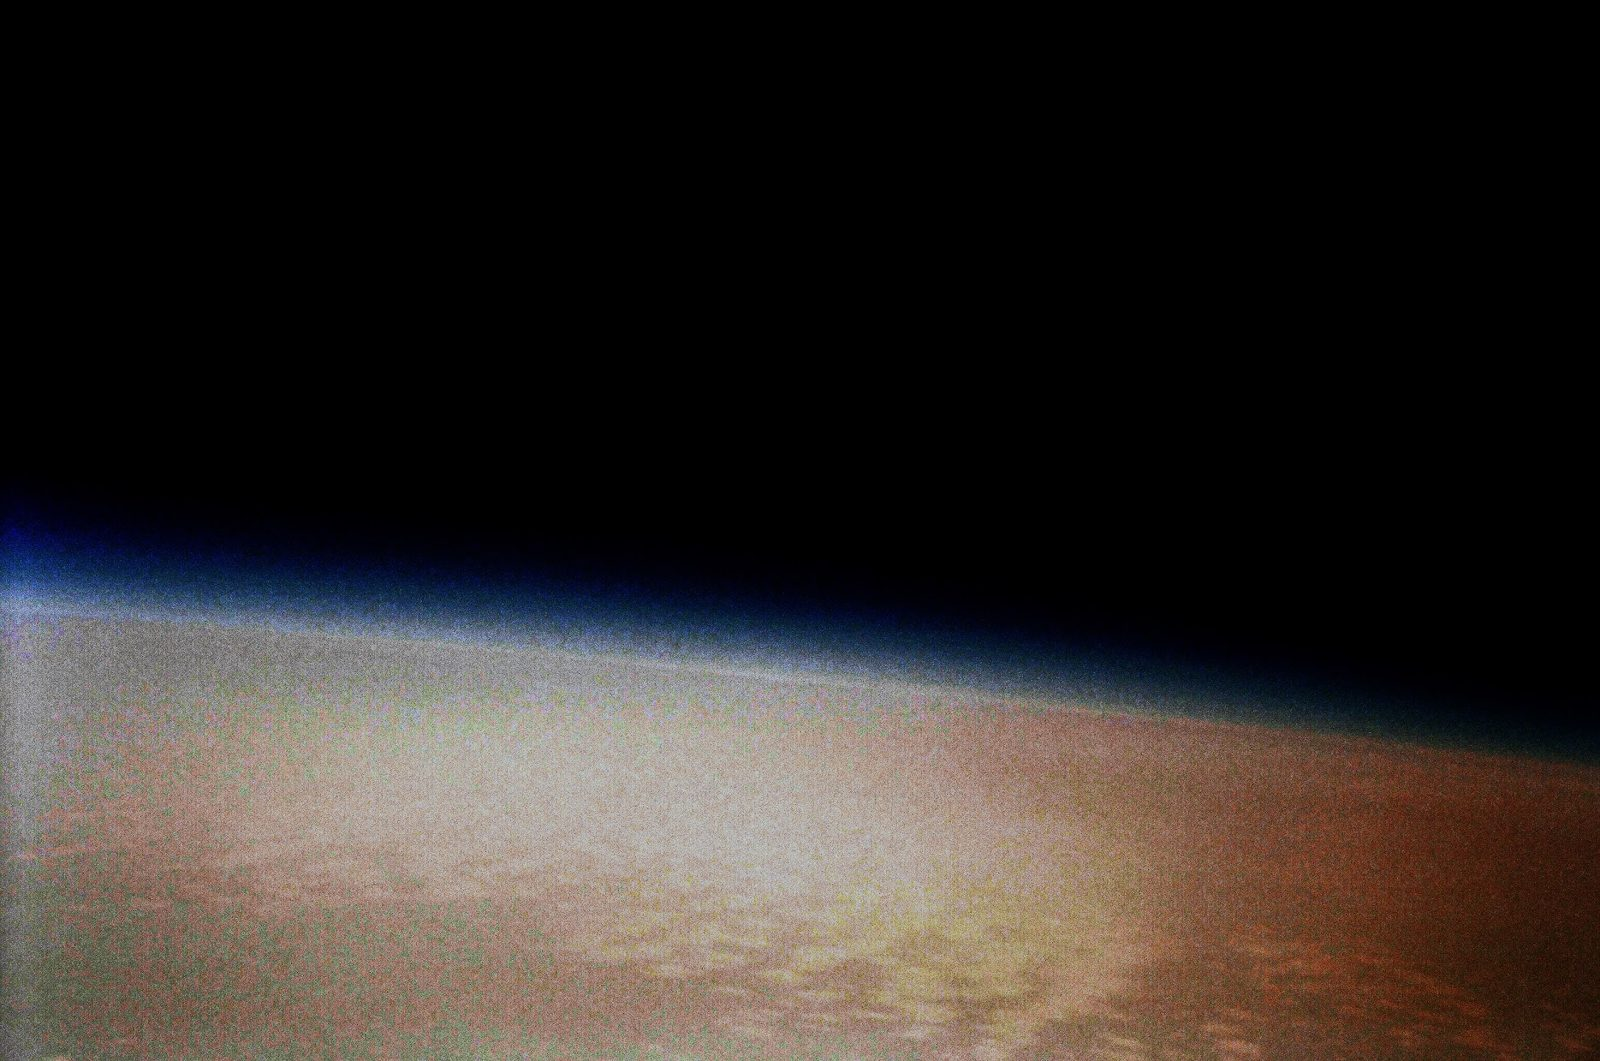
\includegraphics[width=\paperwidth]{2023_zdjecie_analogowe_stratosfera}};
    \end{scope}
    \node[anchor=south east,font=\sffamily\scriptsize,text=white] at ([xshift=-5mm,yshift=-210mm]current page.north east)
      {Zdjęcie z aparatu analogowego na pokładzie, misja z 26.05.2023};
    \node[anchor=north east,inner sep=0] at ([xshift=-15mm,yshift=-12mm]current page.north east)
      {\href{https://www.simle.pl}{
\includegraphics[width=38mm,trim=69.6 67.2 69.1 67.2,clip]{SimLE_logo_achromatyczny_bialy}}};
  \end{tikzpicture}
  \vspace*{12mm}
  {\color{white}
   {\large\color{sdorange}KOŁO NAUKOWE SIMLE \textbullet{} POLITECHNIKA GDAŃSKA\par}
   \vspace{10mm}
   {\fontsize{40}{44}\selectfont\bfseries Stardust NEXT\par}
   \vspace{4mm}
   {\Huge Manual misji stratosferycznych\par}
   \vspace{6mm}
   {\Large Od celu misji do raportu po locie\par}}
  \vfill
  \begin{minipage}[b]{0.5\linewidth}
    \large\color{sdnavy}
    Dokumentacja platformy balonowej\\z odcinaczem mechanicznym\par
    \vspace{6mm}\normalsize\color{sdgray}
    Wersja dokumentu: \wersja\\
    Data: \datawersji\\[3mm]
    Koło Naukowe SimLE: \href{https://www.simle.pl}{\color{sdnavy}www.simle.pl}
  \end{minipage}\hfill
  \begin{minipage}[b]{0.22\linewidth}\centering
    \href{https://www.simle.pl}{
\includegraphics[width=\linewidth]{SimLE_znak_podstawowy_kadr}}
  \end{minipage}\hspace{6mm}
  \begin{minipage}[b]{0.18\linewidth}\raggedleft
    
\includegraphics[width=\linewidth]{SimLE_Stardust_2023}
  \end{minipage}
  \restoregeometry
\end{titlepage}

% ---------------------------------------------------------------- metryczka
\cleardoublepage
\thispagestyle{empty}
\vspace*{\fill}
\begin{blok}
{\sffamily\large\color{sdnavy}\textbf{Pierwsze wydanie:} Marcin Jasiukowicz, 2026}\par\smallskip
{\itshape Bardzo opóźnione -- misje z 2023 roku czekały na swój manual trzy lata.\\
Ku chwale kolejnym pokoleniom baloniarzy!\par}
\bigskip
{\sffamily\bfseries\large\color{sdnavy} O tym dokumencie\par}\medskip
Ten dokument daje niezbędne minimum, aby nowy zespół wyjął sprzęt z szafki i wykonał misję balonu stratosferycznego na platformie Stardust NEXT.

Dokument jest przygotowany do druku dwustronnego i bindowania. Wydrukuj go w całości. Formularze z dodatku~\ref{dod:formularze} wydrukuj osobno dla każdej misji i wypełniaj długopisem. Notatki z terenu zapisuj na stronach „Notatki terenowe” na końcu dokumentu.

\medskip
\renewcommand{\arraystretch}{1.5}
\begin{tabularx}{\linewidth}{@{}lL@{}}
\toprule
Wydanie & pierwsze (2026), opracowanie: Marcin Jasiukowicz \\
Wersja dokumentu & \wersja \\
Data wydania & \datawersji \\
Koło Naukowe SimLE & \www{www.simle.pl} \\
Źródło & \www{github.com/simle-stardust/Manual} \\
Kontakt & \href{mailto:stardust@simle.pl}{\nolinkurl{stardust@simle.pl}} \\
Licencja & Dokumentacja koła naukowego SimLE, Politechnika Gdańska \\
\bottomrule
\end{tabularx}

\medskip
\textbf{Dokument publiczny.} Ten dokument jest publiczny. Nie wpisuj do niego danych osobowych ani treści z wewnętrznej dokumentacji koła. Wypełnione formularze przechowuj wewnątrz zespołu.

\textbf{Zgłaszanie poprawek.} Gdy znajdziesz błąd albo procedura się zmieni, zapisz to w notatkach terenowych i przenieś do repozytorium dokumentacji po misji (\rozdz{ch:projekt}).
\end{blok}
\vspace*{\fill}

\cleardoublepage
\pagenumbering{roman}
\tableofcontents
\cleardoublepage
\pagenumbering{arabic}

\chapter{Wprowadzenie}\label{ch:wprowadzenie}

\begin{sekcja}{Cel dokumentu}
Ten dokument opisuje, jak przygotować i wykonać misję balonu stratosferycznego na platformie Stardust NEXT. Platforma to mały balon lateksowy z gondolą z pudełek styropianowych i odcinaczem mechanicznym.

Dokument daje niezbędne minimum, aby nowy zespół wyjął sprzęt z szafki i wykonał misję. Dokument jest ogólny: działa dla każdej przyszłej misji. Dane konkretnych misji są tylko w rozdziale~\ref{ch:historia} i w wypełnionych formularzach.

Dokument zawiera:
\begin{itemize}
  \item historię platformy i wnioski z poprzednich lotów,
  \item planowanie misji: od celu i ładunku do decyzji o starcie,
  \item wymagania prawne,
  \item segment naziemny: stanowisko startowe, tankowanie, stacje odbiorcze,
  \item segment lotny: powłoka, spadochron, olinowanie, odcinacz, gondola,
  \item elektronikę i łączność radiową,
  \item oprogramowanie do predykcji i śledzenia,
  \item instrukcje montażu i wykaz materiałów,
  \item zasady prowadzenia projektu i dokumentacji,
  \item formularze do druku i notatki terenowe.
\end{itemize}
\end{sekcja}

\begin{sekcja}{Jak używać tego dokumentu}
\begin{enumerate}
  \item Przeczytaj rozdział~\ref{ch:historia} „\nameref{ch:historia}”. Wnioski z poprzednich lotów wyjaśniają, dlaczego procedury wyglądają tak, jak wyglądają.
  \item Zacznij planowanie od rozdziału~\ref{ch:planowanie} „\nameref{ch:planowanie}”, co najmniej 3--4 miesiące przed planowanym lotem.
  \item Sprawdź sprzęt z szafki według rozdziału~\ref{ch:materialy} „\nameref{ch:materialy}”.
  \item Wydrukuj formularze z dodatku~\ref{dod:formularze}. Wypełniaj je długopisem w trakcie przygotowań i w dniu startu.
  \item Po misji przenieś notatki terenowe i wnioski do repozytorium dokumentacji.
\end{enumerate}

W tekście są dwa rodzaje ramek:

\begin{uwaga}Informacja o zagrożeniu dla ludzi, sprzętu albo powodzenia misji.\end{uwaga}

\begin{wskazowka}Praktyczna rada z poprzednich misji.\end{wskazowka}
\end{sekcja}

\begin{sekcja}{Najpierw bezpieczeństwo i rozsądek}
Ten dokument jest wzorem, nie przepisem. Procedury i dokumentacja są ważne, ale najważniejsze jest to, aby misja przebiegła bezpiecznie i aby wszyscy dobrze się bawili.

\begin{itemize}
  \item Nie stresuj się, że pominiesz jakiś krok, jeżeli możesz się upewnić, że mimo to wszystko będzie bezpieczne. Rozsądek przede wszystkim.
  \item Dopasuj procedury do swojej misji. Gdy coś nie pasuje -- zmień to i zapisz dlaczego.
  \item Balon stratosferyczny to jeden z najprostszych sposobów, aby zdobyć praktyczne doświadczenie w całym przekroju projektu: od celu naukowego, przez budowę i testy, formalności i logistykę, do analizy wyników.
  \item Publikuj wyniki na konferencjach -- w szczególności na sympozjum ESA PAC (\emph{ESA Symposium on European Rocket and Balloon Programmes and Related Research}). Inne miejsca dla studenckich projektów balonowych: konferencja AHAC i czasopismo \emph{Journal of High Altitude Ballooning}~\cite{sba}. Czytaj artykuły naukowe z tych i innych konferencji.
\end{itemize}

\begin{center}\sffamily\large\color{sdorange} Stay curious, have fun.\end{center}
\end{sekcja}

\begin{sekcja}{Platforma Stardust NEXT}
Platforma Stardust NEXT to zestaw sprzętu i procedur do lotów balonów stratosferycznych. Koło Naukowe SimLE (Politechnika Gdańska) opracowało platformę na podstawie doświadczeń z projektu Stardust~\cite{iac2023,pac2024}.

Platforma ma trzy zadania:
\begin{enumerate}
  \item Wynieść ładunek badawczy do stratosfery i bezpiecznie sprowadzić go na ziemię.
  \item Oddzielić elektronikę platformy od ładunku. Zespół platformy i zespół badawczy pracują niezależnie. Ładunek musi tylko zmieścić się w standardowym pudełku i w limicie masy.
  \item Używać powtarzalnych komponentów i procedur, aby każdy nowy skład zespołu mógł wykonać misję.
\end{enumerate}

\dwafoto{2023_zestaw_przed_startem}{Zestaw lotny przed startem: gondola gotowa, olinowanie rozłożone, w tle tankowanie powłoki (26.05.2023).}
{2023_balon_po_tankowaniu}{Powłoka po tankowaniu, przytrzymywana folią przed startem (26.05.2023).}
\end{sekcja}

\begin{sekcja}{Typowy lot}
Typowy lot balonu lateksowego trwa około 2,5--3 godzin (rysunek~\ref{fig:profil-typowy}):
\begin{enumerate}
  \item Wznoszenie z prędkością około \SI{5}{m/s}.
  \item Pęknięcie powłoki na wysokości około 28--35~km albo odcięcie ładunku przez odcinacz.
  \item Opadanie na spadochronie. Wysoko spadochron opada bardzo szybko, bo powietrze jest rzadkie. Przy ziemi prędkość spada do około \SI{5}{m/s}.
  \item Lądowanie w odległości od kilkunastu do ponad 100~km od miejsca startu. Odległość zależy od wiatru.
\end{enumerate}

\begin{center}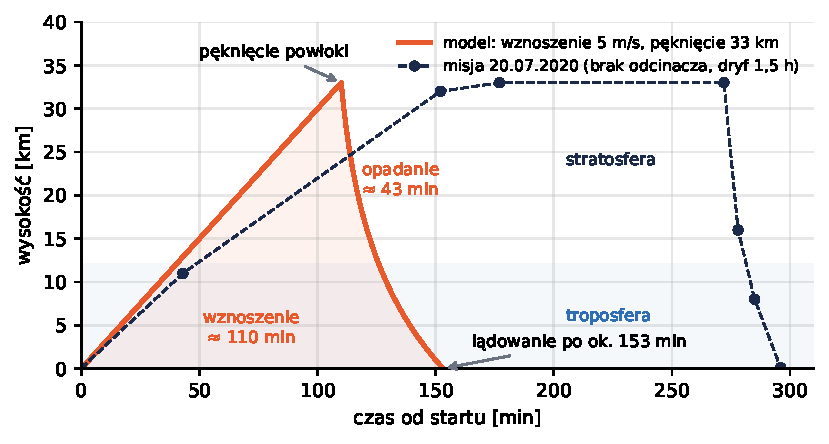
\includegraphics[width=\linewidth]{profil_typowy}\end{center}
\captionof{figure}{Typowy lot: model (wznoszenie \SI{5}{m/s}, pęknięcie na \SI{33}{km}) i dane misji z 20.07.2020. W 2020 roku balon nie pękł na przewidywanej wysokości i dryfował prawie 2~h na \SI{33}{km}, bo nie miał odcinacza~\cite{raport2020}.}\label{fig:profil-typowy}
\end{sekcja}

\begin{sekcja}{Warunki w stratosferze}
Stratosfera to warstwa atmosfery od około 12--15 do \SI{50}{km}. Warunki w stratosferze:
\begin{itemize}
  \item temperatura powietrza do około \SI{-60}{\degreeCelsius},
  \item ciśnienie poniżej \SI{100}{hPa}; na wysokości \SI{33}{km} około \SI{7}{hPa} -- to prawie próżnia,
  \item silne promieniowanie UV i kosmiczne,
  \item bardzo słaba wymiana ciepła z powietrzem: elektronika nie oddaje ciepła przez konwekcję i może się przegrzać mimo mrozu (rozdział~\ref{ch:elektronika}).
\end{itemize}
\foto[0.85\linewidth]{2020_kamera_pokladowa_stratosfera}{Widok z kamery pokładowej 360° w troposferze (20.07.2020). Zakrzywienie horyzontu to efekt obiektywu typu rybie oko. Bateria kamery wyczerpała się po około 30 minutach lotu~\cite{raport2020}.}
\end{sekcja}

\begin{sekcja}{Architektura misji}
Misja ma dwa segmenty.

\begin{minipage}[t]{0.47\linewidth}
\textbf{Segment naziemny} (rozdział~\ref{ch:naziemny}):
\begin{itemize}
  \item stanowisko startowe,
  \item zestaw do tankowania,
  \item stacja odbiorcza stacjonarna,
  \item stacja odbiorcza mobilna w samochodzie pościgowym,
  \item oprogramowanie do planowania, predykcji i śledzenia.
\end{itemize}
\end{minipage}\hfill
\begin{minipage}[t]{0.47\linewidth}
\textbf{Segment lotny} (rozdział~\ref{ch:lotny}), od góry:
\begin{enumerate}
  \item powłoka z helem,
  \item krętlik,
  \item spadochron,
  \item olinowanie z odcinaczem,
  \item gondola platformy,
  \item gondola ładunku.
\end{enumerate}
\end{minipage}
\end{sekcja}

\begin{sekcja}{Fazy misji}
Misja to zwieńczenie kilku miesięcy przygotowań. Sam lot trwa kilka godzin. Nazwy faz odpowiadają typowym fazom projektu (inicjacja, planowanie, realizacja, zamknięcie) i kampanii startowej programów takich jak BEXUS.

\renewcommand{\arraystretch}{1.35}
\begin{tabularx}{\linewidth}{@{}P{30mm}LP{36mm}@{}}
\toprule
\textbf{Faza} & \textbf{Zadania} & \textbf{Rozdział / formularz}\\\midrule
Inicjacja & Cel misji, wymagania ładunku, projekt i budowa eksperymentu. & \ref{ch:planowanie}, F2\\
Planowanie lotu & Bilans masy, ilość gazu, predykcja trajektorii, wybór terminów i miejsc. & \ref{ch:planowanie}, F4\\
Formalności & Klasa balonu, zgłoszenie do PAŻP, ubezpieczenie, licencja radiowa. & \ref{ch:prawo}, F3\\
Budowa i testy & Montaż, testy w zimnie, zasięgu, odcinacza, czasu pracy. & \ref{ch:montaz}, F5\\
Przegląd gotowości & Przegląd gotowości do startu: decyzja „leci / nie leci”. & \ref{ch:planowanie}, F6\\
Start & Kampania startowa: stanowisko, tankowanie, start. & \ref{ch:naziemny}, F9--F11\\
Lot i pościg & Odbiór telemetrii, jazda w kierunku predykcji. & \ref{ch:oprogramowanie}, F12\\
Odzyskanie & Lokalizacja ładunku, zabezpieczenie danych. & F13\\
Analiza i zamknięcie & Raport, wnioski, aktualizacja dokumentacji. & \ref{ch:projekt}, F14\\
\bottomrule
\end{tabularx}
\end{sekcja}

\chapter{Historia i wnioski}\label{ch:historia}

\begin{sekcja}{Skąd pochodzi platforma}
Zespół Stardust (Koło Naukowe SimLE, Politechnika Gdańska) wypuszcza balony stratosferyczne od 2016 roku. Pierwszą próbę startu zespół podjął w 2015 roku -- balon nie wzniósł się w powietrze (sekcja~\ref{sec:proba2015}). Pierwsze misje własne (2016--2020) służyły badaniom mikroorganizmów w stratosferze. W 2021 roku eksperyment Stardust poleciał na balonie BEXUS~30 w programie REXUS/BEXUS~\cite{iac2023,praca2022}. Po tym programie starsi członkowie skończyli studia. Nowy zespół, Stardust NEXT, zbudował małą platformę, którą może powtórzyć każdy nowy skład zespołu~\cite{pac2024}.

Praktyki projektowe z programu REXUS/BEXUS opisuje rozdział~\ref{ch:projekt}.

Po każdej misji dopisz wiersz do tabeli~\ref{tab:misje} i nowe wnioski do tabeli~\ref{tab:wnioski}.
\end{sekcja}

\begin{sekcja}{Misje własne}
\renewcommand{\arraystretch}{1.3}
\small
\begin{tabularx}{\linewidth}{@{}P{16mm}P{12mm}LP{12mm}P{36mm}P{15mm}@{}}
\toprule
\textbf{Data} & \textbf{Start} & \textbf{Ładunek} & \textbf{Pułap} & \textbf{Wynik} & \textbf{Źródła}\\\midrule
2015 & Polska & Pierwsza próba startu & -- & Start przerwany, balon nie poleciał. & relacja zespołu\\
26.04.2016 & Polska & Gondola ze styroduru, dwa moduły Arduino, odcinacz z drutem oporowym & -- & Pierwszy lot. Lądowanie na drzewie -- gondolę zdjęła straż pożarna podnośnikiem. & \cite{iac2023,stardustweb,dok2018}\\
27.09.2017 & Toruń & Układ próbkujący (test sterylności), odcinacz z drutem oporowym (zegar) & ok. 30 km & Balon pękł przed czasem odcięcia. Lądowanie przy małym cieku (Kotomierz). & \cite{magrian2018,iac2023,stardustweb}\\
05.2018 & Toruń & Układ próbkujący (2 filtry), grzałki, licznik Geigera, ładunek gościnny & 24,8 km & Sukces. & \cite{iac2023}\\
20.07.2020 & Toruń & Test układu dla BEXUS, ok. 4 kg, 2 gondole & 33,3 km & Brak odcinacza. Dryf 1,5 h. Lądowanie ok. 90 km od startu. & \cite{raport2020,praca2022}\\
27.02.2022 & Iława & Radiosonda z kamerą (lot szkoleniowy) & 33,4 km & Sukces. Lądowanie 51 km od startu, okolice Brodnicy. & \cite{blog2022,pac2024}\\
26.05.2023 & Iława & Platforma NEXT: OBC, łączność, odcinacz serwomechaniczny & 34 km & Odcinacz nie zadziałał. Lądowanie 23 km od startu. & \cite{blog2023,go2023,infoilawa2023,pac2024}\\
09.08.2023 & Polska & Platforma NEXT + ładunek STORM & -- & Odcinacz z drutem oporowym nie zadziałał. Ładunek zebrał dane. & \cite{pac2024,storm}\\
\midrule
\multicolumn{6}{@{}l}{\footnotesize\itshape Kolejne misje dopisuj poniżej:}\\[3mm]
\rule{0pt}{6mm} & & & & & \\\hline
\rule{0pt}{6mm} & & & & & \\\hline
\end{tabularx}
\captionof{table}{Misje balonowe zespołu Stardust. Źródła (artykuły, wpisy, media) -- w spisie literatury.}\label{tab:misje}
\end{sekcja}

\begin{sekcja}{Pierwsza próba (2015)}\label{sec:proba2015}
Pierwsza misja zespołu miała się odbyć w 2015 roku. Start był szeroko zapowiadany w mediach: było odliczanie, a nawet transmisja na żywo. Balon nie wzniósł się w powietrze i start się nie odbył.

Z tej próby zostały dwie lekcje:
\begin{enumerate}
  \item \textbf{Pierwsze próby zaczynają się od porażek.} Porażka jest częścią nauki i doskonalenia. Zapisz, co się stało, i popraw to w następnej misji.
  \item \textbf{Bezpieczeństwo przede wszystkim.} Przerwij start, gdy coś jest nie tak -- niezależnie od presji z zewnątrz: mediów, gości, sponsorów, transmisji na żywo.
\end{enumerate}
\begin{uwaga}Kierownik startu i kierownik misji mają prawo i obowiązek powiedzieć „no-go”. Zapowiedź w mediach nie jest powodem do startu.\end{uwaga}
\end{sekcja}

\begin{sekcja}{Pierwszy lot (26.04.2016)}
\noindent\begin{minipage}[t]{0.6\linewidth}\vspace{0pt}
Dokumentacja projektu~\cite{dok2018} opisuje platformę z pierwszych lotów (rysunki oznaczone rokiem 2016):
\begin{itemize}
  \item gondola ze styroduru (około $29\times29\times\SI{28}{cm}$), laminowana tkaniną szklaną \SI{48}{g/m^2} i żywicą epoksydową,
  \item balon lateksowy \SI{1200}{g}, około \SI{6}{m^3} helu; tankowanie trwało około 1,5 godziny,
  \item moduł A (Arduino Nano): czujniki ciśnienia, temperatury i wilgotności, GPS, zegar, karta SD,
  \item moduł B: próba stabilizacji obrotu gondoli kołem reakcyjnym oraz Bluetooth do sprawdzenia elektroniki tuż przed startem,
  \item odcinacz z drutem oporowym w obudowie drukowanej z ABS, krętlik nad odcinaczem.
\end{itemize}
Gondola wylądowała na drzewie. Zdjęła ją straż pożarna podnośnikiem (rysunek~\ref{fig:2016drzewo}).

Już wtedy zespół zauważył, że APRS bywa nieodbierany poniżej około \SI{200}{m}, i do poszukiwań używał trackera oraz ręcznego odbiornika APRS.
\end{minipage}\hfill
\begin{minipage}[t]{0.36\linewidth}\vspace{0pt}\centering
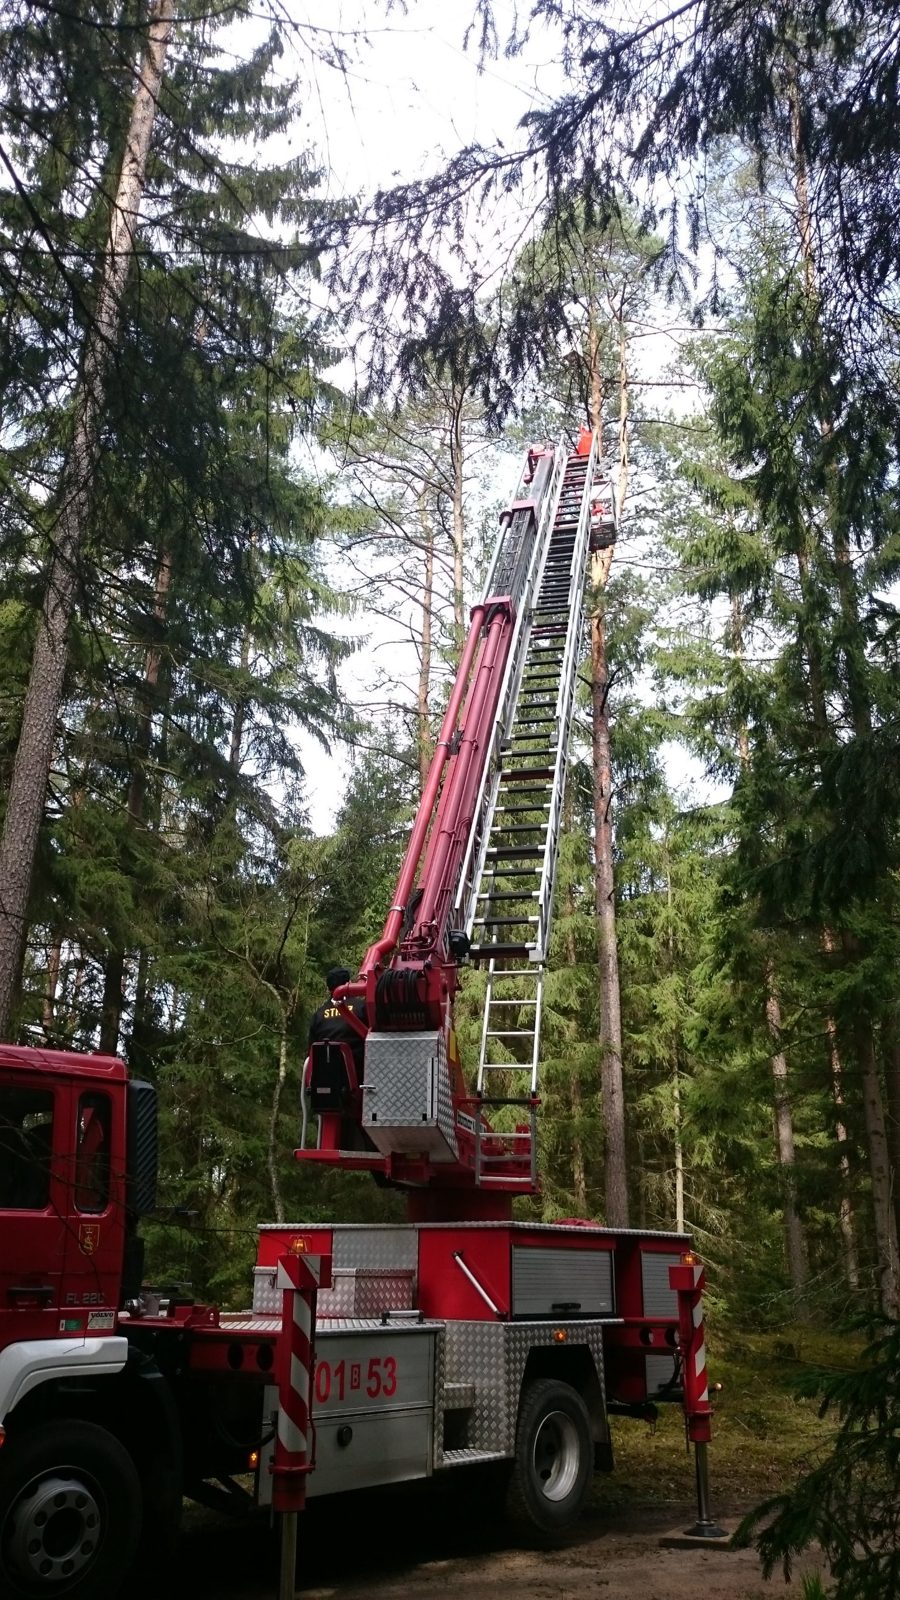
\includegraphics[width=\linewidth]{2016_gondola_drzewo_podnosnik}
\captionof{figure}{Gondola na drzewie po pierwszym locie (2016). Straż pożarna zdjęła ją podnośnikiem.}\label{fig:2016drzewo}
\end{minipage}
\end{sekcja}

\begin{sekcja}{Pierwsza misja mikrobiologiczna (27.09.2017)}
Lot testowy układu pobierającego próbki mikrobiologiczne, opisany w pracy inżynierskiej Szymona Magriana i Karola Pelznera~\cite{magrian2018}. Cel: sprawdzić sterylność układu i wszystkie podzespoły w stratosferze. Gondola ze styroduru z wkładką z plexi, masa \SI{2.6}{kg}, balon Hwoyee \SI{1600}{g}, hel, spadochron okrągły \SI{1}{m}. Start z Torunia o 10:06~UTC, lądowanie o 12:08~UTC.

Co się wydarzyło i czego to uczy:
\begin{itemize}
  \item \textbf{Odcinacz z drutem oporowym działał według zegara.} Czas odcięcia (11:30~UTC) wynikał z predykcji. Balon wznosił się szybciej i pękł wcześniej (11:24~UTC). Drut się rozgrzał, ale bez naciągu linki nie przepalił jej. Wniosek: drut oporowy przecina linkę tylko pod obciążeniem, a odcinacz powinien działać według wysokości, nie tylko zegara.
  \item \textbf{Usterki elektroniki:} karta SD wypadła z gniazda od wstrząsów (zapis tylko z pierwszych 30 minut), przewód czujnika ciśnienia urwał się przy starcie, część czujników nie zapisała danych. Przyczyna: płytka prototypowa i słabe mocowania. Wniosek: płytka PCB, pewne mocowania, test wstrząsów i diody stanu do kontroli przed startem.
  \item \textbf{Kamery} przesunęły się w czasie przygotowań -- część obrazu zasłonił styrodur. Wniosek: sprawdź kadr tuż przed zamknięciem gondoli.
  \item \textbf{Odzyskanie:} ostatnia pozycja APRS pochodziła z wysokości \SI{167}{m}. Gondolę znalazł zespół dzięki telefonowi w gondoli i brzęczykowi (wysoka trawa). Gondola wylądowała około \SI{3}{m} od małego kanału -- gondola musi pływać.
  \item \textbf{Spadochron:} średnia prędkość opadania poniżej \SI{2.8}{km} wyniosła \SI{5.45}{m/s} dla \SI{2.6}{kg} i spadochronu \SI{1}{m}.
\end{itemize}
\end{sekcja}

\begin{sekcja}{Misja mikrobiologiczna (2018)}
Ładunek z grzaną sekcją na komórki, pompą i licznikiem Geigera. Dane z rejestratora pokładowego i z APRS pokazuje rysunek~\ref{fig:misja2018}.

\begin{center}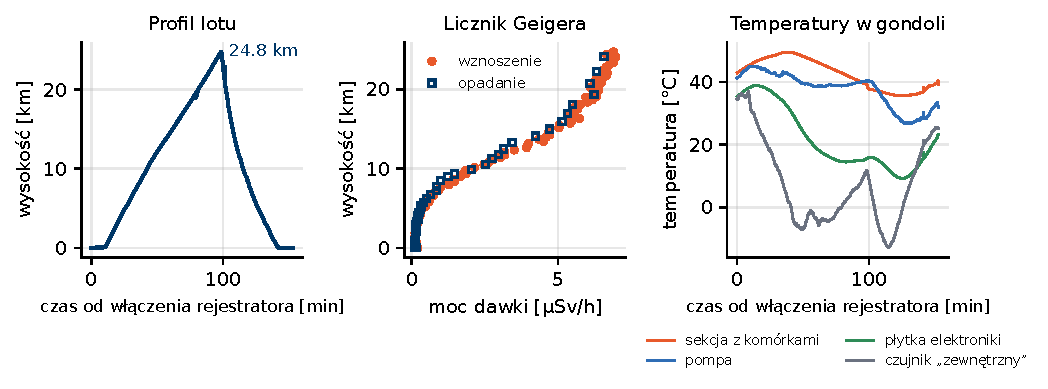
\includegraphics[width=\linewidth]{misja_2018}\end{center}
\captionof{figure}{Misja mikrobiologiczna z 2018 roku (okolice Torunia): profil lotu, moc dawki z licznika Geigera i temperatury w gondoli. Dane: \texttt{data/2018\_mikrobiologia\_*.csv}.}\label{fig:misja2018}

\begin{itemize}
  \item Pułap \SI{24.8}{km}. Moc dawki rosła z wysokością: od około \SI{0.13}{\micro Sv/h} przy ziemi do około \SI{7}{\micro Sv/h} na \SI{23}{}--\SI{25}{km}.
  \item Grzałki utrzymały sekcję z komórkami w zakresie 36--\SI{50}{\degreeCelsius}. Płytka elektroniki ochłodziła się do około \SI{9}{\degreeCelsius}.
  \item Czujnik opisany jako „zewnętrzny” pokazał minimum \SI{-13}{\degreeCelsius}, a powietrze na wysokości 10--\SI{12}{km} ma około \SI{-50}{\degreeCelsius}. Czujnik mierzył ściankę gondoli, nie powietrze. Wniosek: czujnik temperatury powietrza musi wystawać z gondoli i mieć osłonę przed słońcem.
  \item Czujnik ciśnienia nie podawał wartości powyżej około \SI{18}{km} (\SI{52}{hPa}). Sprawdź zakres czujnika w karcie katalogowej.
\end{itemize}
\end{sekcja}

\begin{sekcja}{Trasy lotów}
Rysunek~\ref{fig:mapa} pokazuje trasy lotów z dostępnymi danymi. Przy wietrze z zachodu balon leci na wschód -- w stronę granicy z Rosją (obwód królewiecki) i Białorusią. Predykcja trajektorii jest więc warunkiem każdego startu (rozdział~\ref{ch:planowanie}).

\begin{center}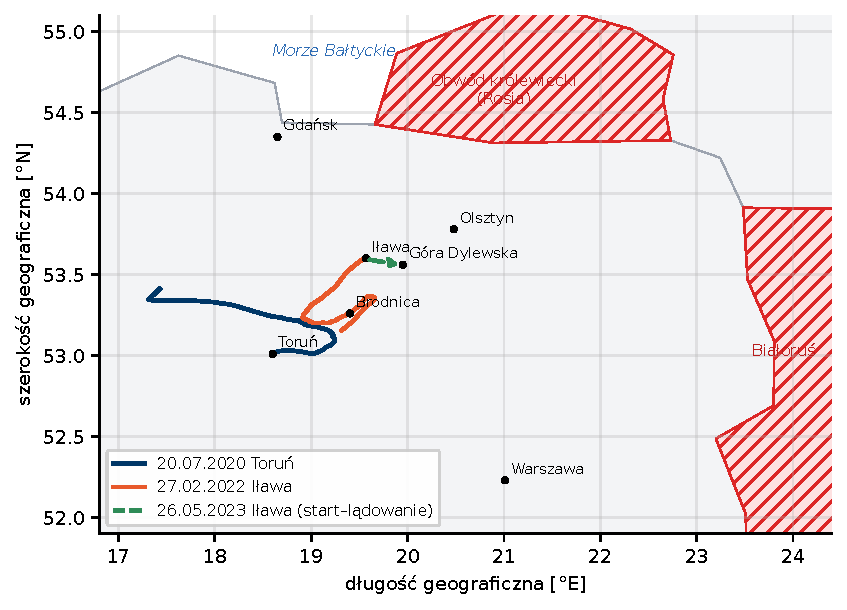
\includegraphics[width=0.92\linewidth]{mapa_lotow}\end{center}
\captionof{figure}{Trasy lotów z lat 2020--2023. Kreskowane obszary: państwa, nad którymi lot i lądowanie są niedopuszczalne.}\label{fig:mapa}
\end{sekcja}

\begin{sekcja}{Profil lotu w przestrzeni}
\begin{center}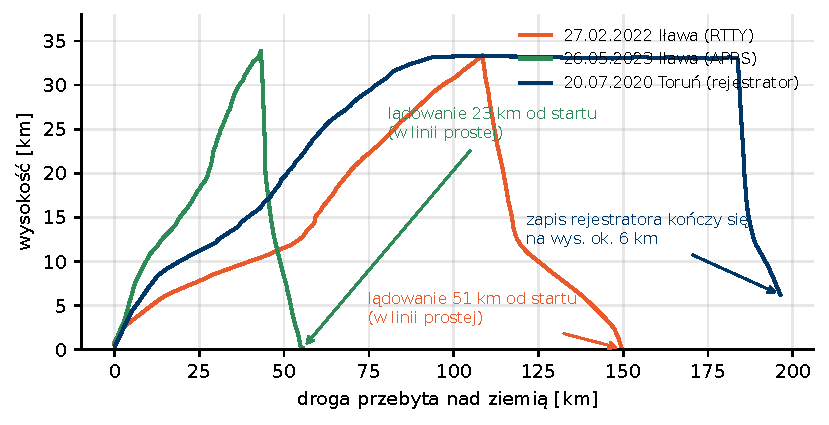
\includegraphics[width=\linewidth]{profil_dystans}\end{center}
\captionof{figure}{Wysokość w funkcji drogi przebytej nad ziemią. Dane z trackera (2022) i z rejestratora pokładowego (2020).}\label{fig:profil-dystans}

\foto[\linewidth]{2022_profil_lotu_2022_google_earth}{Profil misji z 27.02.2022 w Google Earth. Po prawej Zatoka Gdańska.}
\end{sekcja}

\begin{sekcja}{Lot szkoleniowy (27.02.2022)}
Cel: nauczyć nowy zespół procedur. Ładunek: radiosonda z kamerą, telemetria RTTY i APRS pod znakiem SR0FLY (SR0FLY-12), użytym za zgodą jego właściciela (rozdział~\ref{ch:prawo}).

Zespół ćwiczył trzy fazy:
\begin{enumerate}
  \item przygotowanie sprzętu i stanowiska startowego,
  \item tankowanie i start,
  \item śledzenie, pościg samochodem, odzyskanie.
\end{enumerate}

\begin{wskazowka}Ten format to wzór dla każdej nowej grupy: pierwsza misja ma prosty ładunek i skupia się na procedurach.\end{wskazowka}

\dwafoto{2022_stanowisko_zabezpieczone}{Stanowisko startowe: plandeka i folia dociśnięte skrzynkami (27.02.2022).}
{2022_poscig_samochod}{Pościg: laptop z mapą śledzenia i radiotelefon w samochodzie (27.02.2022).}
\end{sekcja}

\begin{sekcja}{Test platformy (26.05.2023)}
Pierwsza misja, którą nowy zespół zaprojektował i zbudował samodzielnie. Testowane systemy: komputer pokładowy (OBC), łączność i namierzanie, olinowanie z odcinaczem mechanicznym, gondola z pudełek styropianowych. Lot: \SI{34}{km} po około 90 minutach, lądowanie w okolicy Góry Dylewskiej~\cite{blog2023}.

Odcinacz był w gondoli, nie pod balonem. Powód: zespół nie miał doświadczenia z odcinaczem sterowanym zdalnie pod powłoką. Serwo w gondoli miało zwolnić linkę, która trzyma balon.

\textbf{Problem:} odcinacz nie zadziałał. Gondola obracała się w locie. Krętlik był tylko na górze olinowania. Na dole linki skręciły się i linka odcinacza nie mogła się zwolnić~\cite{pac2024}.

\textbf{Zabezpieczenie, które zadziałało:} zapas 10--15~m linki odcinacza między krętlikiem a spadochronem. Spadochron miał miejsce na rozwinięcie mimo skręconych linek. Zestaw wylądował bezpiecznie.

\foto[0.7\linewidth]{2020_odzysk_resztki_powloki}{Po lądowaniu: resztki pękniętej powłoki i gondola (20.07.2020).}
\end{sekcja}

\begin{sekcja}{Ładunek STORM (09.08.2023)}
Pierwsza misja nowego zespołu bez pomocy starszych członków. Zespół zmniejszył masę komponentów i zastąpił odcinacz serwomechaniczny odcinaczem z drutem oporowym. Olinowanie bez zmian.

\textbf{Problem:} drut oporowy grzał się za krótko i nie przeciął linki~\cite{pac2024}.
\end{sekcja}

\clearpage
\section{Wnioski}
Stosuj te wnioski w każdej misji.

\renewcommand{\arraystretch}{1.3}
\begin{longtable}{@{}P{27mm}>{\raggedright\arraybackslash}p{0.62\linewidth}P{12mm}@{}}
\toprule
\textbf{Obszar} & \textbf{Wniosek} & \textbf{Misja}\\\midrule\endhead
\bottomrule\endfoot
Odcinacz & Każdy lot musi mieć odcinacz. Bez odcinacza balon może dryfować godzinami i wylądować daleko. & 2020\\
Odcinacz & Testuj odcinacz w warunkach lotu: zimno, obrót gondoli, skręcone linki, pełne obciążenie. Daj drugi, niezależny odcinacz innego typu. & 2023\\
Odcinacz & Drut oporowy musi dostać prąd wystarczający do przecięcia linki. Sprawdź to z docelowym tranzystorem i baterią, wiele razy i w zimnie. & 2023\\
Olinowanie & Gondola obraca się w locie. Daj krętlik pod balonem i zapas linki odcinacza nad spadochronem. Poprzeczki na linkach mogą ograniczyć skręcanie (do sprawdzenia kamerą w locie). Długość zapasu to wciąż eksperyment: próbuj krótszej i zapisz wynik. & 2023\\
Gaz & Butla może mieć mniej gazu, niż deklaruje dostawca. Zamów gaz z zapasem. Mierz siłę nośną obciążnikiem. & 2020\\
Wysokość & Wzór na wysokość z ciśnienia działa tylko do około 10~km. Powyżej używaj GPS. & 2020\\
Czujniki & Czujnik BME280 nie mierzy poniżej \SI{300}{hPa}. Odrzucaj kody błędów czujników w programie. & 2020\\
Anteny & Źle zmontowana antena wyłączyła APRS. Sprawdzaj odbiór z odległości co najmniej \SI{100}{m}. & 2020\\
Śledzenie & Używaj co najmniej dwóch niezależnych systemów śledzenia i lokalizatorów po lądowaniu. & 2020\\
Łączność wewn. & Nie używaj WiFi między gondolami. Używaj kabla albo osobnego GPS w każdej gondoli. & 2020\\
Zasilanie & Każde urządzenie (także kamera) musi działać przez cały lot z zapasem. Kamera bez zewnętrznej baterii wyłączyła się po 30 minutach. & 2020\\
Termika & Elektronika w izolowanej gondoli może się przegrzać latem (ponad \SI{50}{\degreeCelsius}). & 2020\\
Mechanika & Mocuj elektronikę na wkładce. Dystanse PCB pękły przy lądowaniu. & 2020\\
Montaż & Każdy podzespół ma osobę odpowiedzialną albo opisaną procedurę montażu. & 2020\\
Diagnostyka & Dodaj diody statusu, aby szybko sprawdzić stan systemu na stanowisku. & 2020\\
Planowanie & Wiatr decyduje o trasie lotu. Planuj start z predykcją trajektorii. & 2016\\
Bezpieczeństwo & Przerwij start, gdy coś jest nie tak -- niezależnie od presji mediów, gości i sponsorów. Porażka jest częścią nauki. & 2015\\
Odcinacz & Drut oporowy przecina linkę tylko pod obciążeniem: po pęknięciu balonu nie przetnie. Odcinaj według wysokości, nie tylko zegara. & 2017\\
Mechanika & Karta SD wypadła z gniazda od wstrząsów, przewody urwały się przy starcie. Używaj PCB i pewnych mocowań, testuj wstrząsy. & 2017\\
Kamery & Kamera przesunęła się w czasie przygotowań. Sprawdź kadr tuż przed zamknięciem gondoli. & 2017\\
Odzyskanie & Gondola może zawisnąć na drzewie. Przygotuj kontakt do arborysty albo firmy z podnośnikiem. & 2016\\
Odzyskanie & Ostatnia pozycja APRS bywa z wysokości kilkuset metrów. Telefon albo lokalizator w gondoli i brzęczyk pozwalają znaleźć gondolę. & 2017\\
Gondola & Gondola musi pływać i być szczelna. Sprawdź ją w wannie z wodą, z obciążeniem do docelowej masy. & 2017\\
Czujniki & Czujnik temperatury powietrza musi wystawać z gondoli i mieć osłonę przed słońcem. Sprawdź zakres czujnika ciśnienia. & 2018\\
Zespół & Pierwsza misja nowego zespołu to lot szkoleniowy z prostym ładunkiem. & 2022\\
% Puste wiersze dopełniają stronę na nowe wnioski.
\rule{0pt}{7mm} & & \\\hline
\rule{0pt}{7mm} & & \\\hline
\rule{0pt}{7mm} & & \\\hline
\rule{0pt}{7mm} & & \\\hline
\rule{0pt}{7mm} & & \\\hline
\rule{0pt}{7mm} & & \\\hline
\rule{0pt}{7mm} & & \\\hline
\rule{0pt}{7mm} & & \\\hline
\rule{0pt}{7mm} & & \\\hline
\rule{0pt}{7mm} & & \\\hline
\rule{0pt}{7mm} & & \\\hline
\rule{0pt}{7mm} & & \\\hline
\rule{0pt}{7mm} & & \\\hline
\rule{0pt}{7mm} & & \\\hline
\rule{0pt}{7mm} & & \\\hline
\rule{0pt}{7mm} & & \\\hline
\rule{0pt}{7mm} & & \\\hline
\rule{0pt}{7mm} & & \\\hline
\rule{0pt}{7mm} & & \\\hline
\rule{0pt}{7mm} & & \\\hline
\rule{0pt}{7mm} & & \\\hline
\rule{0pt}{7mm} & & \\\hline
\rule{0pt}{7mm} & & \\\hline
\rule{0pt}{7mm} & & \\\hline
\rule{0pt}{7mm} & & \\\hline
\rule{0pt}{7mm} & & \\\hline
\rule{0pt}{7mm} & & \\\hline
\rule{0pt}{7mm} & & \\\hline
\rule{0pt}{7mm} & & \\\hline
\rule{0pt}{7mm} & & \\\hline
\rule{0pt}{7mm} & & \\\hline
\rule{0pt}{7mm} & & \\\hline
\rule{0pt}{7mm} & & \\\hline
\rule{0pt}{7mm} & & \\\hline
\rule{0pt}{7mm} & & \\\hline
\rule{0pt}{7mm} & & \\\hline
\rule{0pt}{7mm} & & \\\hline
\caption{Wnioski z poprzednich misji. Puste wiersze na nowe wnioski.}\label{tab:wnioski}
\end{longtable}

\chapter{Planowanie misji}\label{ch:planowanie}

\begin{sekcja}{Misja zaczyna się od celu}
Planowanie zaczyna się kilka miesięcy przed lotem, gdy zespół ustala cel misji. Potem zespół badawczy projektuje, buduje i testuje eksperyment. Lot jest zwieńczeniem tych przygotowań.

Na początku zapisz w karcie misji (formularz F0):
\begin{itemize}
  \item cel misji: naukowy, techniczny albo szkoleniowy,
  \item wymagania ładunku: wysokość, czas w stratosferze, temperatura, orientacja, odzyskanie próbek,
  \item zespół i role (formularz F1),
  \item wstępny termin i miejsce startu.
\end{itemize}

\begin{wskazowka}Dla nowego zespołu najlepszy cel to lot szkoleniowy z prostym ładunkiem (kamera, rejestrator). Zespół uczy się procedur bez presji wyniku naukowego.\end{wskazowka}
\end{sekcja}

\begin{sekcja}{Interfejs z ładunkiem badawczym}
Platforma używa standardowych pudełek styropianowych w rozmiarze typu eurobox. To upraszcza współpracę z zespołem badawczym:
\begin{itemize}
  \item ładunek musi zmieścić się w pudełku i w limicie masy -- platforma tylko go podwiesza,
  \item pudełka łatwo się łączą (wypustki, pasy), więc montaż jest szybki,
  \item zespół badawczy pracuje niezależnie od zespołu platformy.
\end{itemize}

Zespół badawczy dostarcza przed misją:
\begin{itemize}
  \item masę i wymiary (z pudełkiem),
  \item opis zasilania -- ładunek ma własne baterie, platforma nie zasila ładunków,
  \item częstotliwości radiowe, które ładunek emituje (ryzyko zakłóceń z trackerem),
  \item wymagania: wysokość, temperatura, orientacja, czas,
  \item procedurę włączenia przed startem i wyłączenia po odzyskaniu.
\end{itemize}

\begin{uwaga}Ładunek badawczy przechodzi te same testy bezpieczeństwa i zgodności co platforma (sekcja~\ref{sec:testy}). Ładunek bez testów nie leci.\end{uwaga}
\end{sekcja}

\begin{sekcja}{Harmonogram}
Rysunek~\ref{fig:harmonogram} pokazuje typowy harmonogram. Najdłuższe etapy to budowa i testy eksperymentu. Formalności zaczynają się co najmniej 4 tygodnie przed lotem.

\begin{center}\resizebox{\linewidth}{!}{\rysHarmonogram}\end{center}
\captionof{figure}{Typowy harmonogram misji. T0 -- dzień startu.}\label{fig:harmonogram}
\end{sekcja}

\begin{sekcja}{Budżet masy}
Projektuj zestaw jako balon \textbf{lekki} (rozdział~\ref{ch:prawo}):
\begin{itemize}
  \item łączna masa ładunku (wszystko pod powłoką) poniżej \SI{4}{kg},
  \item masa każdego pakietu poniżej \SI{2}{kg},
  \item linka podwieszenia zrywa się przy sile poniżej \SI{230}{N}.
\end{itemize}

Zważ każdy element. Używaj mas zmierzonych, nie szacowanych. Zostaw zapas co najmniej \SI{10}{\percent}.

\renewcommand{\arraystretch}{1.6}
\begin{tabularx}{\linewidth}{@{}|L|P{25mm}|P{25mm}|@{}}\hline
\textbf{Element} & \textbf{Masa plan [g]} & \textbf{Masa zmierzona [g]}\\\hline
Spadochron & & \\\hline
Olinowanie, krętlik, linki & & \\\hline
Gondola platformy (z bateriami) & & \\\hline
Gondola ładunku & & \\\hline
\textbf{Razem: masa ładunku do kalkulatora} & & \\\hline
Powłoka (z karty katalogowej) & & \\\hline
\end{tabularx}
\end{sekcja}

\begin{sekcja}{Prędkość wznoszenia i ilość gazu}
Ilość gazu decyduje o prędkości wznoszenia. Prędkość wznoszenia decyduje o wysokości pęknięcia, czasie lotu i odległości lądowania.

\textbf{Heurystyka:}
\begin{itemize}
  \item \textbf{Szybsze wznoszenie} (więcej gazu): balon szybciej i niżej pęka, bo startuje bardziej napełniony. Lot jest krótszy i ląduje bliżej.
  \item \textbf{Wolniejsze wznoszenie} (mniej gazu): lot jest wyższy i dłuższy, ale balon dłużej dryfuje z wiatrem i może „uciec” -- wylądować bardzo daleko.
  \item \textbf{\SI{5}{m/s} to bezpieczne minimum.} Balon szybko wznosi się nawet przy słabym wietrze i szybko mija wysokość budynków, drzew i linii energetycznych.
\end{itemize}

\begin{center}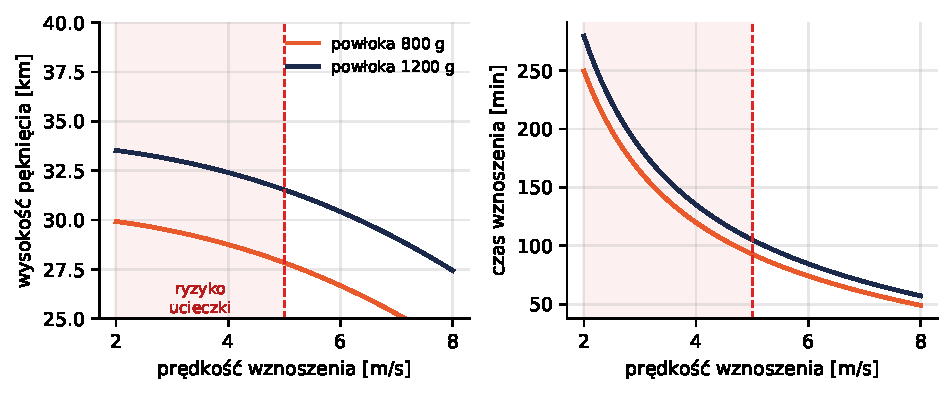
\includegraphics[width=\linewidth]{heurystyka_wznoszenia}\end{center}
\captionof{figure}{Wysokość pęknięcia i czas wznoszenia w funkcji prędkości wznoszenia. Obliczenia metodą kalkulatora SondeHub~\cite{sondehubcalc} dla ładunku \SI{2}{kg}. Obszar czerwony: ryzyko ucieczki.}\label{fig:heurystyka}
\end{sekcja}

\begin{sekcja}{Obliczenie ilości gazu}
\begin{enumerate}
  \item Zważ cały zestaw lotny bez powłoki.
  \item Otwórz kalkulator SondeHub: \url{https://sondehub.org/calc/}.
  \item Wpisz masę ładunku. Wybierz model powłoki.
  \item Wpisz docelową prędkość wznoszenia: \SI{5}{m/s}.
  \item Zapisz w karcie misji (F0): siłę nośną szyjki (\emph{neck lift}), objętość gazu, wysokość pęknięcia, czas do pęknięcia.
  \item Zamów gaz z zapasem co najmniej \SI{30}{\percent} (straty, powtórka, butla z mniejszą ilością gazu).
\end{enumerate}

\small
\begin{tabularx}{\linewidth}{@{}YYYYY@{}}
\toprule
\textbf{Wznoszenie [m/s]} & \textbf{Gaz [m³]} & \textbf{Siła nośna szyjki [kg]} & \textbf{Pęknięcie [km]} & \textbf{Wznoszenie [min]}\\\midrule
\wiersze{figures/generated/tabela_wznoszenia.tex}
\bottomrule
\end{tabularx}
\normalsize
\captionof{table}{Przykład: ładunek \SI{2}{kg}, powłoka \SI{800}{g} (średnica pęknięcia \SI{7}{m}). Tylko do orientacji -- dla swojej misji użyj kalkulatora.}
\end{sekcja}

\begin{sekcja}{Predykcja trajektorii}
\begin{enumerate}
  \item Otwórz predyktor SondeHub: \url{https://predict.sondehub.org/}.
  \item Wpisz miejsce startu, datę i godzinę, prędkość wznoszenia, wysokość pęknięcia i prędkość opadania.
  \item Sprawdź miejsce lądowania.
  \item Powtarzaj predykcję codziennie od około 7 dni przed lotem. Wpisuj wyniki do dziennika predykcji (formularz F4). Prognoza wiatru się zmienia.
  \item Wybierz termin i miejsce, dla których miejsce lądowania jest bezpieczne i dostępne.
\end{enumerate}
\end{sekcja}

\begin{sekcja}{Scenariusze zapasowe}
Po wysłaniu zgłoszenia do PAŻP nie możesz zmienić miejsca ani godziny startu. Dlatego:
\begin{itemize}
  \item wyślij \textbf{dwa zgłoszenia}: dla miejsca zasadniczego i dla miejsca zapasowego,
  \item w każdym zgłoszeniu podaj termin zasadniczy i termin zapasowy, np. 1--2 godziny po pierwszej godzinie albo inny dzień,
  \item przygotuj \textbf{plan działania dla każdego scenariusza}: kto jedzie gdzie, kiedy zespół decyduje, co robi, gdy żaden scenariusz nie jest bezpieczny.
\end{itemize}

\renewcommand{\arraystretch}{1.6}
\begin{tabularx}{\linewidth}{@{}|P{12mm}|L|L|L|@{}}\hline
\textbf{Scen.} & \textbf{Miejsce i godzina} & \textbf{Warunek wyboru} & \textbf{Plan działania}\\\hline
A & & & \\\hline
B & & & \\\hline
C & & & \\\hline
\end{tabularx}
\end{sekcja}

\begin{sekcja}{Kryteria braku startu}
\textbf{Nie startuj}, gdy predykcja pokazuje lądowanie:
\begin{itemize}
  \item w morzu, jeziorze albo na rozległym terenie podmokłym,
  \item w dużym lesie albo w mieście,
  \item w strefie kontrolowanej lotniska,
  \item za granicą państwa -- w szczególności w Rosji (obwód kaliningradzki), na Białorusi i na Ukrainie. Lot nad tymi państwami jest niedopuszczalny ze względu na sytuację geopolityczną. Odzyskanie ładunku jest tam niemożliwe, a lot może zostać uznany za incydent.
\end{itemize}

\textbf{Nie startuj}, gdy:
\begin{itemize}
  \item wiatr przy ziemi jest silny (tankowanie i start są niebezpieczne),
  \item pada deszcz, jest burza albo niska podstawa chmur,
  \item test trackera na stanowisku nie przeszedł (brak pozycji GPS albo brak odbioru telemetrii),
  \item którykolwiek punkt przeglądu gotowości (formularz F6) jest niespełniony.
\end{itemize}
\end{sekcja}

\begin{sekcja}{Wymagane testy}\label{sec:testy}
Wykonaj te testy przed każdą misją, dla platformy i dla każdego ładunku. Zapisz wyniki w formularzu F5.

\renewcommand{\arraystretch}{1.3}
\small
\begin{tabularx}{\linewidth}{@{}P{38mm}LP{30mm}@{}}
\toprule
\textbf{Test} & \textbf{Jak} & \textbf{Kryterium}\\\midrule
Funkcjonalny & Wszystkie funkcje na stole, z zasilania bateryjnego. & Wszystko działa.\\
W zimnie & Zamrażarka (\SI{-20}{\degreeCelsius}) albo zamrażarka laboratoryjna (\SI{-80}{\degreeCelsius}) przez czas lotu, urządzenia włączone. & Działa, zapisuje dane.\\
Zasięg radia & Tracker z anteną lotną; odbiór z odległości co najmniej \SI{100}{m}, najlepiej kilku km. & Pakiety odebrane, pozycja na mapie.\\
Odcinacz & Zwolnienie pod pełnym obciążeniem, ze skręconymi linkami, po schłodzeniu. & 10 z 10 prób.\\
Czas pracy & Cały system na bateriach lotnych. & $\geq 2\times$ czas lotu + czas poszukiwań.\\
Upadek & Gondola zrzucona z około \SI{1}{m} na twarde podłoże. & Nic się nie odłącza.\\
Próba generalna & Cały montaż i formularze dnia startu, bez balonu. & Zespół zna role i kolejność.\\
\bottomrule
\end{tabularx}
\normalsize

\begin{wskazowka}Zapytaj biologów na Wydziale Chemicznym, czy możesz użyć ich zamrażarki laboratoryjnej. Zamrażarki do przechowywania próbek osiągają \SI{-80}{\degreeCelsius} -- warunki bliższe stratosferze niż domowa zamrażarka.\end{wskazowka}
\end{sekcja}

\begin{sekcja}{Przegląd gotowości do startu}
Kilka dni przed lotem zespół robi przegląd gotowości (\emph{Flight Readiness Review}). Kierownik misji przechodzi z zespołem przez formularz F6. Każdy punkt ma dowód: wynik testu, potwierdzenie z PAŻP, zdjęcie, wpis w karcie misji.

Wynik przeglądu to decyzja „leci / nie leci”. Brak dowodu oznacza „nie leci”, dopóki zespół go nie dostarczy.
\end{sekcja}

\chapter{Wymagania prawne}\label{ch:prawo}

\begin{uwaga}Przepisy i formularze się zmieniają. Przed każdą misją sprawdź aktualne wymagania na stronach PAŻP i w tekście rozporządzenia SERA.\end{uwaga}

\begin{sekcja}{Klasyfikacja balonu (SERA)}
Loty bezzałogowych balonów wolnych reguluje rozporządzenie wykonawcze Komisji (UE) nr 923/2012 (SERA), Dodatek~2~\cite{sera}. Klasa balonu określa wymagania. Określ klasę przed wypełnieniem zgłoszenia.

\renewcommand{\arraystretch}{1.35}
\begin{tabularx}{\linewidth}{@{}P{20mm}L@{}}
\toprule
\textbf{Klasa} & \textbf{Kryteria}\\\midrule
Lekki & Łączna masa ładunku mniejsza niż \SI{4}{kg} (jeżeli nie spełnia kryteriów balonu ciężkiego).\\
Średni & Dwa lub więcej pakietów o łącznej masie od \SI{4}{kg} do mniej niż \SI{6}{kg}.\\
Ciężki & Co najmniej jeden warunek: łączna masa \SI{6}{kg} lub więcej; jeden pakiet \SI{3}{kg} lub więcej; pakiet \SI{2}{kg} lub więcej o gęstości powierzchniowej większej niż \SI{13}{g/cm^2}; linka lub urządzenie podwieszenia, które wymaga siły \SI{230}{N} lub więcej, aby oddzielić ładunek od balonu.\\
\bottomrule
\end{tabularx}

Gęstość powierzchniowa = masa pakietu [g] / pole najmniejszej ściany pakietu [cm²].

\textbf{Zalecenia projektowe:}
\begin{itemize}
  \item Projektuj zestaw jako balon \textbf{lekki}. Wymagania dla balonu ciężkiego (dwa niezależne systemy zakończenia lotu, transponder, oświetlenie, raportowanie pozycji) są trudne do spełnienia dla zespołu studenckiego.
  \item Użyj linki, która zrywa się przy sile mniejszej niż \SI{230}{N} -- w praktyce linka o średnicy około \SI{1}{mm}. Sprawdź wytrzymałość w karcie katalogowej albo wykonaj odpowiedni test (np. zerwij próbkę linki, mierząc siłę wagą bagażową).
  \item Podziel ładunek na pakiety o masie poniżej \SI{2}{kg}.
\end{itemize}
\end{sekcja}

\begin{sekcja}{Zgłoszenie lotu do PAŻP}
Polska Agencja Żeglugi Powietrznej (PAŻP) przyjmuje zgłoszenia sondowań atmosfery i publikuje ostrzeżenie dla pilotów (NOTAM)~\cite{pazp}.

\textbf{Formularz:} formularz zgłoszenia sondowania atmosfery (ASM1):\\
\url{https://www.pansa.pl/wp-content/uploads/2025/07/Formularz_sonda_v1.pdf}\\
Lista aktualnych formularzy: \url{https://www.pansa.pl/asm1/formularze-zgloszeniowe/}

\textbf{Procedura:}
\begin{enumerate}
  \item Sprawdź strefy przestrzeni powietrznej w miejscu startu i na przewidywanej trasie lotu (rozdział~\ref{ch:planowanie}, sekcja~\ref{sec:strefy}).
  \item Pobierz aktualny formularz (adres wyżej). Sprawdź, czy PAŻP nie opublikowała nowej wersji.
  \item Wypełnij \textbf{dwa formularze}: dla miejsca zasadniczego i zapasowego. W każdym podaj termin zasadniczy i zapasowy (rozdział~\ref{ch:planowanie}).
  \item Wyślij formularze e-mailem do działu ASM1: \texttt{asm1@pansa.pl}, co najmniej 14 dni przed lotem. Minimalny termin podaje strona PAŻP -- sprawdź go przed każdą misją. Dział ASM1 pracuje w dni robocze.
  \item Zapisz w karcie misji (F0) numer zgłoszenia i numer telefonu do służby ruchu lotniczego z odpowiedzi PAŻP.
  \item Przed startem sprawdź w AIS Polska, czy NOTAM dla misji jest opublikowany.
  \item W dniu startu miej numer do służby ruchu lotniczego pod ręką. Gdy zmienisz plan (godzina, odwołanie), zadzwoń natychmiast.
\end{enumerate}
\end{sekcja}

\begin{sekcja}{Dane w formularzu PAŻP}
\renewcommand{\arraystretch}{1.3}
\begin{tabularx}{\linewidth}{@{}P{26mm}L@{}}
\toprule
\textbf{Sekcja} & \textbf{Dane}\\\midrule
Organizator & Imię i nazwisko, telefon, e-mail.\\
Termin & Termin zasadniczy i zapasowy: data, godziny (UTC), planowana godzina startu.\\
Lokalizacja & Nazwa miejscowości, współrzędne WGS-84 (stopnie, minuty, sekundy).\\
Balon & Kolor, ilość, klasa (lekki/średni/ciężki), masa powłoki, wysokość sondowania, prędkość wznoszenia i opadania, średnica przy starcie i na wysokości pęknięcia.\\
Ładunek & Kolor i średnica spadochronu, kolor ładunku, częstotliwość nadajnika, masa ładunku ze spadochronem, gęstość powierzchniowa (gdy pakiet ma \SI{2}{kg} lub więcej).\\
Opis & Krótki opis przedsięwzięcia.\\
\bottomrule
\end{tabularx}

Dane o średnicy, wysokości i prędkości weź z kalkulatora (rozdział~\ref{ch:planowanie}).
\end{sekcja}

\begin{sekcja}{Licencja radiowa}
Nadajniki trackera (APRS na \SI{144.8}{MHz}, RTTY na \SI{434}{MHz}) wymagają pozwolenia radiowego dla służby amatorskiej. Operator z licencją krótkofalowca odpowiada za nadajnik i udostępnia swój znak wywoławczy.

\begin{itemize}
  \item Jak zdobyć licencję krótkofalowca w Polsce (egzamin, pozwolenie, znak): przewodnik Hackerspace Kraków~\cite{faqradiowe}: \url{https://github.com/HackerspaceKRK/faq-radiowe}.
  \item Sprawdź, czy warunki pozwolenia dopuszczają pracę z balonu. Niektóre kraje zabraniają APRS w powietrzu.
  \item Moduły ISM (np. \SI{434}{MHz}, LoRa) mają limity mocy i cyklu pracy. Sprawdź je dla użytego pasma.
\end{itemize}

\begin{wskazowka}Zdobądź licencję w zespole z wyprzedzeniem -- egzamin i wydanie pozwolenia trwają tygodnie.\end{wskazowka}
\end{sekcja}

\begin{sekcja}{Znak wywoławczy misji}
Każda misja nadaje pod znakiem wywoławczym konkretnej osoby albo klubu. Właściciel znaku odpowiada za nadajnik.

Kolejność wyboru znaku:
\begin{enumerate}
  \item \textbf{Znak klubowy SimLE} -- docelowo koło ma własny klubowy znak krótkofalarski.\par
  {\raggedright\pole[45mm]{Znak klubowy:}\par\pole[45mm]{Osoba odpowiedzialna:}\par}
  \item \textbf{Znak członka zespołu} z licencją krótkofalowca.
  \item \textbf{Znak udostępniony przez osobę spoza zespołu} -- tylko za jej wyraźną zgodą.
\end{enumerate}

\begin{uwaga}[Znak SR0FLY]Znak SR0FLY, używany w misji z 27.02.2022, należy do Macieja Jakimca (Fundacja Copernicus Project, nearspace.pl). Przed każdym użyciem tego znaku \textbf{bezwzględnie} skontaktuj się z nim i poproś o zgodę:\\
\url{https://nearspace.pl/pl/cms/o-nas-30.html}\\
\url{https://nearspace.pl/pl/contact.html}\end{uwaga}

Zapisz w karcie misji (F0): znak, SSID, właściciela znaku i datę jego zgody.
\end{sekcja}

\begin{sekcja}{Ubezpieczenie OC}
Wykup ubezpieczenie odpowiedzialności cywilnej na lot.
\begin{itemize}
  \item Zespół KSat e.V. z Uniwersytetu w Stuttgarcie, który prowadzi własne misje balonowe (projekt BUBBLE)~\cite{ksat}, rekomenduje lotnicze ubezpieczenie OC firmy Allianz według ogólnych warunków AMU~300/06~\cite{amu}.
  \item Sprawdź, czy polisa obejmuje bezzałogowe balony wolne. Ogólne polisy lotnicze często nie wymieniają balonów wprost.
  \item W Polsce: zapytaj ubezpieczyciela uczelni albo brokera o OC organizacji z klauzulą lotniczą. Podaj klasę balonu, masę ładunku i obszar lotu.
\end{itemize}
\end{sekcja}

\begin{sekcja}{Oznakowanie ładunku}
Opisz każdy pakiet. Wystarczy pisać markerem permanentnym bezpośrednio na styropianie.
\begin{itemize}
  \item \textbf{Numer telefonu -- obowiązkowo.} Osoba, która znajdzie gondolę, musi móc zadzwonić.
  \item Informacja dla osób postronnych (zalecana): „Projekt badawczy -- nie otwierać, prosimy o kontakt”.
  \item Logo projektu (naklejka) -- zwiększa zaufanie znalazcy.
  \item Ostrzeżenia, np. o bateriach litowych.
\end{itemize}

\dwafoto{2023_gondola_bok_termometr}{Oznakowanie markerem: „Projekt badawczy”. Z boku wyprowadzony czujnik temperatury.}
{2023_gondole_po_locie}{Numer telefonu („Znalazłeś? Zadzwoń!” -- numer zamazany w tej publikacji), napis „Projekt badawczy” i naklejki z logo misji.}
\end{sekcja}

\chapter{Segment naziemny}\label{ch:naziemny}

\begin{sekcja}{Stanowisko startowe}
Wybierz otwarty teren bez drzew i linii energetycznych, np. boisko. Uzyskaj zgodę właściciela terenu. Powłoka jest delikatna: gałązki, korzenie i kamienie mogą ją przebić.

Rysunek~\ref{fig:stanowisko} pokazuje warstwy stanowiska. Powłoka leży \textbf{między dwiema foliami}. Tankowanie odbywa się między foliami. Folia górna przytrzymuje powłokę, aby nie odleciała przed startem.

\begin{center}\resizebox{\linewidth}{!}{\rysStanowisko}\end{center}
\captionof{figure}{Przekrój stanowiska startowego (grubość warstw przesadzona).}\label{fig:stanowisko}
\end{sekcja}

\begin{sekcja}{Warstwy stanowiska}
\begin{enumerate}
  \item \textbf{Plandeka} -- na sam dół. Chroni przed wilgocią z ziemi. Jest ważna przy starcie rano, gdy trawa jest mokra.
  \item \textbf{Koc} -- chroni powłokę przed przebiciem przez korzenie i odrosty. Gruby koc działa lepiej niż cienki.
  \item \textbf{Folia malarska dolna} (cienka) -- pod powłoką.
  \item \textbf{Powłoka} i rura do tankowania.
  \item \textbf{Folia malarska górna} (grubsza) -- na powłoce. Cienka folia na wierzchu może się porwać i powłoka może odlecieć w trakcie tankowania. Grubsza folia jest pewniejsza.
\end{enumerate}

\begin{uwaga}Dociśnij rogi plandeki, koca i folii czymś ciężkim, np. skrzynkami transportowymi. Porywy wiatru mogą porwać folię razem z powłoką.\end{uwaga}

\begin{wskazowka}Folię, plandekę i koce kupisz w markecie budowlanym. Kup oba rodzaje folii, aby mieć wybór. Kup wszystko na jeden rachunek razem z zamówieniem gazu -- upraszcza to rozliczenie.\end{wskazowka}
\end{sekcja}

\begin{sekcja}{Stanowisko na zdjęciach}
\dwafoto{2023_stanowisko_rozlozone}{Rozłożona plandeka i sprzęt przed tankowaniem.}
{2023_powloka_miedzy_foliami}{Powłoka na folii dolnej; pomocnicy przykrywają ją folią górną.}
\dwafoto{2022_stanowisko_zabezpieczone}{Rogi folii dociśnięte skrzynkami transportowymi.}
{2023_balon_po_tankowaniu}{Zatankowana powłoka trzymana folią górną do chwili startu.}
\end{sekcja}

\begin{sekcja}{Sprzęt do tankowania}
\begin{itemize}
  \item butla z helem (zwykle \SI{50}{l}, \SI{200}{bar}) i reduktor z dwoma manometrami,
  \item wąż i rura do tankowania (najlepiej z zaworem zwrotnym),
  \item obciążnik o masie równej sile nośnej szyjki -- dla ładunku do \SI{4}{kg} to kilka kilogramów: worek z piaskiem, plecak z obciążeniem albo odważniki (butelka z wodą jest za lekka),
  \item waga bagażowa (zakres do kilkunastu kilogramów) do ważenia obciążnika i zestawu,
  \item klucz do reduktora: klucz nastawny („francuski”) albo klucze calowe -- zależnie od butli,
  \item taśma klejąca (mocna, np. srebrna), sznurek, opaski zaciskowe,
  \item rękawiczki (bawełniane albo nitrylowe) dla wszystkich, którzy dotykają powłoki,
  \item termometry do pomiaru temperatury butli i powietrza (sekcja~\ref{sec:temp-butli}): pirometr, czarna matowa taśma izolacyjna, termometr pogodowy, opcjonalnie termometr kontaktowy,
  \item czujnik wodoru -- na wszelki wypadek, gdy gaz w butli może zawierać wodór albo gdy zespół używa wodoru.
\end{itemize}

\begin{uwaga}Pracuj przy powłoce tylko w rękawiczkach. Tłuszcz ze skóry osłabia lateks. Powłoka pęka wcześniej w miejscach, które ktoś dotknął gołą ręką.\end{uwaga}

\begin{uwaga}Butla z gazem pod ciśnieniem \SI{200}{bar} jest niebezpieczna~\cite[rozdz.~6]{nasahb}:
\begin{itemize}
  \item Transportuj ją zabezpieczoną przed przetoczeniem (rozdział~\ref{ch:planowanie}). Nie upuszczaj jej i nie uderzaj.
  \item Nie tocz i nie ciągnij butli. Na krótkie odległości przewoź ją na wózku.
  \item Nie dopuszczaj do nagrzania powyżej \SI{50}{\degreeCelsius}: nie zostawiaj butli w samochodzie na słońcu.
  \item Nie zdejmuj kołpaka z zaworu, dopóki butla nie leży stabilnie na stanowisku.
  \item Nie otwieraj zaworu bez zamontowanego reduktora.
  \item Przed misją obejrzyj wąż, reduktor i uszczelki. Nie zginaj węża na ostro -- zagięcie osłabia go niewidocznie.
\end{itemize}\end{uwaga}

\begin{uwaga}[Transport butli]Przewóz butli z gazem sprężonym podlega przepisom o przewozie towarów niebezpiecznych (ADR) i może wymagać uprawnień. Jeżeli procedury zakupowe na to pozwalają, kup albo wypożycz butlę u dostawcy blisko miejsca startu i odbierz ją na miejscu.\end{uwaga}
\end{sekcja}

\begin{sekcja}{Przygotowanie reduktora}
Reduktor ma dwa manometry:
\begin{itemize}
  \item \textbf{manometr wysokiego ciśnienia} (ciśnienie w butli, skala do ok. \SI{300}{bar}) -- z niego odczytujesz $p_1$ i $p_2$,
  \item \textbf{wskaźnik przepływu} (skala w l/min, skalowana dla argonu i CO$_2$) -- do ustawienia i utrzymania stałego przepływu.
\end{itemize}

\begin{enumerate}
  \item Połóż butlę stabilnie na plandece, w cieniu. Zabezpiecz ją przed przetoczeniem. Naklej na butlę kawałek czarnej taśmy do pomiaru temperatury (sekcja~\ref{sec:temp-butli}).
  \item Sprawdź gwint zaworu butli i reduktora. Usuń zanieczyszczenia.
  \item Przykręć reduktor kluczem. Nie dokręcaj na siłę.
  \item Zamknij pokrętło reduktora (pozycja \emph{OFF}). Otwórz powoli zawór butli.
  \item Odczytaj z \textbf{manometru wysokiego ciśnienia} ciśnienie początkowe $p_1$ (bez przepływu -- reduktor zamknięty). Zmierz temperaturę butli $T_1$. Zapisz obie wartości w formularzu F10.
  \item Sprawdź szczelność: zamknij zawór butli. Ciśnienie na manometrze wysokiego ciśnienia nie może spadać.
  \item Podłącz wąż i rurę do tankowania.
\end{enumerate}

\dwafoto{2022_regulator_montaz}{Montaż reduktora na butli -- w rękawiczkach, na plandece.}
{2022_regulator_manometry}{Manometry reduktora: górny -- ciśnienie w butli [bar], dolny -- przepływ [l/min], skalowany dla argonu i CO$_2$.}
\end{sekcja}

\begin{sekcja}{Ilość gazu z ciśnienia w butli}\label{sec:gaz-wzor}
Manometr wysokiego ciśnienia pokazuje ciśnienie w butli. Ze spadku ciśnienia obliczysz, ile gazu poszło do powłoki. Wzór wynika z równania stanu gazu z poprawką na ściśliwość helu~\cite{nist}, \cite[rozdz.~6]{nasahb}:
\[
  V \;=\; \frac{V_b\,T_0}{p_0}\left(\frac{p_1}{Z(p_1)\,T_1} - \frac{p_2}{Z(p_2)\,T_2}\right),
  \qquad Z(p) \approx 1 + 4{,}8\cdot10^{-4}\,p\ [\text{bar}]
\]
gdzie:
\begin{itemize}
  \item $V$ -- objętość helu wypuszczonego do powłoki, przy ciśnieniu atmosferycznym [m³],
  \item $V_b$ -- pojemność wodna butli (wybita na butli, np. \SI{50}{l} = \SI{0.05}{m^3}),
  \item $p_1$, $p_2$ -- ciśnienie \textbf{bezwzględne} przed i po tankowaniu: odczyt manometru wysokiego ciśnienia + \SI{1}{bar}; odczytuj tylko przy zamkniętym zaworze -- w czasie przepływu manometr pokazuje za mało,
  \item $p_0 = \SI{1.013}{bar}$ -- ciśnienie atmosferyczne,
  \item $Z$ -- współczynnik ściśliwości helu (dla \SI{200}{bar} $Z \approx 1{,}1$; bez poprawki wynik jest zawyżony o około \SI{10}{\percent}),
  \item $T_1$, $T_2$ -- temperatura gazu w butli [K] przy odczycie $p_1$ i $p_2$ (sekcja~\ref{sec:temp-butli}); $T_0 = \SI{288}{K}$. Błąd temperatury \SI{10}{\degreeCelsius} to błąd ilości gazu około \SI{3.5}{\percent}.
\end{itemize}

Siła nośna helu przy ziemi to około \SI{1.05}{kg} na każdy \si{m^3}. Siła nośna szyjki = $V \cdot 1{,}05$~kg $-$ masa powłoki.
\end{sekcja}

\begin{sekcja}{Tabela gazu}
\small
\begin{tabularx}{\linewidth}{@{}YYYYY@{}}
\toprule
\makecell{\textbf{Odczyt}\\\textbf{manometru [bar]}} & \makecell{\textbf{Spadek}\\\textbf{ciśnienia [bar]}} & \makecell{\textbf{Hel z butli}\\\textbf{10 l [m³]}} & \makecell{\textbf{Hel z butli}\\\textbf{50 l [m³]}} & \makecell{\textbf{Siła nośna}\\\textbf{(50 l) [kg]}}\\\midrule
\wiersze{figures/generated/tabela_gazu.tex}
\bottomrule
\end{tabularx}
\normalsize
\captionof{table}{Hel wypuszczony z butli napełnionej do \SI{200}{bar}, w temperaturze \SI{15}{\degreeCelsius}. Pełna butla \SI{50}{l} zawiera około \SI{9}{m^3} helu. Reguła: z butli \SI{50}{l} każde \SI{10}{bar} spadku to około 0,4--0,5~m³ helu.}\label{tab:gaz}

\begin{uwaga}Przy szybkim wypływie butla się ochładza i manometr pokazuje za niskie ciśnienie. Przed odczytem $p_2$ zamknij zawór i odczekaj kilka minut, aż temperatura się wyrówna.\end{uwaga}

Hel balonowy („balloon gas”) bywa mieszaniną helu z powietrzem. Ma mniejszą siłę nośną. Zamów hel techniczny o czystości podanej przez dostawcę i zapisz ją w karcie misji.
\end{sekcja}

\begin{sekcja}{Pomiar temperatury butli}\label{sec:temp-butli}
Termometr mierzy temperaturę \textbf{ścianki} butli, nie gazu. Ścianka i gaz mają tę samą temperaturę tylko w równowadze: butla stoi długo w stałej temperaturze, w cieniu, a gaz nie płynie~\cite[rozdz.~6]{nasahb}. W czasie wypływu gaz w butli się ochładza, a słońce nagrzewa ściankę -- pomiar jest wtedy fałszywy.

\textbf{Przygotowanie:} od przyjazdu trzymaj butlę w cieniu (albo przykrytą jasnym materiałem). Naklej na butlę, na wysokości połowy, kawałek \textbf{czarnej matowej taśmy izolacyjnej PVC} (około 5$\times$\SI{5}{cm}). Taśma ma znaną emisyjność $\varepsilon \approx 0{,}95$. Naklej ją kilka minut przed pomiarem, aby przyjęła temperaturę butli.

\textbf{Pirometr} (termometr na podczerwień) -- metoda podstawowa:
\begin{enumerate}
  \item Ustaw w pirometrze emisyjność $\varepsilon = 0{,}95$ (wiele tanich pirometrów ma ją ustawioną na stałe).
  \item Celuj w taśmę, nie w gołą butlę. Goły lub błyszczący metal ma małą i nieznaną emisyjność: odbija promieniowanie otoczenia i pirometr pokazuje fałszywą wartość.
  \item Podejdź tak blisko, aby plamka pomiaru była mniejsza niż taśma. Przy pirometrze 12:1 z odległości \SI{12}{cm} plamka ma około \SI{1}{cm}.
  \item Zmierz trzy razy i zapisz średnią.
\end{enumerate}

\textbf{Termometr kontaktowy} (sonda powierzchniowa, np. termopara typu K z multimetrem) -- kontrola: dociśnij sondę do butli, przykryj ją kawałkiem pianki albo rękawiczką i odczekaj, aż odczyt się ustali.

\textbf{Termometr pogodowy} -- temperatura powietrza w cieniu. Gdy butla stała kilka godzin na zewnątrz w cieniu, jej temperatura jest bliska temperaturze powietrza. Duża różnica oznacza błąd pomiaru albo butlę nagrzaną w samochodzie.

\textbf{Kiedy mierzyć:} $T_1$ -- przed otwarciem reduktora, razem z $p_1$. $T_2$ -- po zamknięciu zaworu i odczekaniu kilku minut, razem z $p_2$. Zapisz obie wartości i temperaturę powietrza w formularzu F10.
\end{sekcja}

\begin{sekcja}{Hel czy wodór}\label{sec:hel-wodor}
Zespół wybiera gaz na etapie planowania misji (sekcja~\ref{sec:powloka}). Platforma Stardust NEXT używa \textbf{helu}. Hel drożeje i bywa trudno dostępny, dlatego część zespołów balonowych przechodzi na wodór~\cite[rozdz.~2]{nasahb}. Wodór daje około \SI{10}{\percent} więcej siły nośnej, ale jest palny i wymaga dodatkowego szkolenia.

\begin{uwaga}Nowym zespołom nie zalecamy wodoru. Jeśli zespół mimo to wybierze wodór, stosuj zasady z rozdziału~6 podręcznika NASA~\cite{nasahb}:
\begin{itemize}
  \item żadnego ognia, iskier ani testów elektroniki przy butli i przy powłoce; silniki samochodów wyłączone,
  \item uziem butlę i sprzęt, zanim wypuścisz gaz,
  \item odzież z bawełny, nie z tworzyw sztucznych,
  \item przed tankowaniem wyznacz strefę zagrożenia: owal wzdłuż wiatru, balon przy jego nawietrznym końcu. Uciekaj pod wiatr, gdy stoisz po nawietrznej; z innych miejsc -- w poprzek wiatru. Nigdy nie przechodź przez oś owalu,
  \item płomień wodoru jest niewidoczny. Ktoś z zewnątrz strefy obserwuje stanowisko i ostrzega,
  \item resztki powłoki po locie mogą zawierać kieszenie gazu -- nie zostawiaj ich bez nadzoru.
\end{itemize}
Wzór i tabela gazu w tym rozdziale dotyczą tylko helu.\end{uwaga}
\end{sekcja}

\begin{sekcja}{Ilość gazu z przepływu i czasu}
Operator butli może szacować ilość gazu na bieżąco: ustaw \textbf{stały przepływ} na wskaźniku przepływu i mierz czas.

Wskaźnik przepływu jest skalowany dla argonu. Hel jest około 10 razy lżejszy, więc rzeczywisty przepływ helu jest około \textbf{3 razy większy} niż wskazanie ($\sqrt{40/4} \approx 3{,}2$).

\textbf{Reguła inżynierska:}
\[
  t\,[\text{min}] \;\approx\; \frac{310 \cdot V\,[\text{m}^3]}{Q_\text{wsk}\,[\text{l/min}]}
\]
Przykład: przy wskazaniu \SI{30}{l/min} tankowanie trwa około \textbf{10 minut na każdy m³} helu.

\renewcommand{\arraystretch}{1.25}
\small
\begin{tabularx}{\linewidth}{@{}YYYY@{}}
\toprule
\textbf{Wskazanie [l/min]} & \textbf{Hel rzeczywiście [l/min]} & \textbf{Czas na 1 m³ [min]} & \textbf{Czas na 3 m³ [min]}\\\midrule
10 & ok. 32 & 31 & 93\\
20 & ok. 63 & 16 & 47\\
30 & ok. 95 & 10 & 31\\
\bottomrule
\end{tabularx}
\normalsize

To zgrubne oszacowanie: wskazanie zależy od reduktora i od ciśnienia za nim. Co kilka minut porównuj je ze spadkiem ciśnienia w butli (tabela~\ref{tab:gaz}). O końcu tankowania decyduje metoda z obciążnikiem.
\end{sekcja}

\begin{sekcja}{Metoda z obciążnikiem}
Metoda z obciążnikiem to podstawowa metoda tankowania. Wzory służą do kontroli i do oceny, ile gazu zostało w butli.
\begin{enumerate}
  \item Odczytaj z kalkulatora siłę nośną szyjki (\emph{neck lift}).
  \item Przygotuj obciążnik o masie równej \textbf{sile nośnej szyjki z kalkulatora} (worek z piaskiem, plecak, odważniki). Uwzględnij masę rury do tankowania i taśmy, jeśli wiszą razem z obciążnikiem. Zważ obciążnik wagą bagażową.
  \item Przywiąż obciążnik do szyjki albo do rury do tankowania.
  \item Tankuj, aż balon \textbf{uniesie obciążnik} (balon w równowadze albo lekko się wznosi).
\end{enumerate}

\begin{uwaga}Masa obciążnika to siła nośna szyjki z kalkulatora, \textbf{nie} masa gondoli ze zgłoszenia do PAŻP. Siła nośna szyjki = masa zestawu + nadwyżka siły nośnej, która daje prędkość wznoszenia. Balon zatankowany „na masę gondoli” prawie nie ma nadwyżki: wyrwie się z rąk, a potem będzie się wlókł nisko -- po budynkach, liniach energetycznych i drzewach. To skrajnie niebezpieczne.\end{uwaga}

\begin{center}\resizebox{\linewidth}{!}{\rysTankowanie}\end{center}
\captionof{figure}{Tankowanie metodą z obciążnikiem.}
\end{sekcja}

\begin{sekcja}{Procedura tankowania}
\begin{enumerate}
  \item Wszyscy przy powłoce zakładają rękawiczki.
  \item Wyjmij powłokę z opakowania na folii dolnej. Rozłóż ją bez naciągania.
  \item Włóż rurę do tankowania w szyjkę powłoki. Owiń szyjkę dookoła rury i przytrzymaj ręką.
  \item Wstępnie uszczelnij szyjkę na rurze taśmą -- \textbf{delikatnie}, tak aby dało się ją zdjąć.
  \item Przykryj powłokę folią górną. Pomocnicy trzymają brzegi folii.
  \item Otwórz zawór butli i powoli otwieraj reduktor. Ustaw stały przepływ. Zapisz godzinę.
  \item Obserwuj manometr wysokiego ciśnienia. Zapisuj odczyty (formularz F10). Porównuj z tabelą~\ref{tab:gaz} i z czasem tankowania.
  \item Gdy balon uniesie obciążnik, zamknij zawór butli. Sprawdź siłę nośną jeszcze raz po minucie.
  \item Po kilku minutach odczytaj $p_2$ i zmierz temperaturę butli $T_2$ (formularz F10).
  \item Zamknij powłokę (sekcja~\ref{sec:szyjka}).
\end{enumerate}

\dwafoto{2023_tankowanie_rura}{Tankowanie: szyjka owinięta dookoła rury i przytrzymana ręką. Pętla olinowania z krętlikiem gotowa. Taśma w gotowości na plandece.}
{2020_tankowanie_torun}{Tankowanie pod folią (20.07.2020).}
\end{sekcja}

\begin{sekcja}{Zamknięcie powłoki}\label{sec:szyjka}
Przygotuj wcześniej pętlę olinowania z krętlikiem. Pętla jest gotowa do założenia zaraz po tankowaniu.
\begin{enumerate}
  \item Zdejmij taśmę wstępną. Wysuń rurę z szyjki, trzymając szyjkę zaciśniętą w dłoni.
  \item Skręć szyjkę kilka razy.
  \item Przewiąż skręconą szyjkę sznurkiem. Zrób kilka supłów.
  \item Przełóż przez szyjkę przygotowaną pętlę olinowania (z krętlikiem), \textbf{przed} zgięciem szyjki.
  \item Zegnij szyjkę w pół \textbf{w górę} (w stronę powłoki). Pętla zostaje w zgięciu.
  \item Zaciśnij zgiętą szyjkę kilkoma opaskami zaciskowymi.
  \item Owiń całość kilkoma warstwami taśmy.
  \item Pociągnij za pętlę: pętla nie może się zsunąć z szyjki.
\end{enumerate}

Zamknięcie musi być \textbf{szczelne}. Szczelności nie da się łatwo sprawdzić na stanowisku -- zdaj się na intuicję inżynierską: wiąż mocno, nie żałuj supłów, opasek i taśmy. Nieszczelna szyjka to wolniejsze wznoszenie, niższy pułap albo lot bez pęknięcia.

\begin{uwaga}Nie przyklejaj taśmy do powłoki. Taśma odklejana od powłoki może ją przerwać. Taśma ma dotykać tylko szyjki.\end{uwaga}
\end{sekcja}

\begin{sekcja}{Stacje odbiorcze}
Używaj co najmniej dwóch stacji odbiorczych: stacjonarnej i mobilnej. Nie polegaj tylko na sieci innych nasłuchowców. Schemat toru radiowego: rozdział~\ref{ch:elektronika}.

\textbf{Stacja stacjonarna:} antena kierunkowa albo dookólna na wysokim maszcie, odbiornik SDR i komputer z internetem. Stacja wysyła odebrane pakiety do SondeHub i APRS-IS.

\textbf{Stacja mobilna}, wariant 1: radiotelefon z dekoderem APRS (np. Yaesu FT5DE) i antena samochodowa VHF/UHF na magnes (np. Nagoya UT-72).

\textbf{Stacja mobilna}, wariant 2: odbiornik RTL-SDR, przedwzmacniacz niskoszumny (LNA), filtry pasmowe, laptop z oprogramowaniem dekodującym.

\begin{wskazowka}[APRS bez dekodera]Tani radiotelefon bez dekodera APRS (np. Baofeng) też wystarczy. Połącz wyjście audio radia z telefonem albo laptopem (kabel audio albo adapter Bluetooth). Dekoduj APRS aplikacją APRSdroid (Android) albo programem Direwolf (laptop).\end{wskazowka}

\foto[0.6\linewidth]{2022_poscig_samochod}{Stacja mobilna w samochodzie pościgowym: laptop z mapą śledzenia, radiotelefon.}
\end{sekcja}

\begin{sekcja}{Konfiguracja stacji naziemnej}
Skonfiguruj stacje i sprawdź je z działającym trackerem najpóźniej 2 dni przed startem (formularz F7).

\renewcommand{\arraystretch}{1.3}
\small
\begin{tabularx}{\linewidth}{@{}P{26mm}P{36mm}L@{}}
\toprule
\textbf{Sygnał} & \textbf{Oprogramowanie} & \textbf{Konfiguracja}\\\midrule
RTTY \SI{434}{MHz} & horus-gui (Project Horus) albo dl-fldigi & Ustaw SDR na częstotliwość trackera, tryb RTTY (prędkość i bity jak w trackerze). Włącz wysyłanie do SondeHub Amateur ze swoim znakiem i pozycją stacji.\\
APRS \SI{144.8}{MHz} & Direwolf (laptop), APRSdroid (Android) & Direwolf jako iGate: wpisz znak i hasło APRS-IS, aby przekazywać pakiety do aprs.fi.\\
Horus Binary (opcjonalnie) & horus-gui & Format Horus Binary trafia bezpośrednio do SondeHub Amateur.\\
\bottomrule
\end{tabularx}
\normalsize

\textbf{Stacja SatNOGS.} Stacja sieci SatNOGS (antena, SDR, komputer) nadaje się na stację stacjonarną. Na czas misji zatrzymaj klienta SatNOGS i uruchom na tym samym SDR oprogramowanie z tabeli. Po misji przywróć klienta SatNOGS.

\textbf{Test:} włącz tracker w odległości co najmniej \SI{100}{m} od stacji. Sprawdź, czy pakiety ze stacji pojawiają się w SondeHub i na aprs.fi pod znakiem stacji.
\end{sekcja}

\begin{sekcja}{Łączność w zespole i poszukiwania}
Radiotelefony to podstawa łączności w czasie pościgu (między samochodami) i w terenie, przy szukaniu gondoli. Telefon komórkowy nie zawsze ma zasięg.

\begin{itemize}
  \item Używaj radiotelefonów \textbf{PMR446} -- każdy może z nich korzystać bez licencji.
  \item Ustal przed startem kanał główny i zapasowy. Zapisz je w karcie misji (F0).
  \item Każdy samochód i każda grupa poszukiwawcza ma co najmniej jeden radiotelefon.
\end{itemize}

\textbf{Przeszukiwanie terenu}, gdy ostatnia pozycja jest niedokładna:
\begin{enumerate}
  \item Wyznacz obszar wokół ostatniej pozycji (z trackera, SPOT, znaczników Bluetooth) z uwzględnieniem kierunku wiatru.
  \item Ustaw kilka osób w linii, w równych odstępach (w lesie mniejszych, na polu większych).
  \item Idźcie równolegle, w jednym kierunku. Utrzymujcie odstępy i kontakt wzrokowy albo radiowy.
  \item Na końcu pasa przesuńcie linię o jej szerokość i wróćcie. Zaznaczajcie przeszukane pasy na mapie.
  \item Szukajcie też w górze: gondola może zawisnąć na drzewie.
  \item Co kilkadziesiąt metrów zatrzymajcie się i nasłuchujcie brzęczyka gondoli w ciszy (rozdział~\ref{ch:elektronika}).
  \item Uważajcie na teren prywatny, zwierzęta i uprawy. Wejdź na teren za zgodą właściciela.
\end{enumerate}
\end{sekcja}

\begin{sekcja}{Odzyskanie gondoli i danych}
\begin{itemize}
  \item \textbf{Właściciel terenu.} Zanim wejdziesz na teren prywatny, uzyskaj zgodę. Do właściciela idą dwie osoby, rozmowę prowadzi kierownik misji. Krótko wyjaśnij sytuację i pokaż na mapie, gdzie leży gondola. Nie depczcie upraw, zostawcie teren tak, jak był~\cite[rozdz.~2]{nasahb}.
  \item \textbf{Gondola na drzewie.} Nie wspinaj się na drzewo. Wezwij arborystę albo firmę z podnośnikiem. Kontakt do takiej firmy w rejonie lądowania przygotuj dzień przed startem (formularz F8). Po pierwszym locie w 2016 roku gondolę zdjęła z drzewa straż pożarna podnośnikiem (rysunek~\ref{fig:2016drzewo}).
  \item \textbf{Anomalia w locie} (odcinacz nie zadziałał, gondola uszkodzona, brak danych): przed dotknięciem sprzętu zrób zdjęcia ze wszystkich stron. Zapisz, co i jak było połączone. Dopiero potem demontuj~\cite[rozdz.~11]{nasahb}.
  \item \textbf{Dane.} Zaraz po odzyskaniu skopiuj dane z kart pamięci na \textbf{dwa osobne nośniki} (np. laptop i pendrive). Nośniki niech wiozą dwie różne osoby. To nie jest przesada: członkom zespołu zdarzało się zgubić laptop w podróży albo stracić dane z powodu awarii komputera. Po powrocie od razu wgraj dane do repozytorium zespołu. Karty pamięci opisz i montuj tak, aby dało się je wyjąć bez rozbierania gondoli. Odczyt danych z gondoli przećwicz przed misją, w próbie generalnej~\cite[rozdz.~12]{nasahb}.
\end{itemize}
\end{sekcja}

\chapter{Segment lotny}\label{ch:lotny}

\begin{sekcja}{Zestaw lotny}
Zestaw lotny (\emph{flight train}) to wszystko, co leci. Rysunek~\ref{fig:zestaw} pokazuje elementy i ich kolejność.

\begin{minipage}[c]{0.62\linewidth}\centering
\resizebox{\linewidth}{!}{\rysZestaw}
\end{minipage}\hfill
\begin{minipage}[c]{0.34\linewidth}\centering
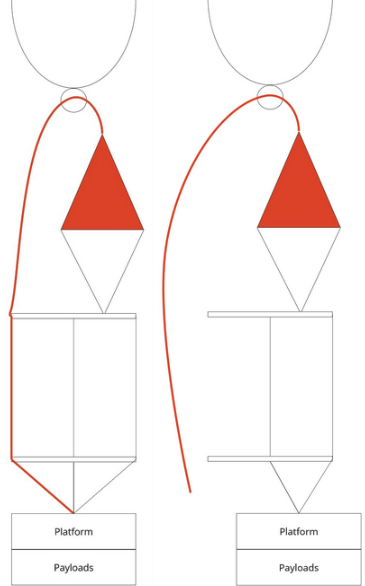
\includegraphics[width=0.8\linewidth]{rigging_cutter}
\end{minipage}
\captionof{figure}{Zestaw lotny z odcinaczem mechanicznym. Z prawej: schemat z misji z 26.05.2023 przed odcięciem i po odcięciu; czerwona linia -- linka odcinacza i zapas linki~\cite{pac2024}.}\label{fig:zestaw}
\end{sekcja}

\begin{sekcja}{Zestaw lotny w powietrzu}
\begin{minipage}[c]{0.4\linewidth}\centering
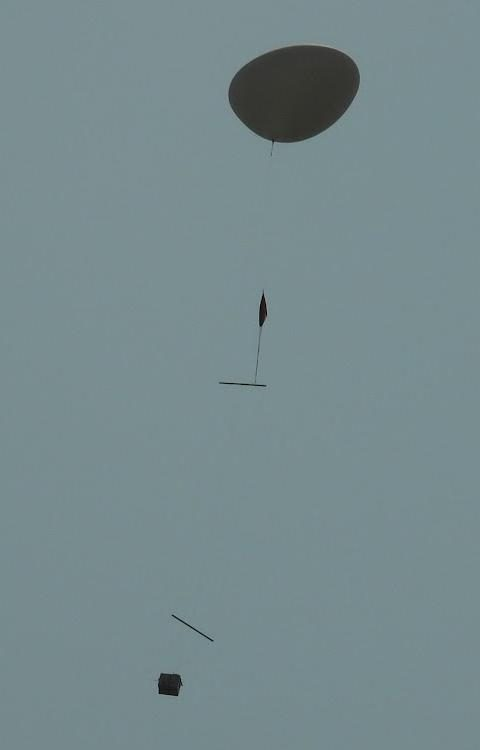
\includegraphics[width=\linewidth]{2023_zestaw_w_powietrzu_kadr}
\end{minipage}\hfill
\begin{minipage}[c]{0.55\linewidth}
Zestaw lotny Stardust NEXT krótko po starcie. Od góry widać:
\begin{enumerate}
  \item powłokę,
  \item spadochron (czerwony) na lince pod powłoką,
  \item poprzeczki z rurki na olinowaniu,
  \item zapas linki,
  \item gondolę.
\end{enumerate}
Linki są napięte, a elementy wiszą w jednej linii. Tak powinien wyglądać zestaw po prawidłowym starcie.
\end{minipage}
\captionof{figure}{Stardust NEXT w powietrzu (kadr ze zdjęcia z ziemi).}
\end{sekcja}

\begin{sekcja}{Powłoka}
\begin{itemize}
  \item Typ: lateksowa powłoka meteorologiczna (np. Hwoyee, Kaymont, Pawan). Dostawca w Polsce: \url{https://nearspace.pl/}.
  \item Wybierz rozmiar w kalkulatorze (rozdział~\ref{ch:planowanie}). Większa powłoka pęka wyżej, ale potrzebuje więcej gazu.
  \item Gaz nośny: hel. Wodór jest palny i wymaga dodatkowych środków bezpieczeństwa.
  \item Przechowuj powłokę w oryginalnym opakowaniu, w ciemnym i chłodnym miejscu.
  \item Dotykaj powłoki tylko w czystych rękawiczkach.
\end{itemize}
\end{sekcja}

\begin{sekcja}{Spadochron}
\begin{itemize}
  \item Dobierz spadochron do masy ładunku. Docelowa prędkość lądowania: około \SI{5}{m/s}.
  \item Spadochron wisi pod krętlikiem, nad gondolami. Jest stale otwarty -- nie ma mechanizmu wyrzutu.
  \item Kolor i średnicę spadochronu wpisz do zgłoszenia PAŻP.
\end{itemize}
\end{sekcja}

\begin{sekcja}{Olinowanie}
\textbf{Materiały:} taśma parciana, regulatory do taśmy (plastikowe albo metalowe), linka o średnicy około \SI{1}{mm} i wytrzymałości poniżej \SI{230}{N}, krętlik.

\textbf{Zasady:}
\begin{enumerate}
  \item Krętlik montuj bezpośrednio pod powłoką, na krótkiej pętli przywiązanej do szyjki. Krętlik zmniejsza skręcanie linek.
  \item Dodaj 10--15~m zapasu linki między spadochronem a gondolą. Zapas daje spadochronowi miejsce na otwarcie, gdy linki się skręcą.
  \item Gondole łącz taśmą z regulatorami. Regulatory pozwalają szybko wyrównać długości na stanowisku.
  \item Zabezpiecz każdy węzeł taśmą klejącą.
  \item Rozkładaj olinowanie na ziemi w linii, z wiatrem, bez pętli (rysunek~\ref{fig:pociag}).
\end{enumerate}

\foto[0.85\linewidth]{2023_zestaw_przed_startem}{Zestaw rozłożony przed startem: gondola na pierwszym planie, linka rozciągnięta w stronę stanowiska tankowania. Biała rurka pomaga rozłożyć linkę bez splątania.}\label{fig:pociag}
\end{sekcja}

\begin{sekcja}{Odcinacz mechaniczny -- zasada działania}
Odcinacz kończy lot na komendę albo automatycznie. Odcinacz oddziela gondole ze spadochronem od powłoki.

Odcinacz jest w gondoli platformy, nie pod balonem. Linka odcinacza biegnie od powłoki w dół do gondoli i jest zaczepiona o \textbf{zwalniacz serwomechaniczny} na pokrywie gondoli. Gdy serwo zwalnia linkę, gondole odłączają się od powłoki i opadają na spadochronie.

\textbf{Zalety:} cała elektronika jest w jednej gondoli. Odcinacz nie wymaga zasilania pod balonem.

\textbf{Wada:} obrót gondoli skręca linki. Skręcone linki mogą zablokować linkę odcinacza (misja z 26.05.2023).

\foto[0.55\linewidth]{2023_gondola_gora}{Pokrywa gondoli platformy: płyta montażowa (niebieska) ze zwalniaczem serwomechanicznym i zaczepioną linką, pasy z regulatorami, dwie anteny GPS.}
\end{sekcja}

\begin{sekcja}{Odcinacz mechaniczny -- wymagania}
\begin{itemize}
  \item Zwalniacz ładunku sterowany serwem (PWM, zasilanie 5--\SI{7.2}{V}, masa około \SI{76}{g}), np. zwalniacz zrzutu ładunku do dronów.
  \item Odcinacz działa na komendę z ziemi albo automatycznie: po czasie, po przekroczeniu wysokości, po wyjściu z dozwolonego obszaru, po długim locie poziomym (balon nie pękł).
  \item Komputer bezpieczeństwa (HABduino) steruje odcinaczem głównym. Komputer pokładowy (OBC) steruje \textbf{drugim, niezależnym odcinaczem innego typu}, np. z drutem oporowym (rozdział~\ref{ch:elektronika}).
  \item Testy: \SI{-40}{\degreeCelsius}, pełne obciążenie, skręcone linki (rozdział~\ref{ch:planowanie}).
  \item Na stanowisku sprawdź zwolnienie linki bez obciążenia, potem zaczep linkę i uzbrój odcinacz.
\end{itemize}

\renewcommand{\arraystretch}{1.3}
\small
\begin{tabularx}{\linewidth}{@{}P{32mm}P{38mm}L@{}}
\toprule
\textbf{Problem} & \textbf{Przyczyna} & \textbf{Środek zaradczy}\\\midrule
Linka odcinacza nie zwolniła się & Skręcone linki pod gondolą (brak krętlika na dole) & Zapas linki 10--15~m. Drugi krętlik nad gondolą. Prowadzenie linki odcinacza tak, aby skręt jej nie blokował.\\
Drut oporowy nie przeciął linki & Za krótki czas grzania & Testy w niskiej temperaturze i ciśnieniu. Dłuższy czas grzania. Bateria o większej wydajności prądowej.\\
\bottomrule
\end{tabularx}
\normalsize
\end{sekcja}

\begin{sekcja}{Gondola}
Gondola to pudełko styropianowe w rozmiarze typu eurobox (np. styrobox STX3-7, \SI{5}{l}). Pudełka są tanie, lekkie, izolują ciepło i chronią sprzęt przy lądowaniu. Mają standardowe wymiary, więc łatwo je łączyć ze sobą i z ładunkami zespołów badawczych.

\begin{center}\resizebox{0.9\linewidth}{!}{\rysGondola}\end{center}
\captionof{figure}{Przekrój gondoli: platforma (u góry) i ładunek badawczy (u dołu), spięte pasami.}\label{fig:gondola}
\end{sekcja}

\begin{sekcja}{Budowa gondoli platformy}
\begin{itemize}
  \item \textbf{Wkładka}: na dnie pudełka zamocuj płytę z lekkiego i wytrzymałego materiału (plexi, sklejka, włókno węglowe). Wszystkie elementy mocuj do wkładki: rzepem, śrubami, opaskami zaciskowymi. Uderzenie przy lądowaniu jest bardzo silne. Luźny element może zniszczyć resztę sprzętu, w tym karty pamięci -- a utrata danych to utrata całej misji.
  \item \textbf{Równowaga}: rozmieść elementy równomiernie. Środek masy musi leżeć w osi zawieszenia, aby gondola wisiała poziomo.
  \item \textbf{Płyta montażowa na pokrywie}: zwalniacz serwomechaniczny i mocowanie pasów.
  \item Gondola platformy zawiera tylko elektronikę platformy: tracker, OBC, odcinacz, lokalizatory, baterie.
  \item Anteny nadajników wyprowadź w dół. Antenę GPS umieść na górze, z widokiem na niebo, z dala od metalu.
  \item Opisz pudełko markerem: numer telefonu, „Projekt badawczy”, logo (rozdział~\ref{ch:prawo}).
\end{itemize}
\end{sekcja}

\begin{sekcja}{Gondola na zdjęciach}
\foto[0.8\linewidth]{2023_gondola_otwarta}{Gondola platformy otwarta: wkładka (czarna plexi) z elementami mocowanymi na rzep, śruby i opaski. Pokrywa z płytą montażową (niebieska), zwalniaczem i pasami.}
\dwafoto{2023_gondola_bok_anteny}{Anteny wyprowadzone w dół z boku gondoli.}
{2023_gondola_bok_termometr}{Platforma (u góry) i ładunek (u dołu) spięte pasami; czujnik temperatury na zewnątrz.}
\end{sekcja}

\begin{sekcja}{Anteny gondoli}
Antena typu dipol wymaga przeciwwagi. W powietrzu nie ma uziemienia -- przeciwwagą są przewody i elektronika w gondoli, co zmienia charakterystykę anteny.

Do rozważenia w kolejnych wersjach platformy:
\begin{itemize}
  \item metalowa płyta pod gondolą jako przeciwwaga i reflektor,
  \item antena ćwierćfalowa skierowana w dół, z luźnymi przewodami przeciwwagi (\emph{ground plane}),
  \item pomiar dopasowania anteny (SWR) w konfiguracji lotnej, w gondoli.
\end{itemize}
\end{sekcja}

\begin{sekcja}{Gondola ładunku badawczego}
\begin{itemize}
  \item Ładunek ma własne pudełko tego samego typu. Pudełka łączą się pasami.
  \item Ładunek ma własne zasilanie i własne oznakowanie.
  \item Ładunek przechodzi te same testy co platforma (rozdział~\ref{ch:planowanie}).
  \item Zespół badawczy podaje masę i częstotliwości radiowe (rozdział~\ref{ch:planowanie}).
\end{itemize}
\end{sekcja}

\chapter{Elektronika i łączność}\label{ch:elektronika}

\begin{sekcja}{Architektura}
Elektronika platformy jest w gondoli platformy. Zawiera:
\begin{itemize}
  \item \textbf{komputer bezpieczeństwa} (HABduino): GPS, telemetria, odcinacz główny,
  \item \textbf{komputer pokładowy} (OBC): zapis danych, zapasowe funkcje bezpieczeństwa, odcinacz zapasowy,
  \item \textbf{lokalizatory po lądowaniu}: SPOT Trace, dwa znaczniki Bluetooth (Apple i Google),
  \item baterie.
\end{itemize}

\begin{center}\resizebox{\linewidth}{!}{\rysTorRadiowy}\end{center}
\captionof{figure}{Tor radiowy: od gondoli przez stacje odbiorcze do map śledzenia.}\label{fig:tor-radiowy}
\end{sekcja}

\begin{sekcja}{Komputer bezpieczeństwa: HABduino}
HABduino to nakładka na Arduino do trackerów balonowych~\cite{habduino}. Nadaje telemetrię RTTY (moduł Radiometrix NTX2B, \SI{434}{MHz}) i APRS (\SI{144.8}{MHz}). Projekt nie jest już rozwijany. Zalecane oprogramowanie to FlexTrack~\cite{flextrack}: obsługuje HABduino~v4, RTTY i APRS, zawiera obsługę odcinacza. Opis budowy trackera: \cite{akerman}.

HABduino jest \textbf{głównym komputerem bezpieczeństwa}:
\begin{itemize}
  \item podaje pozycję (GPS) przez dwa niezależne łącza radiowe,
  \item steruje odcinaczem głównym (na komendę i automatycznie),
  \item działa niezależnie od OBC i od ładunku.
\end{itemize}
\end{sekcja}

\begin{sekcja}{Komputer pokładowy (OBC)}
OBC dodatkowo implementuje te same funkcje bezpieczeństwa, ale niezależnie od HABduino:
\begin{itemize}
  \item własny odbiornik GPS i własne kryteria zakończenia lotu,
  \item \textbf{niezależny odcinacz innego typu} (np. z drutem oporowym, gdy główny jest serwomechaniczny) -- jedna przyczyna awarii nie wyłącza obu,
  \item zapis danych z czujników na karcie SD, ze znacznikiem czasu,
  \item zapis stanu misji w pamięci nieulotnej: restart w locie nie zeruje misji.
\end{itemize}

\textbf{Wymagania:}
\begin{itemize}
  \item Wysokość bierz z GPS. Wzór na wysokość z ciśnienia jest niedokładny powyżej około \SI{10}{km}.
  \item Odrzucaj błędne odczyty czujników (kody błędów, wartości poza zakresem).
  \item Czujniki ciśnienia muszą mierzyć do około \SI{5}{hPa} (BME280 mierzy tylko do \SI{300}{hPa}).
  \item Dodaj diody statusu: zasilanie, GPS, karta SD, stan odcinacza.
\end{itemize}
Kod i dokumentacja OBC: \url{https://github.com/simle-stardust}.
\end{sekcja}

\begin{sekcja}{Konfiguracja trackera}
\begin{enumerate}
  \item Ustaw znak wywoławczy krótkofalowca (\emph{callsign}).
  \item Ustaw SSID APRS (zwyczajowo \texttt{-11} dla balonów).
  \item Ustaw identyfikator ładunku RTTY (\emph{payload ID}), taki sam jak w SondeHub.
  \item Ustaw moduł GPS w tryb \emph{airborne} (działa powyżej \SI{18}{km}; moduły u-blox do około \SI{50}{km}).
  \item Wgraj program. Zapisz wersję (numer commita albo wydania) w karcie misji.
\end{enumerate}

\begin{uwaga}Skonfiguruj tracker i serwisy śledzenia \textbf{najpóźniej 2 dni przed lotem}. Niektóre ustawienia (np. konfiguracja ładunku w SondeHub) potrzebują czasu, aby zadziałały. Dzień przed lotem zostaw na weryfikację, logistykę i obserwację pogody.\end{uwaga}
\end{sekcja}

\begin{sekcja}{Anteny i test zasięgu}
\begin{itemize}
  \item Antenę nadajnika montuj pod gondolą, skierowaną w dół.
  \item Antenę GPS montuj na górze gondoli, z widokiem na niebo, z dala od baterii i metalu.
  \item Po montażu sprawdź złącza i przewody anten.
\end{itemize}

\begin{uwaga}Z bliska odbiornik odbierze sygnał nawet bez anteny -- wystarczy promieniowanie z płytki i przewodów. Test obok stołu niczego nie dowodzi. Sprawdź odbiór z odległości \textbf{co najmniej \SI{100}{m}}, z anteną w konfiguracji lotnej (w zamkniętej gondoli).\end{uwaga}
\end{sekcja}

\begin{sekcja}{Lokalizatory po lądowaniu}
Przy ziemi sygnał z trackera zanika: zasłaniają go drzewa, budynki i ukształtowanie terenu. Lokalizatory pomagają znaleźć gondolę po lądowaniu.

\begin{itemize}
  \item \textbf{SPOT Trace} -- lokalizator satelitarny. Działa tylko do około \SI{6500}{m}, więc służy tylko po lądowaniu. Wymaga aktywnej subskrypcji. Ustaw interwał raportów (np. 5 minut). Antena do góry.
  \item \textbf{Znaczniki Bluetooth: Apple AirTag i znacznik sieci Google (Find Hub)} -- najlepiej dwa niezależne. Smartfony w pobliżu przekazują pozycję znacznika. Gdy ktoś znajdzie gondolę przed zespołem i podejdzie ze smartfonem, zespół zobaczy nową pozycję.
  \item Zapasowo: smartfon z funkcją „Znajdź moje urządzenie” -- w 2020 roku pomógł znaleźć ładunek~\cite{raport2020}.
\end{itemize}
\end{sekcja}

\begin{sekcja}{Zasilanie}
\begin{itemize}
  \item Używaj baterii litowych, np. Energizer Ultimate Lithium (Energizer Extreme). Działają w niskiej temperaturze i są lekkie.
  \item Włóż nowe baterie przed każdym lotem.
  \item Licz budżet energii: pobór każdego urządzenia $\times$ czas pracy $\times$ zapas. Uwzględnij prąd rozruchowy serw i grzałek.
  \item Czas pracy: co najmniej dwa razy dłuższy niż planowany lot plus czas poszukiwań.
\end{itemize}
\end{sekcja}

\begin{sekcja}{Termika: mróz i próżnia}
W stratosferze powietrze ma do \SI{-60}{\degreeCelsius}, ale jest bardzo rzadkie. Prawie nie ma konwekcji, więc elektronika \textbf{nie oddaje ciepła} do powietrza. Słońce dodatkowo nagrzewa gondolę. W misji z lipca 2020 roku elektronika w izolowanej gondoli przekroczyła \SI{50}{\degreeCelsius}~\cite{praca2022}.

\textbf{Zasady projektowe:}
\begin{itemize}
  \item projektuj elektronikę o wysokiej sprawności -- mniej strat to mniej ciepła,
  \item dodaj duży zapas pojemności cieplnej (masa, która akumuluje ciepło, np. baterie, metalowa płyta),
  \item odprowadzaj ciepło przez przewodzenie do obudowy, nie przez powietrze,
  \item nie dodawaj izolacji ani grzałek bez bilansu cieplnego dla startu (zimno) i dla stratosfery (brak chłodzenia).
\end{itemize}

\begin{wskazowka}Do testów w niskiej temperaturze zapytaj biologów na Wydziale Chemicznym o zamrażarkę laboratoryjną (\SI{-80}{\degreeCelsius}).\end{wskazowka}
\end{sekcja}

\chapter{Oprogramowanie}\label{ch:oprogramowanie}

\begin{sekcja}{Narzędzia}
\renewcommand{\arraystretch}{1.3}
\begin{tabularx}{\linewidth}{@{}P{34mm}LP{50mm}@{}}
\toprule
\textbf{Narzędzie} & \textbf{Zastosowanie} & \textbf{Adres}\\\midrule
SondeHub Burst Calculator & Ilość gazu, siła nośna, wysokość pęknięcia & \www{sondehub.org/calc}\\
SondeHub Predictor & Predykcja trajektorii i miejsca lądowania & \www{predict.sondehub.org}\\
SondeHub Amateur & Mapa śledzenia (APRS, RTTY, LoRa, Horus) & \www{amateur.sondehub.org}\\
aprs.fi & Mapa śledzenia APRS & \www{aprs.fi}\\
PureTrack & Mapa śledzenia & \www{puretrack.io}\\
SPOT & Lokalizator satelitarny & \www{www.findmespot.com}\\
Find My / Find Hub & Znaczniki Bluetooth & aplikacje Apple i Google\\
\bottomrule
\end{tabularx}
\end{sekcja}

\begin{sekcja}{Konfiguracja przed misją}
Wykonaj najpóźniej \textbf{2 dni przed lotem} (formularz F7):
\begin{enumerate}
  \item Wejdź na \www{amateur.sondehub.org} i skonfiguruj dokument ładunku (\emph{payload}) dla RTTY. Bez tego SondeHub nie zdekoduje telemetrii.
  \item Włącz tracker na zewnątrz. Wejdź na \www{aprs.fi} i sprawdź, czy pozycja znaku z SSID pojawia się na mapie.
  \item Wejdź na SondeHub Amateur i sprawdź, czy pakiety RTTY pojawiają się na mapie.
  \item Aktywuj subskrypcję SPOT (plan Flex -- na jeden miesiąc). Wejdź na stronę SPOT i sprawdź pozycję urządzenia.
  \item Dodaj znaczniki Bluetooth do kont Apple i Google zespołu. Sprawdź ich pozycję w aplikacjach.
  \item Udostępnij linki do śledzenia całemu zespołowi.
\end{enumerate}
\end{sekcja}

\begin{sekcja}{Wersja kodu lotnego}
Kod lotny (HABduino, OBC, ładunek) i dokumentacja tworzą jedną całość:
\begin{itemize}
  \item w dokumentacji misji (karta misji F0, raport) zapisz wersję kodu lotnego: numer wydania (\emph{release}) albo commita,
  \item do wydania kodu lotnego dołącz końcową wersję dokumentacji (np. PDF tego podręcznika i raport z misji),
  \item nie zmieniaj kodu po przeglądzie gotowości. Każda zmiana po przeglądzie wymaga ponownych testów.
\end{itemize}

Gdy po przeglądzie znajdziesz błąd:
\begin{itemize}
  \item \textbf{błąd krytyczny} (zagraża bezpieczeństwu albo celowi misji): popraw kod, powtórz testy i przegląd gotowości albo przełóż lot,
  \item \textbf{błąd niekrytyczny}: nie zmieniaj kodu. Bardziej wartościowe jest zrozumienie, kiedy błąd występuje, i opracowanie procedury obejścia poza kodem -- np. zmiana sekwencji uruchomienia albo kolejności telekomend. Zapisz obejście w formularzach dnia startu i w raporcie.
\end{itemize}
\end{sekcja}

\begin{sekcja}{Konfiguracja komputerów bez przeprogramowania}\label{sec:konfiguracja}
Kod lotny nie zmienia się po przeglądzie gotowości, ale parametry misji tak: wysokość i czas zadziałania odcinacza, granice dozwolonego obszaru, parametry lotu, godzina startu. Zespół musi wpisywać te wartości \textbf{bez przeprogramowania} komputera.

Zespół tworzy własną procedurę obsługi każdego komputera (HABduino, OBC, ładunek). Procedura określa, jak wpisać wartości i kto to robi. Możliwe sposoby:
\begin{itemize}
  \item kabel i komendy, które zapisują konfigurację w pamięci trwałej komputera,
  \item telekomendy -- tylko gdy komputer ma odbiornik,
  \item karta SD z plikiem konfiguracyjnym, wymieniana przed startem.
\end{itemize}

\textbf{Zasady:}
\begin{enumerate}
  \item Przygotuj konfigurację dla \textbf{każdego scenariusza misji} (np. miejsce startu zasadnicze i zapasowe, opóźniony start). Nadaj każdej konfiguracji nazwę scenariusza i zapisz ją w dokumentacji misji.
  \item Przetestuj każdą konfigurację przed lotem, tą samą drogą, którą wpiszesz ją w dniu startu.
  \item Po wpisaniu odczytaj konfigurację z komputera i porównaj z zapisaną. Nie sprawdzaj pliku na laptopie -- sprawdź to, co jest w komputerze.
  \item Ustawień, które zmieniają się w locie (z wysokością albo czasem), test na ziemi nie sprawdzi. Przeczytaj je w konfiguracji (sekcja~\ref{sec:konfiguracja-trackera}).
  \item Zapisz w formularzach dnia startu, którą konfigurację wpisano do którego komputera. Zachowaj pliki konfiguracyjne z lotu do późniejszej weryfikacji.
\end{enumerate}
\end{sekcja}

\chapter{Instrukcje montażu}\label{ch:montaz}

Montuj zestaw według tej kolejności. Każdy podzespół ma osobę odpowiedzialną (formularz F1). Po każdym kroku zaznacz go w formularzu.

\begin{sekcja}{Wkładka gondoli}
Wkładka to płyta montażowa na dnie pudełka. Do wkładki mocujesz całą elektronikę.
\begin{enumerate}
  \item Wytnij płytę z lekkiego i wytrzymałego materiału: plexi, sklejka albo włókno węglowe. Wymiar: wewnętrzne dno pudełka.
  \item Rozplanuj elementy tak, aby środek masy był na środku płyty.
  \item Wywierć otwory na śruby i opaski zaciskowe. Przyklej rzepy pod lekkie elementy.
  \item Zamocuj płytę w pudełku (klej do styropianu albo śruby z podkładkami przez dno).
\end{enumerate}

\begin{uwaga}Uderzenie przy lądowaniu jest bardzo silne. Każdy element musi być przymocowany do wkładki. Karta pamięci musi być zabezpieczona przed wypadnięciem (taśma na gnieździe). Utrata danych to utrata całej misji.\end{uwaga}
\end{sekcja}

\begin{sekcja}{Gondola platformy}
\begin{enumerate}
  \item Zważ puste pudełko.
  \item Zamocuj do wkładki: HABduino, OBC, baterie, SPOT, znaczniki Bluetooth.
  \item Poprowadź anteny nadajników przez ścianę albo dno pudełka. Anteny skierowane w dół.
  \item Zamocuj antenę GPS pod pokrywą albo na pokrywie, z dala od baterii i metalu.
  \item Zamocuj płytę montażową na pokrywie. Zamocuj zwalniacz serwomechaniczny. Poprowadź przewód serwa do środka.
  \item Podłącz baterie. Sprawdź diody statusu.
  \item Sprawdź odbiór telemetrii z odległości co najmniej \SI{100}{m}.
  \item Sprawdź zwolnienie odcinacza na komendę.
  \item Sprawdź równowagę: zawieś gondolę na linkach. Gondola wisi poziomo.
  \item Wyłącz zasilanie. Zważ gondolę. Wpisz masę do budżetu masy.
\end{enumerate}
\end{sekcja}

\begin{sekcja}{Olinowanie}
\begin{enumerate}
  \item Przytnij taśmy na długość. Zamontuj regulatory.
  \item Połącz gondolę ładunku z gondolą platformy taśmą (dookoła obu pudełek, na krzyż).
  \item Przygotuj krótką pętlę do szyjki powłoki z krętlikiem.
  \item Przywiąż spadochron pod krętlikiem.
  \item Przygotuj zapas linki 10--15~m między spadochronem a gondolą. Zwiń zapas na kartonie albo rurce, aby się nie splątał.
  \item Przygotuj linkę odcinacza: od krętlika do zwalniacza w gondoli.
  \item Zważ olinowanie ze spadochronem. Wpisz masę do budżetu masy.
\end{enumerate}
\end{sekcja}

\begin{sekcja}{Kontrola w warsztacie}
\begin{itemize}
  \item[\kratka] Łączna masa ładunku poniżej \SI{4}{kg}.
  \item[\kratka] Każdy pakiet poniżej \SI{2}{kg}.
  \item[\kratka] Opis markerem na każdym pakiecie: telefon, „Projekt badawczy”, logo.
  \item[\kratka] Wszystkie testy z formularza F5 zaliczone.
  \item[\kratka] Wszystko spakowane według wykazu materiałów.
\end{itemize}
\end{sekcja}

\begin{sekcja}{Na stanowisku startowym}
\begin{enumerate}
  \item Rozłóż podłoże: plandeka, koc, folia dolna. Dociśnij rogi skrzynkami.
  \item Rozłóż zestaw lotny w linii, z wiatrem: krętlik, spadochron, zapas linki, gondole.
  \item Włącz elektronikę platformy i ładunku. Sprawdź pozycję GPS i odbiór telemetrii na mapach.
  \item Zatankuj powłokę (rozdział~\ref{ch:naziemny}).
  \item Zamknij szyjkę. Przywiąż pętlę z krętlikiem.
  \item Zaczep linkę odcinacza o zwalniacz. Uzbrój odcinacz.
  \item Sprawdź węzły. Zabezpiecz je taśmą.
  \item Zamknij gondole. Owiń je taśmą. Napnij pasy.
  \item Wykonaj formularz F11 „Start”.
\end{enumerate}
\end{sekcja}

\begin{sekcja}{Start}
\begin{enumerate}
  \item Pomocnicy trzymają powłokę folią górną. Jedna osoba trzyma gondolę.
  \item Kierownik startu sprawdza niebo (samoloty) i odlicza.
  \item Na komendę pomocnicy zdejmują folię i puszczają powłokę. Osoba z gondolą idzie pod wiatr, aż linki się naprężą.
  \item Osoba z gondolą puszcza gondolę, gdy gondola jest pod balonem. Nie rzucaj gondoli.
  \item Zapisz czas startu.
\end{enumerate}

\dwafoto{2020_start_torun}{Start: powłoka unosi linkę, zespół trzyma gondolę (20.07.2020).}
{2023_zestaw_przed_startem}{Zestaw rozłożony z wiatrem przed startem (26.05.2023).}
\end{sekcja}

\chapter{Wykaz materiałów i narzędzi}\label{ch:materialy}

Ceny i dostawcy się zmieniają. Przed zakupem sprawdź dostępność. Pozycje jednorazowe kupuj na każdą misję. Pozycje wielokrotne sprawdź w szafce co najmniej 4 tygodnie przed lotem. Kolumna „OK” służy do kontroli przy pakowaniu.

\begin{landscape}
\section{Segment lotny}
\renewcommand{\arraystretch}{1.35}
\small
\begin{longtable}{@{}C{8mm}P{58mm}P{22mm}P{20mm}P{58mm}P{44mm}@{}}
\toprule
\textbf{OK} & \textbf{Pozycja} & \textbf{Ilość} & \textbf{Typ} & \textbf{Źródło / przykład} & \textbf{Uwagi}\\\midrule\endhead
\bottomrule\endfoot
\kratka & Powłoka lateksowa & 1 & jednorazowa & nearspace.pl & Rozmiar z kalkulatora.\\
\kratka & Spadochron & 1 & wielokrotna & nearspace.pl & Dobierz do masy ładunku.\\
\kratka & Krętlik & 1--2 & wielokrotna & sklep wędkarski albo żeglarski & \\
\kratka & Taśma parciana & kilka m & wielokrotna & pasmanteria & \\
\kratka & Regulatory do taśmy & kilka & wielokrotna & pasmanteria, ustefana.pl & Plastikowe albo metalowe.\\
\kratka & Linka ok. 1 mm (zrywalność $<$ \SI{230}{N}) & ok. 30 m & jednorazowa & & Z zapasem 10--15 m.\\
\kratka & Zwalniacz serwomechaniczny & 1 & wielokrotna & sklepy z akcesoriami do dronów & PWM, 5--\SI{7.2}{V}.\\
\kratka & Odcinacz zapasowy (drut oporowy) & 1 & wielokrotna & własna konstrukcja & Sterowany przez OBC.\\
\kratka & Pudełko styropianowe typu eurobox (np. STX3-7, \SI{5}{l}) & 1 + 1 na ładunek & wielokrotna & allegro.pl (styrobox) & \\
\kratka & Wkładka (plexi / sklejka / włókno węglowe) & 1 & wielokrotna & & Na dno gondoli.\\
\kratka & Tracker HABduino z FlexTrack & 1 & wielokrotna & github.com/HABduino & \\
\kratka & Komputer pokładowy (OBC) & 1 & wielokrotna & github.com/simle-stardust & \\
\kratka & Lokalizator SPOT Trace & 1 & wielokrotna & findmespot.com & Wymaga subskrypcji.\\
\kratka & Znaczniki Bluetooth (Apple AirTag, znacznik Google Find Hub) & 2 & wielokrotna & & Dwa niezależne.\\
\kratka & Baterie litowe (Energizer Ultimate Lithium) & komplet & jednorazowa & & Nowe na każdy lot.\\
\kratka & Marker permanentny, naklejki z logo & 1 & wielokrotna & & Opis gondoli.\\
\end{longtable}

\section{Segment naziemny}
\begin{longtable}{@{}C{8mm}P{58mm}P{22mm}P{20mm}P{58mm}P{44mm}@{}}
\toprule
\textbf{OK} & \textbf{Pozycja} & \textbf{Ilość} & \textbf{Typ} & \textbf{Źródło / przykład} & \textbf{Uwagi}\\\midrule\endhead
\bottomrule\endfoot
\kratka & Hel (butla \SI{50}{l}, \SI{200}{bar}) & wg kalkulatora + 30\,\% & jednorazowa & dostawca gazów technicznych & Zamów z wyprzedzeniem.\\
\kratka & Reduktor z manometrem i wąż & 1 & wielokrotna & & Sprawdź gwint butli.\\
\kratka & Rura do tankowania (z zaworem zwrotnym) & 1 & wielokrotna & nearspace.pl & \\
\kratka & Obciążnik (butelka na wodę) i waga & 1 & wielokrotna & & Masa = siła nośna szyjki.\\
\kratka & Plandeka & 1 & wielokrotna & market budowlany & Warstwa dolna.\\
\kratka & Koc (gruby) & 1--2 & wielokrotna & & \\
\kratka & Folia malarska cienka i grubsza & po 1 & jednorazowa & market budowlany & \\
\kratka & Skrzynki transportowe & 4 & wielokrotna & & Dociskają rogi.\\
\kratka & Rękawiczki (bawełniane, nitrylowe) & opakowanie & jednorazowa & & Dla wszystkich przy powłoce.\\
\kratka & Taśma klejąca, sznurek, opaski zaciskowe & & jednorazowa & & Zamknięcie szyjki.\\
\kratka & Radiotelefon APRS (np. Yaesu FT5DE) & 1 & wielokrotna & & Stacja mobilna.\\
\kratka & Antena samochodowa VHF/UHF na magnes (np. Nagoya UT-72) & 1 & wielokrotna & & \\
\kratka & RTL-SDR + LNA + filtry + laptop & 1 & wielokrotna & & Alternatywa / zapas.\\
\end{longtable}

\section{Narzędzia i wyposażenie}
\begin{longtable}{@{}C{8mm}P{58mm}P{22mm}P{20mm}P{58mm}P{44mm}@{}}
\toprule
\textbf{OK} & \textbf{Pozycja} & \textbf{Ilość} & \textbf{Typ} & \textbf{Źródło / przykład} & \textbf{Uwagi}\\\midrule\endhead
\bottomrule\endfoot
\kratka & Klucz nastawny, klucze calowe & 1 kpl. & wielokrotna & & Do reduktora.\\
\kratka & Nożyczki, nóż, śrubokręty & 1 kpl. & wielokrotna & & \\
\kratka & Wydrukowane formularze i ten manual & 1 kpl. & jednorazowa & dodatek A & Długopisy, podkładka.\\
\kratka & Laptop, telefony z internetem & & wielokrotna & & \\
\kratka & Powerbank, ładowarka samochodowa, rozgałęźnik & & wielokrotna & & \\
\kratka & Aparat fotograficzny & 1 & wielokrotna & & Rola: fotograf.\\
\kratka & Samochód pościgowy (najlepiej dwa) & 1--2 & & & \\
\kratka & Apteczka, woda, prowiant, odzież & & & & \\
\end{longtable}
\end{landscape}

\chapter{Prowadzenie projektu i dokumentacja}\label{ch:projekt}

Ten rozdział opisuje, jak prowadzić projekt misji i dokumentację eksperymentu. Praktyki pochodzą z programu REXUS/BEXUS (ESA, DLR, SNSA), w którym zespół Stardust uczestniczył~\cite{praca2022,sed}. Program prowadzi zespoły studenckie przez pełny cykl misji kosmicznej. Uproszczona wersja tych praktyk działa dobrze w misjach własnych.

\begin{sekcja}{Cykl projektu}
Podziel projekt na etapy. Na końcu każdego etapu zrób przegląd: zespół przedstawia stan projektu osobom spoza zespołu (absolwentom projektu, opiekunowi koła, zespołowi badawczemu). Przegląd kończy się listą działań z osobami odpowiedzialnymi i terminami.

\renewcommand{\arraystretch}{1.3}
\small
\begin{tabularx}{\linewidth}{@{}P{30mm}LL@{}}
\toprule
\textbf{Etap} & \textbf{Pytanie przeglądu} & \textbf{Wynik}\\\midrule
Koncepcja & Co chcemy zbadać i dlaczego? Czy to jest możliwe? & Cel, wymagania, wstępny budżet masy.\\
Projekt wstępny (PDR) & Czy koncepcja spełnia wymagania? & Schemat systemu, wybór komponentów, plan testów.\\
Projekt krytyczny (CDR) & Czy projekt jest gotowy do budowy? & Kompletny projekt, budżety, rejestr ryzyk.\\
Integracja i testy & Czy zbudowany sprzęt działa? & Wyniki testów (F5), poprawki.\\
Gotowość do lotu (FRR) & Czy możemy bezpiecznie polecieć? & Decyzja „leci / nie leci” (F6).\\
Po misji & Co działało? Co poprawić? & Raport, wnioski (F14).\\
\bottomrule
\end{tabularx}
\normalsize

Dla prostej misji szkoleniowej wystarczą dwa przeglądy: przed budową (CDR) i przed lotem (FRR).
\end{sekcja}

\begin{sekcja}{Dokumentacja eksperymentu}
Każdy ładunek i każda zmiana platformy ma dokument eksperymentu. Wzór: dokument SED (\emph{Student Experiment Documentation}) z programu REXUS/BEXUS. Przykład: dokument SED zespołu Stardust~\cite{sed}. Opis platformy BEXUS i wymagań wobec eksperymentów: BEXUS User Manual~\cite{bexusmanual}. Szablony przeglądów PDR, CDR i FRR dla studenckich ładunków balonowych udostępnia kurs LaACES~\cite{laaces}.

Minimalna struktura dokumentu eksperymentu:
\begin{enumerate}
  \item \textbf{Wprowadzenie} -- cel naukowy albo techniczny, zespół i role.
  \item \textbf{Wymagania} -- co eksperyment musi robić, jakie ma ograniczenia (masa, wymiary, zasilanie, temperatura).
  \item \textbf{Projekt} -- mechanika, elektronika, oprogramowanie (np. maszyna stanów).
  \item \textbf{Budżety} -- masa, energia, dane.
  \item \textbf{Rejestr ryzyk} -- co może się nie udać, prawdopodobieństwo, skutek, środek zaradczy.
  \item \textbf{Plan testów i wyniki} -- każde wymaganie ma test, który je weryfikuje.
  \item \textbf{Procedury} -- montaż, przygotowanie na stanowisku, formularze.
  \item \textbf{Wyniki i wnioski} -- po misji.
\end{enumerate}

Pisz dokument od początku projektu, nie po misji. Numeruj wersje. Zapisuj, co się zmieniło.
\end{sekcja}

\begin{sekcja}{Dokumentacja i kod}
Dokumentacja może być w repozytorium kodu albo w osobnym pliku. Ważne są dwa powiązania:
\begin{itemize}
  \item \textbf{dokumentacja w wydaniu kodu}: do wydania (\emph{release}) kodu lotnego dołącz końcową wersję dokumentacji i raport z misji,
  \item \textbf{wersja kodu w dokumentacji}: w karcie misji i w raporcie zapisz numer wydania albo commita kodu, który poleciał.
\end{itemize}
Ten podręcznik powstaje automatycznie z plików \LaTeX{} w repozytorium \www{github.com/simle-stardust/Manual}. Każde wydanie (tag \texttt{v*}) ma dołączony PDF.
\end{sekcja}

\begin{sekcja}{Budżety}
\textbf{Budżet masy:} tabela wszystkich elementów z masą zmierzoną. Zapas co najmniej \SI{10}{\percent}.

\textbf{Budżet energii:} dla każdego urządzenia: napięcie, prąd w pracy, prąd szczytowy, czas pracy. Suma energii $\times$ zapas $\leq$ pojemność baterii w niskiej temperaturze.

\textbf{Budżet danych:} dane na sekundę $\times$ czas lotu $\leq$ pojemność pamięci. Przepustowość łącza radiowego $\geq$ dane telemetrii.

\textbf{Budżet finansowy:} koszty jednorazowe (powłoka, hel, materiały, baterie, subskrypcje), koszty sprzętu wielokrotnego, transport, ubezpieczenie, zapas na powtórkę lotu. Budżet finansowy jest podstawą wniosku o dofinansowanie i oferty dla klienta (np. zespołu badawczego albo firmy, której ładunek leci). Zapisuj rzeczywiste koszty każdej misji -- następny budżet będzie dokładniejszy.
\end{sekcja}

\begin{sekcja}{Rejestr ryzyk}
\renewcommand{\arraystretch}{1.3}
\small
\begin{tabularx}{\linewidth}{@{}P{40mm}P{40mm}L@{}}
\toprule
\textbf{Ryzyko} & \textbf{Skutek} & \textbf{Środek zaradczy}\\\midrule
Odcinacz nie działa & Długi lot, lądowanie daleko & Testy w warunkach lotu, zapas linki, drugi odcinacz innego typu\\
Brak telemetrii & Utrata ładunku & Dwa systemy śledzenia, SPOT, znaczniki Bluetooth\\
Za mało gazu & Opóźniony start & Zapas gazu, pomiar siły nośnej\\
Rozładowana bateria & Brak danych i lokalizacji & Budżet energii, test w zimnie, nowe baterie\\
Lądowanie w wodzie lub za granicą & Utrata ładunku, incydent & Predykcja, kryteria braku startu, odcinacz\\
Restart OBC w locie & Utrata stanu misji & Stan w pamięci nieulotnej\\
Uszkodzenie przy lądowaniu & Utrata danych & Wkładka, mocowanie kart pamięci\\
\bottomrule
\end{tabularx}
\normalsize
\end{sekcja}

\begin{sekcja}{Nazwa, kryptonim i patch misji}\label{sec:patch}
Nadaj każdej misji nazwę i kryptonim, na przykład Antares (2018) albo Stormdust (2023). Używaj ich w dokumentach, nazwach plików, formularzach i w mediach -- wtedy misje w archiwum się nie mylą. Zaprojektuj też patch misji: naszywkę z nazwą, rokiem i symbolem celu misji (przykład: patch z 2023 roku na okładce). Patch łączy zespół, oznacza zdjęcia, prezentacje i koszulki oraz jest gotową grafiką do wpisów i podziękowań dla sponsorów. Zapisz nazwę, kryptonim i plik patcha w karcie misji (formularz F0).
\end{sekcja}

\begin{sekcja}{Zdjęcia i dokumentacja wizualna}
Zdjęcia to ważna część procedur. Służą do:
\begin{itemize}
  \item dokumentacji projektu -- jak sprzęt wyglądał w dniu startu,
  \item analizy po locie -- zdjęcia pokazują, co poszło nie tak (np. ułożenie linek, mocowanie anteny),
  \item promocji -- zdjęcia przyciągają sponsorów i nowych członków.
\end{itemize}

Wydziel osobną rolę: \textbf{fotograf / dokumentalista} (formularz F1). Fotograf nie ma innych zadań przy starcie. Fotograf fotografuje:
\begin{itemize}
  \item każdą gondolę otwartą i zamkniętą, przed zamknięciem,
  \item stanowisko, tankowanie, zamknięcie szyjki, zestaw przed startem,
  \item tankowanie i start -- w całości filmem. Przy anomalii film pozwala ustalić jej przyczynę~\cite[rozdz.~11]{nasahb},
  \item miejsce lądowania przed dotknięciem sprzętu.
\end{itemize}
\end{sekcja}

\begin{sekcja}{Raport z misji}
Napisz raport w ciągu tygodnia po misji. Wzór: raport z misji testowej 2020~\cite{raport2020}.
\begin{enumerate}
  \item Zestaw lotny: elementy, masy, wersje kodu.
  \item Oś czasu: NOTAM, start, pęknięcie albo odcięcie, lądowanie, odzyskanie.
  \item Dane z lotu: trasa, profil wysokości, czujniki (pliki w załączniku).
  \item Problemy: co nie działało i dlaczego.
  \item Wnioski: co zmienić w następnej misji.
  \item Plan zmian: co, kto, do kiedy~\cite[rozdz.~11]{nasahb}.
\end{enumerate}
Dopisz wnioski do rozdziału~\ref{ch:historia}.
\end{sekcja}

\begin{sekcja}{Przekazywanie wiedzy}
Zespoły studenckie zmieniają się co kilka lat. Wiedza ginie, gdy jest tylko w głowach.
\begin{itemize}
  \item Każda nowa grupa zaczyna od lotu szkoleniowego z prostym ładunkiem.
  \item Doświadczona osoba prowadzi pierwszą misję. Następną misję nowy zespół prowadzi samodzielnie.
  \item Każdy podzespół ma osobę odpowiedzialną i opisaną procedurę.
  \item Po każdej misji aktualizuj tę dokumentację.
  \item Publikuj wyniki (konferencje, artykuły, blog). Publikacje zostają po zespole.
\end{itemize}
\end{sekcja}

\begin{sekcja}{Dalsza lektura}
\begin{itemize}
  \item \textbf{NASA Scientific Ballooning Handbook} (wydanie na 50-lecie, 2025) -- kompendium wiedzy o balonach naukowych: teoria lotu, gazy nośne, operacje, spadochrony, łączność. Na początek przeczytaj rozdział~2 o balonach w edukacji (programy studenckie, wnioski zespołów BOREALIS i NEBP)~\cite{nasahb}.
  \item \textbf{Projekt Loon} (X, the moonshot factory) -- doświadczenia z tysięcy lotów balonów stratosferycznych: konstrukcja powłok, nawigacja z wiatrem, operacje. Kolekcja materiałów i podsumowanie „The Loon Library”~\cite{loon}.
  \item \textbf{BEXUS User Manual} -- opis platformy BEXUS i wymagań wobec eksperymentów~\cite{bexusmanual}.
  \item \textbf{Kursy balonowe dla studentów}: LaACES (elektronika, programowanie, zarządzanie projektem, szablony dokumentów)~\cite{laaces} oraz kursy projektu NEBP (planowanie misji i logistyka startu)~\cite{nebp}.
  \item \textbf{Akademia Stratosferycznie} -- bezpłatne kursy o misjach stratosferycznych po polsku~\cite{akademia}.
  \item Artykuły zespołu Stardust z konferencji IAC i ESA PAC~\cite{iac2023,pac2024}.
\end{itemize}
\end{sekcja}


\appendix
\chapter{Formularze}\label{dod:formularze}

\begin{blok}
Wydrukuj ten dodatek osobno dla każdej misji (jednostronnie). Wypełniaj formularze długopisem. Każdy formularz ma:
\begin{itemize}
  \item nagłówek z danymi misji i osobą wypełniającą,
  \item kroki w formie poleceń: \emph{wejdź na \dots{} i sprawdź \dots{}},
  \item pole „Wartość / uwagi” na odczyty, numery i nazwiska,
  \item miejsce na komentarze i podpisy.
\end{itemize}
Gdy krok jest niewykonalny, nie zaznaczaj go -- opisz odstępstwo w komentarzach. Kierownik misji decyduje, czy kontynuować.

Po misji zeskanuj wszystkie formularze i przechowuj skany w wewnętrznej dokumentacji koła. Wypełnione formularze zawierają dane osobowe (nazwiska, telefony) -- nie publikuj ich. Do publicznego raportu przenieś tylko dane techniczne i wnioski.

\medskip
\renewcommand{\arraystretch}{1.25}
\begin{tabularx}{\linewidth}{@{}P{12mm}LP{38mm}@{}}
\toprule
\textbf{Kod} & \textbf{Formularz} & \textbf{Kiedy}\\\midrule
F0 & Karta misji & cały projekt\\
F1 & Role w zespole i macierz odpowiedzialności & T$-$16 tyg.\\
F2 & Planowanie misji & T$-$16 do T$-$4 tyg.\\
F3 & Formalności & T$-$4 do T$-$2 tyg.\\
F4 & Dziennik predykcji & od T$-$7 dni\\
F5 & Raport z testów & przed FRR\\
F6 & Przegląd gotowości do startu (FRR) & T$-$7 do T$-$3 dni\\
F7 & Konfiguracja trackera i serwisów & T$-$2 dni\\
F8 & Weryfikacja i logistyka & T$-$1 dzień\\
F9 & Stanowisko startowe & T0\\
F10 & Tankowanie & T0\\
F11 & Start & T0\\
F12 & Lot i pościg (dziennik) & T0\\
F13 & Odzyskanie & T0\\
F14 & Po misji & do T+7 dni\\
\bottomrule
\end{tabularx}
\end{blok}

% ===========================================================================
\formularz[kierownik misji]{F0}{Karta misji (1/2)}{cały projekt}
\renewcommand{\arraystretch}{1.0}
\small
\begin{tabularx}{\linewidth}{@{}|L|L|@{}}\hline
\multicolumn{2}{|l|}{\cellcolor{sdlight}\rule{0pt}{4mm}\textbf{Misja}}\\\hline
\etykieta{Nazwa misji} & \etykieta{Kierownik misji (telefon)}\\\hline
\multicolumn{2}{|p{\dimexpr\linewidth-2\tabcolsep\relax}|}{\etykieta[40mm]{Cel misji (mission statement): co chcemy osiągnąć, po czym poznamy sukces}}\\\hline
\multicolumn{2}{|p{\dimexpr\linewidth-2\tabcolsep\relax}|}{\etykieta[18mm]{Ładunki badawcze (nazwa, zespół, opiekun)}}\\\hline
\multicolumn{2}{|l|}{\cellcolor{sdlight}\rule{0pt}{4mm}\textbf{Terminy i miejsca (zgodne ze zgłoszeniem PAŻP)}}\\\hline
\etykieta[11mm]{Scenariusz A: miejsce, współrzędne} & \etykieta[11mm]{Scenariusz A: data, godz. (UTC), termin zapasowy}\\\hline
\etykieta[11mm]{Scenariusz B: miejsce, współrzędne} & \etykieta[11mm]{Scenariusz B: data, godz. (UTC), termin zapasowy}\\\hline
\etykieta{Numery zgłoszeń PAŻP} & \etykieta{NOTAM (numer, sprawdzony w AIS: data)}\\\hline
\etykieta{Telefon do służby ruchu lotniczego} & \etykieta{Warunki zgody (np. telefon 15 min przed startem)}\\\hline
\etykieta{Ubezpieczenie (nr polisy)} & \etykieta{Zgoda właściciela terenu A / B}\\\hline
\end{tabularx}
\normalsize
\podpisy

\formularz[kierownik misji]{F0}{Karta misji (2/2)}{cały projekt}
\renewcommand{\arraystretch}{1.0}
\small
\begin{tabularx}{\linewidth}{@{}|L|L|@{}}\hline
\multicolumn{2}{|l|}{\cellcolor{sdlight}\rule{0pt}{4mm}\textbf{Łączność i lokalizacja}}\\\hline
\etykieta{Znak wywoławczy i SSID APRS} & \etykieta{Właściciel znaku, data zgody na użycie}\\\hline
\etykieta{Payload ID (RTTY), częstotliwości} & \etykieta{Kanały PMR: główny / zapasowy}\\\hline
\etykieta{Identyfikator SPOT} & \etykieta{Nazwy znaczników Bluetooth (Apple / Google)}\\\hline
\etykieta{Wersja kodu HABduino (release / commit)} & \etykieta{Wersja kodu OBC (release / commit)}\\\hline
\etykieta{Wersja kodu ładunku (release / commit)} & \etykieta{Znane błędy i procedury obejścia}\\\hline
\multicolumn{2}{|l|}{\cellcolor{sdlight}\rule{0pt}{4mm}\textbf{Zestaw lotny}}\\\hline
\etykieta{Masa ładunku bez powłoki [g] / klasa balonu} & \etykieta{Masa pod spadochronem [g]}\\\hline
\etykieta{Powłoka (model, masa)} & \etykieta{Spadochron (kolor, średnica, $C_d$, prędkość opadania)}\\\hline
\etykieta{Prędkość wznoszenia [m/s]} & \etykieta{Siła nośna szyjki = masa obciążnika [g]}\\\hline
\etykieta{Objętość gazu [m³]} & \etykieta{Butle: ilość, pojemność, czystość, miejsce odbioru}\\\hline
\etykieta{Przewidywana wysokość pęknięcia [m]} & \etykieta{Przewidywany czas lotu [min]}\\\hline
\etykieta{Długość zapasu linki odcinacza [m]} & \etykieta{Progi odcinacza (czas, wysokość, obszar)}\\\hline
\end{tabularx}
\normalsize
\podpisy

% ===========================================================================
\formularz[kierownik misji]{F1}{Role w zespole}{T$-$16 tyg.}
Jedna osoba może mieć kilka ról, z wyjątkiem: kierowca nie obsługuje śledzenia; fotograf nie ma innych zadań przy starcie; kierownik startu nie tankuje.

\renewcommand{\arraystretch}{1.55}
\small
\begin{tabularx}{\linewidth}{@{}|P{11mm}|P{48mm}|L|P{30mm}|@{}}\hline
\textbf{Kod} & \textbf{Rola i główne zadania} & \textbf{Imię i nazwisko} & \textbf{Telefon}\\\hline
KM & Kierownik misji: decyzje „leci / nie leci”, odpowiedzialność za całość & & \\\hline
KS & Kierownik startu: komendy na stanowisku, prowadzi formularze F9--F11 & & \\\hline
FL & Formalności i łączność z PAŻP, właściciel terenu & & \\\hline
OT & Operator tankowania: butla, reduktor, szyjka & & \\\hline
PM & Pomocnicy (2--4 os.): folia, powłoka, start & & \\\hline
OP & Operator platformy: gondola, tracker, OBC, odcinacz & & \\\hline
OŁ & Opiekun ładunku badawczego & & \\\hline
OS & Operator śledzenia: predykcja, mapy, nawigacja & & \\\hline
KR & Kierowca (każdego samochodu) & & \\\hline
FD & Fotograf / dokumentalista & & \\\hline
LG & Logistyka i zakupy: gaz, materiały, transport & & \\\hline
BZ & Bezpieczeństwo: butla, pierwsza pomoc, widzowie & & \\\hline
\end{tabularx}
\normalsize
\komentarze[2]
\podpisy

% ---------------------------------------------------------------- RACI
\clearpage
\begin{landscape}
\markright{F1 Macierz odpowiedzialności}
\noindent{\sffamily\Large\bfseries\color{sdnavy} F1\quad Macierz odpowiedzialności}\par\smallskip
\noindent\textbf{R} -- wykonuje, \textbf{A} -- odpowiada i zatwierdza (jedna osoba), \textbf{C} -- konsultowany, \textbf{I} -- informowany. Puste pole: rola nie bierze udziału.\par\smallskip
\renewcommand{\arraystretch}{1.12}
\footnotesize
\begin{tabularx}{\linewidth}{@{}|L|*{12}{C{9mm}|}@{}}\hline
\rowcolor{sdlight}\textbf{Czynność} & \textbf{KM} & \textbf{KS} & \textbf{FL} & \textbf{OT} & \textbf{PM} & \textbf{OP} & \textbf{OŁ} & \textbf{OS} & \textbf{KR} & \textbf{FD} & \textbf{LG} & \textbf{BZ}\\\hline
\multicolumn{13}{|l|}{\cellcolor{sdlight!50}\itshape Przygotowania}\\\hline
Cel misji, wymagania ładunku & A & & & & & C & R & & & & & \\\hline
Budżet masy, obliczenie gazu & A & & & C & & R & C & & & & & \\\hline
Zgłoszenia PAŻP (dwa scenariusze) & A & & R & & & & & C & & & & \\\hline
Ubezpieczenie, zgoda właściciela terenu & A & & R & & & & & & & & & I\\\hline
Zamówienie gazu i materiałów & A & & & C & & & & & & & R & \\\hline
Testy platformy / testy ładunku & A & & & & & R & R & & & C & & \\\hline
Predykcje, dziennik predykcji & A & & I & & & & & R & I & & & \\\hline
Konfiguracja trackera i serwisów (T$-$2) & A & & & & & R & & C & & & & \\\hline
Przegląd gotowości, decyzja & A/R & C & C & C & & C & C & C & I & I & C & C\\\hline
Pakowanie i transport sprzętu & A & I & & C & & C & C & & C & & R & \\\hline
\multicolumn{13}{|l|}{\cellcolor{sdlight!50}\itshape Dzień startu}\\\hline
Rozłożenie i zabezpieczenie stanowiska & I & A & & C & R & & & & & I & & C\\\hline
Montaż reduktora, tankowanie & I & A & & R & C & & & & & I & & C\\\hline
Zamknięcie szyjki, mocowanie olinowania & I & A & & R & C & C & & & & I & & \\\hline
Gondola platformy, uzbrojenie odcinacza & I & A & & & & R & C & C & & I & & \\\hline
Włączenie i zamknięcie ładunku & I & A & & & & C & R & & & I & & \\\hline
Kontrola telemetrii przed startem & I & A & & & & C & & R & & & & \\\hline
Telefon do służby ruchu lotniczego & A & I & R & & & & & & & & & \\\hline
Decyzja o starcie & A/R & C & C & & & C & C & C & & & & C\\\hline
Start (puszczenie zestawu) & I & A/R & & & R & C & & I & & C & & C\\\hline
Bezpieczeństwo osób postronnych & I & A & & & & & & & & & & R\\\hline
Dokumentacja zdjęciowa & A & & & & & & & & & R & & \\\hline
Śledzenie i nawigacja & A & & & & & & & R & C & & & \\\hline
Jazda samochodem pościgowym & A & & & & & & & C & R & & & \\\hline
Odzyskanie, zabezpieczenie danych & A & & & & & R & R & C & C & C & & \\\hline
Zgłoszenie końca lotu & A & & R & & & & & I & & & & \\\hline
\multicolumn{13}{|l|}{\cellcolor{sdlight!50}\itshape Po misji}\\\hline
Raport z misji, wnioski, aktualizacja podręcznika & A & C & C & C & & R & R & C & & C & C & \\\hline
\end{tabularx}
\normalsize
\end{landscape}

% ===========================================================================
\formularz[kierownik misji]{F2}{Planowanie misji}{T$-$16 do T$-$4 tyg.}
\begin{procedura}
\etap{Cel i ładunek}
\krok{Zapisz cel misji i wymagania ładunku w karcie misji (F0).}{}
\krok{Wypełnij role w zespole (F1). Przekaż macierz odpowiedzialności całemu zespołowi.}{}
\krok{Uzgodnij z zespołem badawczym interfejs: pudełko, masa, zasilanie, częstotliwości.}{\pole[2cm]{masa ład. [g]:}}
\krok{Ustal terminy przeglądów (CDR, FRR) i wpisz je do kalendarza zespołu.}{\pole[2cm]{FRR:}}
\etap{Sprzęt}
\krok{Wyjmij sprzęt z szafki. Sprawdź go według wykazu materiałów (rozdział~\ref{ch:materialy}).}{\pole[2cm]{braki:}}
\krok{Sprawdź datę ważności i stan powłoki (bez pęknięć, bez lepkości).}{}
\krok{Wypełnij budżet masy (rozdział~\ref{ch:planowanie}). Sprawdź klasę: lekki.}{\pole[2cm]{razem [g]:}}
\krok{Wejdź na \www{sondehub.org/calc} i oblicz ilość gazu dla \SI{5}{m/s}. Wpisz wyniki do F0.}{\pole[2cm]{gaz [m³]:}}
\etap{Wstępny plan lotu}
\krok{Wybierz miejsce zasadnicze (A) i zapasowe (B). Uzyskaj zgodę właścicieli terenu.}{}
\krok{Wejdź na \www{predict.sondehub.org} i sprawdź typowe trasy dla A i B w tej porze roku.}{}
\krok{Wybierz znak wywoławczy: klubowy SimLE, członka zespołu albo udostępniony. Uzyskaj zgodę właściciela (rozdział~\ref{ch:prawo}).}{\pole[2cm]{znak:}}
\end{procedura}
\komentarze[3]
\podpisy

% ===========================================================================
\formularz[formalności (FL)]{F3}{Formalności}{T$-$4 do T$-$2 tyg.}
\begin{procedura}
\etap{Zgłoszenie do PAŻP}
\krok{Wejdź na \www{www.pansa.pl/asm1/formularze-zgloszeniowe} i pobierz aktualny formularz sondowania atmosfery.}{}
\krok{Wypełnij formularz dla scenariusza A: termin zasadniczy i zapasowy.}{}
\krok{Wypełnij formularz dla scenariusza B: termin zasadniczy i zapasowy.}{}
\krok{Wyślij oba formularze na \href{mailto:asm1@pansa.pl}{\nolinkurl{asm1@pansa.pl}}, co najmniej 14 dni przed lotem.}{\pole[2cm]{data:}}
\krok{Zapisz potwierdzenie i numer telefonu do służby ruchu lotniczego w F0.}{\pole[2cm]{tel.:}}
\etap{Ubezpieczenie i zgody}
\krok{Wykup / potwierdź ubezpieczenie OC na lot.}{\pole[2cm]{nr polisy:}}
\krok{Potwierdź na piśmie zgodę właściciela terenu A i B.}{}
\etap{Zakupy}
\krok{Zamów gaz z zapasem co najmniej 30\,\%. Potwierdź czystość helu i termin odbioru.}{\pole[2cm]{butle:}}
\krok{Kup materiały jednorazowe: powłoka, linka, folia, baterie litowe, taśma.}{}
\krok{Aktywuj subskrypcję SPOT na miesiąc lotu.}{}
\end{procedura}
\komentarze[3]
\podpisy

% ===========================================================================
\clearpage
\begin{landscape}
\formularz[operator śledzenia]{F4}{Dziennik predykcji}{od T$-$7 dni}
\vspace{-2mm}
\noindent Codziennie wejdź na \www{predict.sondehub.org} i wpisz parametry z karty misji. Zapisz wynik dla każdego scenariusza. Decyzja: \textbf{T} -- start możliwy, \textbf{N} -- niemożliwy, \textbf{?} -- obserwuj.\par\smallskip
\renewcommand{\arraystretch}{1.4}
\footnotesize
\begin{tabularx}{\linewidth}{@{}|P{16mm}|P{8mm}|P{14mm}|P{12mm}|P{12mm}|P{30mm}|P{12mm}|P{20mm}|P{22mm}|L|P{8mm}|@{}}\hline
\rowcolor{sdlight}\textbf{Data} & \textbf{Scen.} & \textbf{Godz. startu} & \textbf{Wzn. [m/s]} & \textbf{Pękn. [km]} & \textbf{Lądowanie (współrzędne, miejscowość)} & \textbf{Odl. [km]} & \textbf{Wiatr przy ziemi} & \textbf{Strefy / NOTAM na trasie} & \textbf{Uwagi (teren, pogoda, chmury)} & \textbf{T/N}\\\hline
 & A & & & & & & & & & \\\hline
 & B & & & & & & & & & \\\hline
 & A & & & & & & & & & \\\hline
 & B & & & & & & & & & \\\hline
 & A & & & & & & & & & \\\hline
 & B & & & & & & & & & \\\hline
 & A & & & & & & & & & \\\hline
 & B & & & & & & & & & \\\hline
 & A & & & & & & & & & \\\hline
 & B & & & & & & & & & \\\hline
\end{tabularx}
\normalsize
\podpisy
\end{landscape}

% ===========================================================================
\formularz[operator platformy, opiekun ładunku]{F5}{Raport z testów}{przed FRR}
Wykonaj każdy test dla platformy i dla każdego ładunku (rozdział~\ref{ch:planowanie}). Zapisz wynik. Test niezaliczony powtórz po naprawie w nowym wierszu.

\renewcommand{\arraystretch}{2.0}
\small
\begin{tabularx}{\linewidth}{@{}|P{30mm}|P{18mm}|P{14mm}|L|P{12mm}|P{16mm}|@{}}\hline
\rowcolor{sdlight}\textbf{Test} & \textbf{Obiekt} & \textbf{Data} & \textbf{Wynik / pomiar} & \textbf{OK?} & \textbf{Podpis}\\\hline
Funkcjonalny & & & & & \\\hline
W zimnie (metoda, temp., czas) & & & & & \\\hline
Zasięg radia ($\geq$ 100 m) & & & & & \\\hline
Odcinacz główny (obciążenie, skręt, autotest) & & & & & \\\hline
Odcinacz zapasowy (tranzystor, prąd) & & & & & \\\hline
Czas pracy na bateriach & & & & & \\\hline
Upadek z 1 m & & & & & \\\hline
Równowaga gondoli & & & & & \\\hline
Próba generalna & & & & & \\\hline
 & & & & & \\\hline
\end{tabularx}
\normalsize
\komentarze[2]
\podpisy

% ===========================================================================
\formularz[kierownik misji]{F6}{Przegląd gotowości do startu}{T$-$7 do T$-$3 dni}
Każdy punkt wymaga dowodu (wynik testu, e-mail, zdjęcie). Brak dowodu oznacza „nie leci”.
\begin{procedura}
\etap{Formalności}
\krok{Zgłoszenia PAŻP potwierdzone dla scenariuszy A i B.}{}
\krok{Ubezpieczenie aktywne w dniu lotu.}{}
\krok{Zgoda właściciela terenu potwierdzona.}{}
\etap{Sprzęt}
\krok{Wszystkie testy z F5 zaliczone (platforma i ładunki).}{}
\krok{Masa ładunku poniżej 4 kg, każdy pakiet poniżej 2 kg.}{\pole[2cm]{[g]:}}
\krok{Kod lotny zamrożony. Wersje wpisane do F0.}{}
\krok{Gaz zamówiony w ilości z zapasem. Termin odbioru potwierdzony.}{\pole[2cm]{[m³]:}}
\krok{Wszystkie materiały z wykazu dostępne i spakowane.}{}
\etap{Zespół i plan}
\krok{Wszystkie role z F1 obsadzone. Każdy zna swoje zadania.}{}
\krok{Plan działania dla scenariuszy A, B i „brak startu” znany zespołowi.}{}
\krok{Predykcje (F4) nie wykluczają startu.}{}
\krok{Samochody, kierowcy i trasa dojazdu ustalone.}{}
\end{procedura}
\komentarze[3]
\podpisy

% ===========================================================================
\formularz[operator platformy]{F7}{Konfiguracja trackera i serwisów}{najpóźniej T$-$2 dni}
\begin{procedura}
\etap{Tracker}
\krok{Wgraj program lotny na HABduino. Zapisz wersję w F0.}{\pole[2cm]{wersja:}}
\krok{Sprawdź w programie: znak wywoławczy, SSID, payload ID, częstotliwości, tryb GPS \emph{airborne}.}{}
\krok{Wgraj program lotny na OBC. Sprawdź progi odcinacza zapasowego.}{\pole[2cm]{wersja:}}
\etap{Serwisy śledzenia}
\krok{Wejdź na \www{amateur.sondehub.org} i skonfiguruj dokument ładunku RTTY.}{}
\krok{Włącz tracker na zewnątrz, z anteną. Odejdź co najmniej 100 m.}{}
\krok{Wejdź na \www{aprs.fi} i sprawdź pozycję znaku z SSID.}{\pole[2cm]{godz.:}}
\krok{Wejdź na \www{amateur.sondehub.org} i sprawdź pakiety RTTY.}{\pole[2cm]{godz.:}}
\krok{Wejdź na stronę SPOT i sprawdź pozycję urządzenia.}{}
\krok{Otwórz aplikacje Apple i Google. Sprawdź pozycję obu znaczników.}{}
\krok{Uruchom stacje naziemne (horus-gui / dl-fldigi, Direwolf). Sprawdź, czy ich pakiety trafiają do SondeHub i \www{aprs.fi}.}{}
\krok{Wyślij zespołowi linki do śledzenia.}{}
\end{procedura}
\komentarze[3]
\podpisy

% ===========================================================================
\formularz[kierownik misji]{F8}{Weryfikacja i logistyka}{T$-$1 dzień}
\begin{procedura}
\etap{Pogoda i decyzja}
\krok{Wejdź na \www{predict.sondehub.org} i wykonaj predykcję dla A i B. Wpisz do F4.}{}
\krok{Sprawdź prognozę wiatru przy ziemi, opadów i burz.}{\pole[2cm]{wiatr:}}
\krok{Wejdź na \www{amc.pansa.pl} (AUP na jutro) i \www{ais.pansa.pl} (NOTAM). Sprawdź strefy na trasie i NOTAM misji.}{\pole[2cm]{NOTAM:}}
\krok{Kierownik misji wybiera scenariusz albo odwołuje lot.}{\pole[2cm]{scen.:}}
\etap{Sprzęt}
\krok{Sprawdź, czy tracker nadal jest widoczny na \www{aprs.fi} i SondeHub.}{}
\krok{Naładuj telefony, laptopy, powerbanki, radiotelefony (APRS i PMR).}{}
\krok{Włóż nowe baterie litowe (albo przygotuj je do włożenia na stanowisku).}{}
\krok{Spakuj sprzęt według wykazu materiałów. Zaznacz kolumnę „OK”.}{}
\krok{Odbierz gaz albo potwierdź odbiór na miejscu startu.}{\pole[2cm]{bar:}}
\etap{Logistyka}
\krok{Potwierdź z zespołem godzinę i miejsce zbiórki.}{\pole[2cm]{godz.:}}
\krok{Wydrukuj formularze F9--F14 i weź podkładki i długopisy.}{}
\end{procedura}
\komentarze[3]
\podpisy

% ===========================================================================
\formularz[kierownik startu]{F9}{Stanowisko startowe}{T0}
\begin{procedura}
\etap{Dokumentacja}
\krok{Fotograf: zaczyna dokumentację -- zespół, sprzęt, otwarte gondole, stanowisko. Zdjęcia przez cały dzień.}{}
\etap{Teren}
\krok{Sprawdź teren: brak drzew, linii energetycznych, przeszkód w kierunku wiatru.}{}
\krok{Sprawdź aktualną predykcję dla wybranego scenariusza.}{\pole[2cm]{lądow.:}}
\krok{Wejdź na \www{amc.pansa.pl} (AUP/UUP) i \www{ais.pansa.pl} (NOTAM). Sprawdź strefy aktywne dziś.}{}
\krok{Ustaw stanowisko w osi wiatru. Rozdaj radiotelefony PMR.}{\pole[2cm]{kanał:}}
\krok{Wyznacz strefę dla widzów (BZ).}{}
\etap{Podłoże}
\krok{Rozłóż plandekę. Dociśnij rogi skrzynkami.}{}
\krok{Rozłóż koc na plandece.}{}
\krok{Rozłóż folię dolną. Dociśnij rogi.}{}
\krok{Przygotuj folię górną obok stanowiska.}{}
\etap{Sprzęt}
\krok{Połóż butlę stabilnie. Zabezpiecz przed przetoczeniem.}{}
\krok{Rozłóż olinowanie w linii, z wiatrem.}{}
\krok{Włącz elektronikę platformy. Sprawdź GPS i telemetrię na mapach.}{\pole[2cm]{godz.:}}
\krok{Włącz ładunek (OŁ).}{}
\end{procedura}
\komentarze[3]
\podpisy

% ===========================================================================
\formularz[operator tankowania]{F10}{Tankowanie}{T0}
\begin{procedura}
\etap{Przygotowanie}
\krok{Wszyscy przy powłoce zakładają rękawiczki.}{}
\krok{Przykręć reduktor do butli. Pokrętło reduktora zamknięte.}{}
\krok{Otwórz zawór butli. Odczytaj $p_1$ z manometru ciśnienia w butli.}{\pole[2cm]{$p_1$ [bar]:}}
\krok{Zważ obciążnik: siła nośna szyjki z F0 (nie masa gondoli).}{\pole[2cm]{[g]:}}
\krok{Wyjmij powłokę na folię dolną. Włóż rurę w szyjkę. Uszczelnij taśmą delikatnie.}{}
\krok{Przywiąż obciążnik. Przykryj powłokę folią górną (PM trzymają brzegi).}{}
\etap{Tankowanie}
\krok{Otwórz reduktor powoli. Ustaw stały przepływ. Zapisz godzinę i wskazanie przepływu.}{\pole[2cm]{l/min:}}
\krok{Zapisuj odczyty manometru wysokiego ciśnienia co kilka minut (pole niżej).}{}
\krok{Balon unosi obciążnik: zamknij zawór. Odczekaj kilka minut. Odczytaj $p_2$.}{\pole[2cm]{$p_2$ [bar]:}}
\krok{Oblicz objętość gazu z tabeli~\ref{tab:gaz} albo wzoru.}{\pole[2cm]{V [m³]:}}
\etap{Zamknięcie}
\krok{Zdejmij taśmę wstępną. Wysuń rurę. Skręć szyjkę.}{}
\krok{Zwiąż szyjkę sznurkiem na kilka supłów. Przełóż przez szyjkę pętlę z krętlikiem.}{}
\krok{Zegnij szyjkę w górę (pętla w zgięciu). Zaciśnij kilkoma opaskami. Owiń kilkoma warstwami taśmy.}{}
\krok{Sprawdź: brak taśmy na powłoce, pętla trzyma, wiązanie szczelne.}{}
\end{procedura}
\renewcommand{\arraystretch}{1.4}
\noindent\begin{tabularx}{\linewidth}{@{}|l|*{8}{X|}@{}}\hline
\footnotesize godz. & & & & & & & & \\\hline
\footnotesize bar & & & & & & & & \\\hline
\end{tabularx}
\par\medskip\noindent{\sffamily\bfseries Przebieg tankowania, uwagi do procedury (co zmienić w rozdziale~\ref{ch:naziemny}):}
\foreach \i in {1,...,2}{\linia}\par
\podpisy

% ===========================================================================
\formularz[kierownik startu]{F11}{Start}{T0}
\begin{procedura}
\etap{Gotowość zestawu}
\krok{Pętla z krętlikiem zamocowana na szyjce. Węzły zabezpieczone taśmą.}{}
\krok{Linka odcinacza, zapas i spadochron rozłożone w linii, bez splątań.}{}
\krok{Linka odcinacza zaczepiona o zwalniacz. Odcinacz uzbrojony.}{}
\krok{Gondole zamknięte, owinięte taśmą, pasy napięte, opis markerem widoczny.}{}
\etap{Ostatnia kontrola}
\krok{Wejdź na \www{aprs.fi} i SondeHub: ostatnia pozycja ma mniej niż 2 minuty.}{\pole[2cm]{godz.:}}
\krok{SPOT i znaczniki Bluetooth włączone.}{}
\krok{Zadzwoń do służby ruchu lotniczego (jeśli wymagane w zgodzie).}{\pole[2cm]{godz.:}}
\krok{Kierownik startu: niebo wolne, widzowie w strefie, zespół na pozycjach.}{}
\krok{Kierownik misji: decyzja „start”.}{}
\etap{Start}
\krok{Osoba z gondolą ustawia się pod wiatr (po zawietrznej, twarzą do balonu).}{}
\krok{Odliczanie. PM zdejmują folię i puszczają balon.}{}
\krok{Balon nad gondolą i spokojny: komenda „start”. Osoba z gondolą ją puszcza.}{}
\krok{Zapisz czas startu.}{\pole[2cm]{UTC:}}
\krok{Fotograf: seria zdjęć / film startu.}{}
\end{procedura}
\komentarze[3]
\podpisy

% ===========================================================================
\formularz[operator śledzenia]{F12}{Lot i pościg}{T0}
Zapisuj pozycję co kilka minut. Wpisz zdarzenia: pęknięcie, odcięcie, utrata sygnału, zmiana trasy.

\renewcommand{\arraystretch}{1.75}
\footnotesize
\begin{tabularx}{\linewidth}{@{}|P{13mm}|P{16mm}|P{28mm}|P{28mm}|P{14mm}|L|@{}}\hline
\rowcolor{sdlight}\textbf{Godz.} & \textbf{Wys. [m]} & \textbf{Szer. geogr.} & \textbf{Dł. geogr.} & \textbf{Źródło} & \textbf{Zdarzenie, predykcja lądowania}\\\hline
 & & & & & \\\hline
 & & & & & \\\hline
 & & & & & \\\hline
 & & & & & \\\hline
 & & & & & \\\hline
 & & & & & \\\hline
 & & & & & \\\hline
 & & & & & \\\hline
 & & & & & \\\hline
 & & & & & \\\hline
 & & & & & \\\hline
 & & & & & \\\hline
 & & & & & \\\hline
 & & & & & \\\hline
 & & & & & \\\hline
 & & & & & \\\hline
 & & & & & \\\hline
\end{tabularx}
\normalsize
\podpisy

% ===========================================================================
\formularz[kierownik misji]{F13}{Odzyskanie}{T0}
\begin{procedura}
\etap{Dojazd}
\krok{Zapisz ostatnią pozycję z trackera.}{\pole[2cm]{wsp.:}}
\krok{Sprawdź pozycję SPOT i znaczników Bluetooth.}{}
\krok{Ustal właściciela terenu. Uzyskaj zgodę na wejście (pole, las prywatny).}{}
\etap{Na miejscu}
\krok{Fotograf: zdjęcia miejsca lądowania, zanim ktoś dotknie sprzętu.}{}
\krok{Sprawdź stan olinowania i odcinacza. Zapisz, czy odcinacz zadziałał.}{}
\krok{Wyłącz elektronikę platformy. Zabezpiecz karty pamięci.}{}
\krok{Przekaż ładunek opiekunowi ładunku.}{}
\krok{Zbierz resztki powłoki i spadochron. Nie zostawiaj śmieci.}{}
\etap{Zakończenie}
\krok{Zgłoś koniec lotu (jeśli wymagane).}{\pole[2cm]{godz.:}}
\krok{Sprawdź: wszyscy członkowie zespołu i cały sprzęt w samochodach.}{}
\end{procedura}
\komentarze[3]
\podpisy

% ===========================================================================
\formularz[kierownik misji]{F14}{Po misji}{do T+7 dni}
\begin{procedura}
\krok{Skopiuj dane z kart pamięci, trackera i serwisów (\www{aprs.fi}, SondeHub) do repozytorium.}{}
\krok{Zbierz zdjęcia od fotografa i zespołu w jednym miejscu.}{}
\krok{Zrób spotkanie podsumowujące (debrief) z całym zespołem.}{\pole[2cm]{data:}}
\krok{Napisz raport z misji (rozdział~\ref{ch:projekt}).}{}
\krok{Dopisz misję i wnioski do rozdziału~\ref{ch:historia}.}{}
\krok{Przenieś notatki terenowe i poprawki do podręcznika. Wydaj nową wersję.}{\pole[2cm]{wersja:}}
\krok{Dołącz dokumentację do wydania kodu lotnego.}{}
\krok{Sprawdź, napraw i odłóż sprzęt do szafki z opisem.}{}
\krok{Wyłącz subskrypcję SPOT. Rozlicz koszty.}{}
\end{procedura}
\noindent\textbf{Co działało dobrze:}\foreach \i in {1,...,2}{\linia}\par
\noindent\textbf{Co nie działało i dlaczego:}\foreach \i in {1,...,2}{\linia}\par
\noindent\textbf{Co zmienić w następnej misji:}\foreach \i in {1,...,2}{\linia}\par
\podpisy

\chapter{Notatki terenowe}\label{dod:notatki}

\begin{blok}
Zapisuj tu obserwacje z terenu, poprawki do procedur i pomysły. Każdą notatkę opatrz datą, nazwą misji i podpisem. Po misji przenieś notatki do repozytorium dokumentacji (formularz F14).
\end{blok}

% Strony w linie
\newcommand{\stronanotatek}{%
  \clearpage
  \noindent{\sffamily\small\color{sdgray}Misja: \rule{45mm}{0.3pt}\hfill Data: \rule{30mm}{0.3pt}\hfill Autor: \rule{40mm}{0.3pt}}\par
  \vspace{2mm}
  \noindent\begin{tikzpicture}
    \foreach \y in {0,8,...,224}{\draw[sdgray!45,line width=0.3pt] (0,-\y mm) -- (\linewidth,-\y mm);}
  \end{tikzpicture}}
% Strony w kratkę (szkice)
\newcommand{\stronakratka}{%
  \clearpage
  \noindent{\sffamily\small\color{sdgray}Szkic -- misja: \rule{40mm}{0.3pt}\hfill Data: \rule{30mm}{0.3pt}\hfill Autor: \rule{40mm}{0.3pt}}\par
  \vspace{2mm}
  \noindent\begin{tikzpicture}
    \draw[sdgray!30,line width=0.2pt,step=5mm] (0,0) grid (\linewidth,225mm);
  \end{tikzpicture}}

\stronanotatek
\stronanotatek
\stronanotatek
\stronanotatek
\stronakratka
\stronakratka

\cleardoublepage
\renewcommand{\bibname}{Literatura}
\phantomsection
\addcontentsline{toc}{chapter}{Literatura}
\begin{thebibliography}{99}
\small\raggedright

\bibitem{pac2024} M.~Jasiukowicz, M.~Sadowska, J.~Radgowski, M.~Gwozdowski, M.~Kapciński, A.~Kaczyński, N.~Netkowski, D.~Bagińska, W.~Sieklicki, \emph{Life after BEXUS: Stratospheric balloon activities at Gdańsk University of Technology}, 26th ESA Symposium on European Rocket and Balloon Programmes and Related Research (PAC), Lucerna 2024.\newline\url{https://yasiu.pl/blog/life-after-bexus-pac-2024-in-lucerne/}

\bibitem{iac2023} M.~Jasiukowicz, M.~Sadowska, M.~Grzybowski, B.~Rybacki, K.~Pelzner, S.~Magrian, K.~Loret, W.~Sieklicki, \emph{SimLE Stardust: How an experiment evolved from student tinkering to a stratospheric research platform}, 74th International Astronautical Congress, Baku 2023, IAC-23,A1,6,4,x80448.\newline\url{https://yasiu.pl/blog/seven-years-of-stardust-iac-2023-in-baku/}

\bibitem{raport2020} Zespół Stardust, \emph{Test Mission Technical Report 2020/07/20}, SimLE 2020.\newline\url{https://github.com/simle-stardust/Manual/blob/main/papers/2020_Stardust_Test_Mission_Report.pdf}

\bibitem{praca2022} M.~Jasiukowicz, \emph{Stardust -- Stratosferyczna platforma eksperymentalna}, praca dyplomowa inżynierska, Politechnika Gdańska, 2022.\newline\url{https://github.com/simle-stardust/Manual/blob/main/papers/2022_Jasiukowicz_praca_inzynierska.pdf}

\bibitem{blog2023} M.~Jasiukowicz, \emph{Stardust balloon mission from Iława}, 2023.\newline\url{https://yasiu.pl/blog/stardust-balloon-mission-from-ilawa/}

\bibitem{blog2022} M.~Jasiukowicz, \emph{SimLE Stardust Mission} -- wideo z lotu z 27.02.2022 i ślady trasy (KML), 2022.\newline\url{https://yasiu.pl/blog/simle-stardust-mission/}\newline Film: \url{https://www.youtube.com/watch?v=vfBzfLm3els}

\bibitem{go2023} Gazeta Olsztyńska, \emph{Absolwenci „Żeromka” puszczają balon (naukowy!)}, czerwiec 2023.\newline\href{https://gazetaolsztynska.pl/ilawa/940869,ILAWA-Absolwenci-quotZeromkaquot-puszczaja-balon-naukowy.html}{\nolinkurl{https://gazetaolsztynska.pl/ilawa/940869}}

\bibitem{infoilawa2023} infoIława, \emph{Zagadka rozwiązana. Tajemniczy balon prowadził nad Iławą eksperymenty}, maj 2023.\newline\url{https://www.infoilawa.pl/drukujpdf/artykul/71020}

\bibitem{storm} Most Wiedzy (Politechnika Gdańska), projekt \emph{STORM -- Stratospheric Toxin Migration}.\newline\url{https://mostwiedzy.pl/en/project/storm-migracja-toksyn-w-stratosferze,1159-1}

\bibitem{sed} Zespół Stardust, \emph{BEXUS 30 Stardust -- Student Experiment Documentation v5.0}, REXUS/BEXUS, 2022.\newline\url{https://rexusbexus.net/wp-content/uploads/2023/01/BX30_STARDUST_SED_v5-0s_26Apr2022_highlighted.pdf}

\bibitem{blogbexus} M.~Jasiukowicz, \emph{Jak dostaliśmy się do REXUS/BEXUS}, 2019.\newline\url{https://yasiu.pl/blog/jak-dostalismy-sie-do-rexus-bexus/}

\bibitem{bexus34} Polish Science, \emph{Students from Gdansk University of Technology qualify for the 34th edition of the REXUS/BEXUS programme}, styczeń 2024.\newline\url{https://www.polishscience.pl/en/?p=329276}

\bibitem{pg2021} Politechnika Gdańska, \emph{Students are sending a balloon into the stratosphere to study mysterious bacteria}, wrzesień 2021.\newline\url{https://pg.edu.pl/en/news/2021-09/students-are-sending-balloon-stratosphere-study-mysterious-bacteria}

\bibitem{bexusmanual} EuroLaunch (SSC, DLR MORABA), \emph{BEXUS User Manual}, v8, 2021.\newline\url{https://rexusbexus.net/bexus/bexus-user-manual}

\bibitem{magrian2018} S.~Magrian, K.~Pelzner, \emph{Układ pobierający próbki mikrobiologiczne w warunkach stratosferycznych}, projekt dyplomowy inżynierski, Wydział Elektroniki, Telekomunikacji i Informatyki, Politechnika Gdańska, opiekun: dr inż. P.~Fiertek, 2018.\newline\url{https://github.com/simle-stardust/Manual/blob/main/papers/2018_Magrian_Pelzner_praca_inzynierska.pdf}

\bibitem{stardustweb} Zespół Stardust, \emph{Studying microbiological life in the stratosphere} -- strona projektu z historią misji.\newline\url{https://stardust-project.netlify.app}

\bibitem{dok2016} Zespół Stardust, \emph{Stardust -- Balon stratosferyczny}, dokumentacja projektu przed pierwszym lotem, Koło Naukowe SimLE, Politechnika Gdańska, 2016.\newline\url{https://github.com/simle-stardust/Manual/blob/main/papers/2016_Stardust_dokumentacja_projektu.pdf}

\bibitem{gbsc2018} Zespół Stardust, zgłoszenie misji z 12.05.2018 do konkursu \emph{Global Balloon Space Challenge} (opis misji, dane z rejestratora, zdjęcia), 2018. Archiwum zespołu.
\bibitem{film2018} Zespół Stardust, film z misji z 12.05.2018, YouTube.\newline\url{https://www.youtube.com/watch?v=Gm_PSd67600}
\bibitem{film2022} Zespół Stardust NEXT, film z lotu szkoleniowego z 27.02.2022, YouTube.\newline\url{https://www.youtube.com/watch?v=vfBzfLm3els}
\bibitem{rs41nfw} \emph{rs41-nfw} -- przykład własnego oprogramowania dla radiosondy RS41.\newline\url{https://github.com/Nevvman18/rs41-nfw}
\bibitem{fbsimle} SimLE, posty o misjach Stardust w serwisie Facebook (2015--2018) i profil projektu Antares. Lista postów: \texttt{papers/facebook.md}.\newline\url{https://www.facebook.com/SimLEpl}, \url{https://www.facebook.com/AntaresBexusProject}
\bibitem{fbstardust} Stardust Microbiology Project, posty o misjach w serwisie Facebook (2020). Lista postów: \texttt{papers/facebook.md}.\newline\url{https://www.facebook.com/stardust.microbiology.project}

\bibitem{nasahb} S.~A.~Roth, E.~M.~Reed, C.~D.~Yoder, E.~A.~Chaffee, J.~Romualdez, \emph{Scientific Ballooning Handbook -- 50th Anniversary Edition}, NASA/TP-20240004989, NASA Goddard Space Flight Center, 2025.\newline\url{https://ntrs.nasa.gov/citations/20240004989}

\bibitem{bexustech} DLR, \emph{BEXUS Technical Overview} -- warunki lotu i wymagania dla eksperymentów (ciśnienie około \SI{10}{mbar}, praca bez chłodzenia konwekcyjnego).\newline\url{https://www.dlr.de/de/ar/downloads/dokumente/rw/BEXUS_Technical_Overview.pdf}

\bibitem{chaosvac} Zespół CHAOS (BEXUS, Uniwersytet w Kilonii), \emph{Vacuum Tests} -- test szczelności pojemnika ciśnieniowego w komorze próżniowej.\newline\url{https://www.bexus.org/?p=626}

\bibitem{ripstopdiy} Ripstop.pl, \emph{Spadochron DIY} -- szycie spadochronów półkulistych o średnicy \SI{1}{m} i \SI{4}{m} (autor: J.~Szostek, PWr in Space).\newline\url{https://ripstop.pl/spadochron-diy/}

\bibitem{chutemaker} rckTom, \emph{ChuteMaker} -- generator wykrojów klinów spadochronu (GPL-3.0).\newline\url{https://github.com/rckTom/ChuteMaker}

\bibitem{cansatgores} Club Robótica Granada, \emph{Democratising CANSAT II -- Parachute gores} (CC BY-SA 4.0).\newline\url{https://clubroboticagranada.github.io/DemocratisingCANSAT2/Parachute/gores}

\bibitem{bryceparachute} S.~Bryce, \emph{Spherical Parachute Pattern Generator}.\newline\url{https://www.scottbryce.com/parachute/spherical_parachute.html}

\bibitem{sp0lnd} \znak{SP0LND}.\newline\url{https://sp0lnd.pl/}

\bibitem{aghss} AGH Space Systems -- studenckie koło naukowe AGH.\newline\url{https://spacesystems.agh.edu.pl/}

\bibitem{nakkaxchute} R.~Nakka, \emph{1 metre Cross Parachute} -- budowa spadochronu krzyżowego, opis i dokument PDF z wymiarami.\newline\url{https://www.nakka-rocketry.net/xchute1.html}\newline\url{https://www.nakka-rocketry.net/articles/1mxchute.pdf}

\bibitem{direwolf} J.~Langner (WB2OSZ), \emph{Dire Wolf} -- programowy modem i TNC APRS, dokumentacja w katalogu \texttt{doc} (m.in. \emph{Raspberry Pi SDR IGate}).\newline\url{https://github.com/wb2osz/direwolf}

\bibitem{rtlsdrigate} RTL-SDR.com, \emph{Setting up a Raspberry Pi based APRS RX IGate with an RTL-SDR}.\newline\url{https://www.rtl-sdr.com/setting-up-a-raspberry-pi-based-aprs-rx-igate-with-an-rtl-sdr/}

\bibitem{vpdigi} \znak{SQ8VPS}, \emph{VP-Digi} -- digipeater APRS na STM32 (GPL-3.0, dokumentacja po polsku).\newline\url{https://github.com/sq8vps/vp-digi}

\bibitem{satnogsbuild} Libre Space Foundation, \emph{SatNOGS Wiki -- Build} (CC BY-SA).\newline\url{https://wiki.satnogs.org/Build}

\bibitem{klofasmobile} B.~Klofas, \emph{Mobile Horus Binary v2 and APRS Receiving Station with Raspberry Pi}, 2025 (CC BY 4.0).\newline\url{https://www.klofas.com/blog/2025/mobile-horus-aprs-receive-station-with-raspberry-pi/}

\bibitem{laaces} LaSPACE (Louisiana Space Grant Consortium), \emph{LaACES Student Ballooning Course} -- wykłady, ćwiczenia i szablony dokumentów (adres za~\cite{nasahb}).\newline\url{https://laspace.lsu.edu/laaces/student-balloon-course/}

\bibitem{nebp} Nationwide Eclipse Ballooning Project (Montana State University), kursy: \emph{Engineering Course} i \emph{Science Course} (adres za~\cite{nasahb}).\newline\url{https://eclipse.montana.edu/education/engineeringcourse.html}

\bibitem{sba} Stratospheric Ballooning Association, \emph{Academic High-Altitude Conference (AHAC)} i \emph{Journal of High Altitude Ballooning} (adres za~\cite{nasahb}).\newline\url{https://www.stratoballooning.org/ahac}

\bibitem{sera} Rozporządzenie wykonawcze Komisji (UE) nr 923/2012 (SERA), Dodatek 2: Bezzałogowe balony wolne.\newline\url{https://eur-lex.europa.eu/eli/reg_impl/2012/923/oj}

\bibitem{pazp} Polska Agencja Żeglugi Powietrznej, \emph{Rezerwacja przestrzeni powietrznej -- sondowania atmosfery, inne}.\newline\href{https://www.pansa.pl/asm1/rezerwacja-przestrzeni-powietrznej-sondowania-atmosfery-inne/}{\nolinkurl{https://www.pansa.pl/asm1/}}\newline\href{https://www.pansa.pl/asm1/rezerwacja-przestrzeni-powietrznej-sondowania-atmosfery-inne/}{\nolinkurl{rezerwacja-przestrzeni-powietrznej-sondowania-atmosfery-inne/}}\newline Formularz: \url{https://www.pansa.pl/wp-content/uploads/2025/07/Formularz_sonda_v1.pdf}

\bibitem{ksat} KSat e.V. (Kleinsatelliten), Uniwersytet w Stuttgarcie -- studencka organizacja kosmiczna, projekty balonowe BUBBLE i PARSEC.\newline\url{https://ksat-stuttgart.de/en/about-us/}

\bibitem{amu} Allianz Global Corporate \& Specialty, \emph{Allgemeine Versicherungsbedingungen für die Haftpflichtversicherung von Luftfahrzeugen (AMU 300/06)}.\newline\url{https://www.peschke-muc.de/wp-content/uploads/2012/08/AMU-300-06-Haftpflicht.pdf}

\bibitem{faqradiowe} Hackerspace Kraków, \emph{FAQ radiowe -- jak zostać krótkofalowcem}.\newline\url{https://github.com/HackerspaceKRK/faq-radiowe}

\bibitem{habduino} HABduino -- tracker dla balonów stratosferycznych.\newline\url{https://github.com/HABduino/HABduino}\newline Kopia instrukcji (CC BY-SA 3.0): \url{https://github.com/simle-stardust/Manual/tree/main/papers/habduino}

\bibitem{pits} Pi In The Sky -- tracker GPS do Raspberry Pi dla balonów stratosferycznych.\newline\url{https://www.pi-in-the-sky.com/}

\bibitem{flextrack} D.~Akerman, \emph{FlexTrack} -- oprogramowanie trackera (RTTY, LoRa, APRS).\newline\url{https://github.com/daveake/FlexTrack}

\bibitem{flextrackpr} \emph{Change default for APRS\_HIGH\_USE\_WIDE2} -- zmiana domyślnej ścieżki APRS w FlexTrack na NOPATH.\newline\url{https://github.com/daveake/FlexTrack/pull/15}

\bibitem{ukhasantena} UKHAS, \emph{Payload antenna} -- wykonanie anteny ćwierćfalowej z przeciwwagą.\newline\url{https://ukhas.org.uk/doku.php?id=guides:payload_antenna}\newline Kopia w Internet Archive: \url{https://web.archive.org/web/20210925035738/https://ukhas.org.uk/guides:payload_antenna}

\bibitem{akerman} D.~Akerman, \emph{Tracking a high altitude balloon}.\newline\url{https://www.daveakerman.com/?p=1732}

\bibitem{sondehubcalc} SondeHub, \emph{Burst Calculator} i \emph{Predictor}.\newline\url{https://sondehub.org/calc/}\newline\url{https://predict.sondehub.org/}

\bibitem{nasatypes} NASA, \emph{Scientific Balloons: Types of Balloons}, 2015.\newline\url{https://www.nasa.gov/scientific-balloons/types-of-balloons}

\bibitem{loon} X, the moonshot factory, \emph{Loon -- collection} oraz \emph{The Loon Library}.\newline\url{https://x.company/collection/loon/}\newline\url{https://storage.googleapis.com/x-prod.appspot.com/files/The%20Loon%20Library.pdf}

\bibitem{akademia} Akademia Stratosferycznie -- kursy o misjach stratosferycznych.\newline\url{https://akademia.stratosferycznie.pl/}

\bibitem{nist} NIST Chemistry WebBook, \emph{Thermophysical Properties of Fluid Systems} (hel: gęstość i współczynnik ściśliwości).\newline\url{https://webbook.nist.gov/chemistry/fluid/}

\bibitem{esabx34} ESA, \emph{BEXUS 34/35 Stratospheric Balloon Campaign: A Milestone for University Students}, 2024.\newline\url{https://www.esa.int/Education/Rexus_Bexus/BEXUS_34_35_Stratospheric_Balloon_Campaign_A_Milestone_for_University_Students}

\bibitem{nasahb1975} National Center for Atmospheric Research, \emph{Scientific Ballooning Handbook}, 1975 (NTIS PB-246575).\newline\url{http://www.xlta.org/library/noaa/Scientific_Ballooning_Handbook_Part1.pdf}

\bibitem{titan1} \emph{Titan-1 -- Design and Mission Document}.\newline\url{https://bombasaro.org/files/Titan1_Design_Mission_Doc.pdf}

\bibitem{rober} M.~Rober, \emph{Egg Drop From Space}, film, YouTube.\newline\url{https://www.youtube.com/watch?v=BYVZh5kqaFg}

\bibitem{stratocat} StratoCat -- archiwum lotów balonów stratosferycznych i biuletyn \emph{World Balloon News}.\newline\url{https://stratocat.com.ar}\newline\url{https://stratocat.substack.com}

\bibitem{ki4mcw} KI4MCW, \emph{Cutdown Mechanisms}.\newline\url{https://sites.google.com/site/ki4mcw/Home/cutdown-mechanisms}

\bibitem{r2home} Y.~Hadji, \emph{R2Home -- Making Radiosondes Reusable}.\newline\url{https://www.r2ho.me/}

\bibitem{supercluster} SuperCluster -- misje balonów stratosferycznych.\newline\url{https://www.supercluster.it/}

\bibitem{loraaprs} \emph{LoRa APRS Polska -- przewodnik po podstawach i standardach}.\newline\url{https://lora-aprs.pl/}

\bibitem{tbtracker} R.~Kroes, \emph{TBTracker-RX} -- przenośny odbiornik LoRa dla balonów.\newline\url{https://github.com/RoelKroes/TBTracker-RX}

\bibitem{m20fw} \znak{SQ2IPS}, \emph{m20-custom-firmware} -- własne oprogramowanie radiosondy M20.\newline\url{https://github.com/sq2ips/m20-custom-firmware}

\bibitem{wenet} Project Horus, \emph{Wenet} -- transmisja zdjęć z balonu.\newline\url{https://github.com/projecthorus/wenet}\newline Odbiór w przeglądarce: \url{https://horus.sondehub.org/}\newline Składanie obrazów: \url{https://ssdv.habhub.org/}

\bibitem{sp2gryf} Kluby \znak{SP2ZIE} i \znak{SP2YWL}, opis misji balonowej \znak{SP2GRYF} z 11.07.2026.\newline\url{https://sp2gryf.pl/balon/}

\bibitem{tinygs} TinyGS -- otwarta sieć stacji naziemnych LoRa.\newline\url{https://tinygs.com/}\newline\url{https://github.com/G4lile0/tinyGS}

\bibitem{meshtastic} Meshtastic -- sieć mesh na modułach LoRa.\newline\url{https://meshtastic.org/}

\bibitem{ogn} Open Glider Network -- sieć śledzenia szybowców i tracker ESP32.\newline\url{http://wiki.glidernet.org/}\newline\url{http://wiki.glidernet.org/esp32-ogn-tracker}

\bibitem{windborne} WindBorne Systems -- sieć autonomicznych balonów meteorologicznych z powłoką z folii.\newline\url{https://windbornesystems.com/}

\bibitem{ieee2025} J.~Dean, \emph{Inside the Best Weather-Forecasting AI in the World}, IEEE Spectrum, 21.10.2025. Zdjęcie: Christie Hemm Klok.\newline\url{https://spectrum.ieee.org/ai-weather-forecasting}

\end{thebibliography}


\end{document}
